% This is part of the TFTB Reference Manual.
% Copyright (C) 1996 CNRS (France) and Rice University (US).
% See the file refguide.tex for copying conditions.

\documentclass[11pt,a4paper,twoside]{book} %,twoside ,a4paper
\usepackage{times}

%_____Options utilisees____________
%\usepackage{indentfirst}
%\usepackage{a4}
%\usepackage{amstex}
%\usepackage{amssymb}
%\usepackage{newlfont}
%\usepackage{fancyheadings}
\usepackage{makeidx}

\usepackage{graphicx,html}

\textheight 22 cm
\columnsep 1cm
\headsep 0.5cm
\topmargin -1cm
\oddsidemargin  -0.0cm
\evensidemargin -0.0cm
\textwidth 17cm
\topskip 2.0cm
\footskip 1.0cm

%___________________________________

\font\ensemble=cmsy10              % Permet de disposer des lettres
\def\ens#1{\mbox{\ensemble #1}}    % cursives par \ens{X} p. ex.

%______Haut et bas de chaque page________
%\pagestyle{fancyplain}
%\addtolength{\headwidth}{1cm}
%\lhead[\rightmark]{}
%\rhead[]{\rightmark}
%\lfoot[\thepage]{Time-Frequency Toolbox Reference Guide}
%\rfoot[]{\thepage}
%\cfoot[]{}
%\setlength{\headrulewidth}{0pt} 
%___________________________________

%%%%%%%%%%%%%%%%%%%%%%% headline routines %%%%%%%%%%%%%%%%%%%%%%%%%%%% 
%
%  \pagestyle{STYLE}     : sets the page style of the current and succeeding
%                          pages to STYLE
%
%  \thispagestyle{STYLE} : sets the page style of the current page only
%                          to STYLE
%
%  To define a page style STYLE, you must define \ps@STYLE to set the page 
%  style parameters.  
%  
%  HOW A PAGE STYLE MAKES RUNNING HEADS AND FEET:
%  
% The \ps@... command defines the macros \@oddhead, \@oddfoot,
% \@evenhead, and \@evenfoot to define the running heads and feet.  
% (See output routine.)  To make headings determined by the sectioning
% commands, the page style defines the commands \chaptermark,
% \sectionmark, etc., where \chaptermark{TEXT} is called by \chapter to
% set a mark.  The \...mark commands and the \...head macros are defined
% with the help of the following macros.  (All the \...mark commands
% should be initialized to no-ops.)

\newlength{\pagewidth}
\setlength{\pagewidth}{\textwidth}
%\addtolength\pagewidth\marginparwidth
%\addtolength\pagewidth\marginparsep

\makeatletter

\def\ps@myheadings{
\def\@oddfoot{$\overline{\hfill\hbox{\it Time-Frequency Toolbox Reference 
Guide, \today}}$}
\def\@oddhead{}
%\makebox[\textwidth][l]{\underline{\hbox to \pagewidth{\bf
%\firstmark\hfill\thepage}}}}%
\def\@evenfoot{$\overline{\hbox{
\thepage\quad F. Auger, P. Flandrin, P. Gon\c{c}alv\`es, 
O. Lemoine\hfill}}$} %
\def\@evenhead{}
%\makebox[\textwidth][r]
%{\underline{\hbox to \pagewidth{\bf\hfill\@lhead}}}}%
\def\chaptermark##1{
%\let\protect\noexpand
\mark{}\def\@lhead{##1}}%
\def\sectionmark##1{{\let\protect\noexpand\mark{\thesection 
    \hskip 1em##1}}}}

\pagestyle{myheadings}

%%%%%%%%%%%%%%%%%%%%%%%%%%%%%%%%%%%%%%%%%%%%%%%%%%%%%%%%%%%%%%%%%%%%% 

\newcommand{\ty}{\ttfamily}
%\renewcommand{\footnoterule}{}

\newcommand{\dfrac}[2]{\frac{#1}{#2}}
\newcommand{\iint}{\int\!\!\int}

\newcommand{\indexsection}[1]{
\index{#1} \addcontentsline{toc}{section}{#1}}

\makeindex

\begin{htmlonly}
\title{Time-frequency toolbox -- Reference guide}
\author{Fran\c{c}ois Auger, Patrick Flandrin, Paulo Gon\c{c}alv\`es and Olivier Lemoine\\[5mm] CNRS (France), Rice University (USA)}
\date{1995--1996}
\end{htmlonly}

\begin{document}

\begin{htmlonly}
\maketitle
\end{htmlonly}

\begin{latexonly}
\pagestyle{empty}
% This is part of the TFTB Reference Manual.
% Copyright (C) 1996 CNRS (France) and Rice University (US).
% See the file refguide.tex for copying conditions.


\thispagestyle{empty}

\begin{figure}[htb]
\centerline{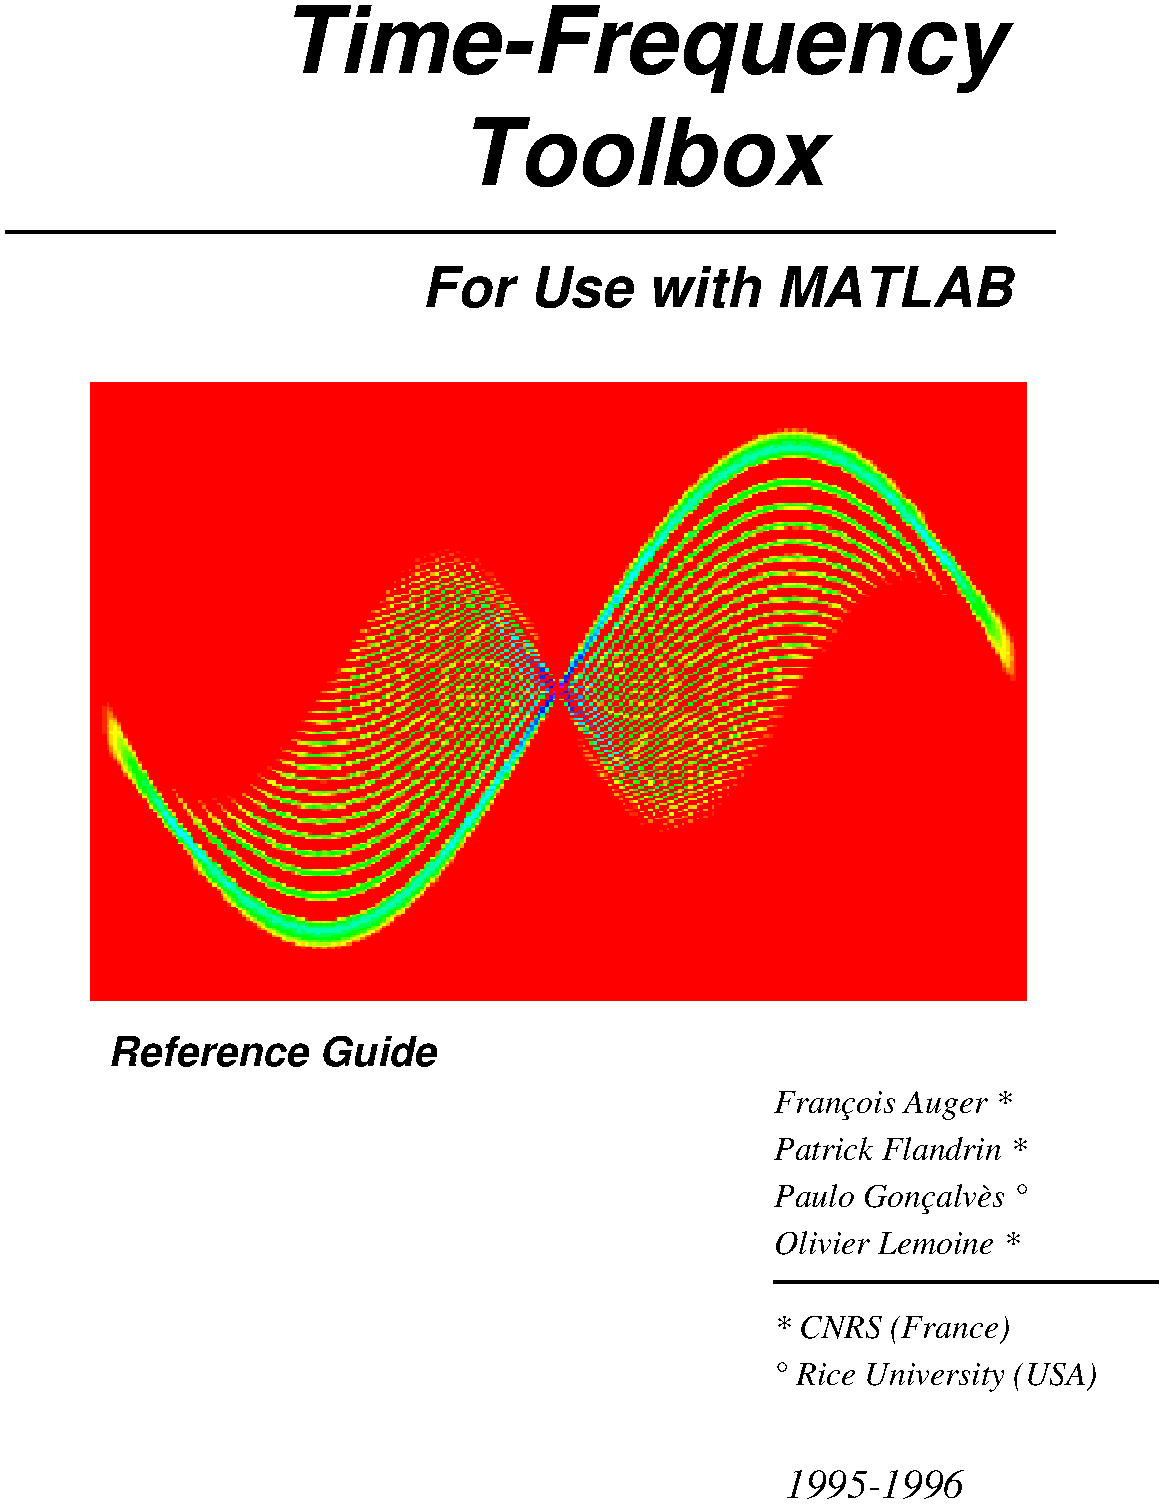
\includegraphics[width=16.8cm,height=23.8cm]{figure/coverrg}}
\end{figure}

\end{latexonly}

\cleardoublepage

\begin{htmlonly}
\section*{Forewords}
\end{htmlonly}

\centerline{
\includegraphics[width=5cm]{figure/cnrs}\hspace{2cm}
            
\includegraphics[width=5cm]{figure/isis}}

\vspace{2 cm}
Copyright (C)  1996 CNRS (France) and Rice University (USA).\\
Permission is granted to copy, distribute and/or modify this document
under the terms of the GNU Free Documentation License, Version 1.2
or any later version published by the Free Software Foundation;
with no Invariant Sections, no Front-Cover Texts, and no Back-Cover
Texts.  A copy of the license is included in the section entitled "GNU
Free Documentation License".

\vspace{2 cm}
The Time-Frequency Toolbox has been mainly developed under the auspices of
the French CNRS ({\em Centre National de la Recherche Scientifique}). It
results from a research effort conducted within its Groupements de
Recherche "Traitement du Signal et Images" (O. Macchi) and "Information,
Signal et Images" (J.-M. Chassery). Parts of the Toolbox have also been
developed at Rice University, when one of the authors (PG) was visiting the
Department of Electrical and Computer Engineering, supported by NSF.
Supporting institutions are gratefully acknowledged, as well as M.
Guglielmi, M. Najim, R. Settineri, R.G. Baraniuk, M. Chausse, D. Roche,
E. Chassande-Mottin, O. Michel and P. Abry for their help at different 
phases of the development.

\cleardoublepage

\pagestyle{myheadings}
% This is part of the TFTB Reference Manual.
% Copyright (C) 1996 CNRS (France) and Rice University (US).
% See the file refguide.tex for copying conditions.


\section*{Glossary and summary}

This section contains detailed descriptions of all the Time-Frequency Toolbox
functions. It begins with a glossary and a list of functions grouped by
subject area and continues with the reference entries in alphabetical
order. Information is also available through the online help facility.

\vspace*{1cm}

\begin{center}
\begin{tabular}{|c|c|}
\hline 
AF & Ambiguity function\\
AR & Auto-regressive (filter or model)\\
ASK & Amplitude shift keyed signal\\
BJD & Born-Jordan distribution\\
BPSK & Binary phase shift keyed signal\\
BUD & Butterworth distribution\\
CWD & Choi-Williams distribution\\
FM & Frequency modulation\\
FSK & Frequency shift keyed signal\\
GRD & Generalized rectangular distribution\\
HT & Hough transform\\
MHD & Margenau-Hill distribution \\
MHSD & Margenau-Hill-Spectrogram distribution \\ 
MMCE & Minimum mean cross-entropy\\
NAF & Narrow-band ambiguity function\\
PMHD & Pseudo Margenau-Hill distribution\\
PWVD & Pseudo Wigner-Ville distribution\\
QPSK & Quaternary phase shift keyed signal\\
RID & Reduced interference distribution\\
STFT & Short-time Fourier transform\\
TFR & Time-frequency representation\\
WAF & Wide-band ambiguity function\\
WVD & Wigner-Ville distribution\\
ZAM & Zhao-Atlas-Marks distribution\\
\hline 
\end{tabular} 
\end{center}


\addcontentsline{toc}{chapter}{Reference Guide}
\addcontentsline{toc}{section}{Tables}
\newpage % This is part of the TFTB Reference Manual.
% Copyright (C) 1996 CNRS (France) and Rice University (US).
% See the file refguide.tex for copying conditions.


\begin{itemize}
\item {\bf Signal generation files}

\hspace*{-1cm}
\begin{tabular}{|p{2.5cm} p{11cm}|}
\hline
\multicolumn{2}{|c|}{\bf Choice of the Instantaneous Amplitude }\\
\hline
 {\ty amexpo1s} &  One-sided exponential amplitude modulation\\
 {\ty amexpo2s} &  Bilateral exponential amplitude modulation\\
 {\ty amgauss } &  Gaussian amplitude modulation\\
 {\ty amrect  } &  Rectangular amplitude modulation\\
 {\ty amtriang} &  Triangular amplitude modulation\\
\hline
\end{tabular}
%\vspace*{.5cm}

\hspace*{-1cm}
\begin{tabular}{|p{2.5cm} p{11cm}|}
\hline
\multicolumn{2}{|c|}{\bf Choice of the Instantaneous Frequency }\\
\hline
 {\ty fmconst } & Signal with constant frequency modulation\\
 {\ty fmhyp   } & Signal with hyperbolic frequency modulation\\
 {\ty fmlin   } & Signal with linear frequency modulation\\
 {\ty fmodany } & Signal with arbitrary frequency modulation\\
 {\ty fmpar   } & Signal with parabolic frequency modulation\\
 {\ty fmpower } & Signal with power-law frequency modulation\\
 {\ty fmsin   } & Signal with sinusoidal frequency modulation\\
 {\ty gdpower } & Signal with a power-law group delay\\
\hline
\end{tabular}
%\vspace*{.5cm}

\hspace*{-1cm}
\begin{tabular}{|p{2.5cm} p{11cm}|}
\hline
\multicolumn{2}{|c|}{\bf Choice of Particular Signals }\\
\hline
 {\ty altes   } & Altes signal in time domain\\
 {\ty anaask  } & Amplitude Shift Keyed (ASK) signal\\
 {\ty anabpsk } & Binary Phase Shift Keyed (BPSK) signal\\
 {\ty anafsk  } & Frequency Shift Keyed (FSK) signal\\
 {\ty anapulse} & Analytic projection of unit amplitude impulse signal\\
 {\ty anaqpsk } & Quaternary Phase Shift Keyed (QPSK) signal\\
 {\ty anasing } & Lipschitz singularity\\
 {\ty anastep } & Analytic projection of unit step signal\\
 {\ty atoms   } & Linear combination of elementary Gaussian atoms\\ 
 {\ty dopnoise} & Complex Doppler random signal\\
 {\ty doppler } & Complex Doppler signal\\
 {\ty klauder } & Klauder wavelet in time domain\\
 {\ty mexhat  } & Mexican hat wavelet in time domain\\
 {\ty window  } & Window generation\\
\hline
\end{tabular}
%\vspace*{.5cm}

\hspace*{-1cm}
\begin{tabular}{|p{2.5cm} p{11cm}|}
\hline
\multicolumn{2}{|c|}{\bf Noise Realizations}\\
\hline
 {\ty noisecg } & Analytic complex gaussian noise\\
 {\ty noisecu } & Analytic complex uniform white noise\\
\hline
\end{tabular}
%\vspace*{.5cm}

\hspace*{-1cm}
\begin{tabular}{|p{2.5cm} p{11cm}|}
\hline
\multicolumn{2}{|c|}{\bf  Modification}\\
\hline
 {\ty scale   } & Scale a signal using the Mellin transform\\
 {\ty sigmerge} & Add two signals with a given energy ratio in dB\\
\hline
\end{tabular}


\item {\bf Processing files}

\hspace*{-1cm}
\begin{tabular}{|p{2.5cm} p{11cm}|}
\hline
\multicolumn{2}{|c|}{\bf  Time-Domain Processing}\\
\hline
 {\ty ifestar2} & Instantaneous frequency estimation using AR2 modelisation.\\
 {\ty instfreq} & Instantaneous frequency estimation\\
 {\ty loctime } & Time localization characteristics\\
\hline
\end{tabular}
%\vspace*{.5cm}

\hspace*{-1cm}
\begin{tabular}{|p{2.5cm} p{11cm}|}
\hline
\multicolumn{2}{|c|}{\bf  Frequency-Domain Processing}\\
\hline
 {\ty fmt     } & Fast Mellin transform\\
 {\ty ifmt    } & Inverse fast Mellin transform\\
 {\ty locfreq } & Frequency localization characteristics\\
 {\ty sgrpdlay} & Group delay estimation\\
\hline
\end{tabular}
%\vspace*{.5cm}

\hspace*{-1cm}
\begin{tabular}{|p{2.5cm} p{11cm}|}
\hline
\multicolumn{2}{|c|}{\bf Linear Time-Frequency Processing }\\
\hline
 {\ty tfrgabor} & Gabor representation\\
 {\ty tfrstft } & Short time Fourier transform\\
\hline
\end{tabular}
%\vspace*{.5cm}

\hspace*{-1cm}
\begin{tabular}{|p{2.5cm} p{11cm}|}\hline
\multicolumn{2}{|c|}{\bf Bilinear Time-Frequency Processing in the Cohen's Class }\\
\hline
 {\ty tfrbj   } & Born-Jordan distribution\\                     
 {\ty tfrbud  } & Butterworth distribution\\                   
 {\ty tfrcw   } & Choi-Williams distribution\\                   
 {\ty tfrgrd  } & Generalized rectangular distribution\\        
 {\ty tfrmh   } & Margenau-Hill distribution\\                    
 {\ty tfrmhs  } & Margenau-Hill-Spectrogram distribution\\     
 {\ty tfrmmce } & Minimum mean cross-entropy combination of spectrograms\\ 
 {\ty tfrpage } & Page distribution\\                          
 {\ty tfrpmh  } & Pseudo Margenau-Hill distribution\\          
 {\ty tfrppage} & Pseudo Page distribution\\                 
 {\ty tfrpwv  } & Pseudo Wigner-Ville distribution\\            
 {\ty tfrri   } & Rihaczek distribution\\                       
 {\ty tfrridb } & Reduced interference distribution (Bessel window)\\
 {\ty tfrridbn} & Reduced interference distribution (binomial window)\\
 {\ty tfrridh } & Reduced interference distribution (Hanning window)\\
 {\ty tfrridt } & Reduced interference distribution (triangular window)\\
 {\ty tfrsp   } & Spectrogram distribution\\                     
 {\ty tfrspwv } & Smoothed Pseudo Wigner-Ville distribution\\   
 {\ty tfrwv   } & Wigner-Ville distribution\\
 {\ty tfrzam  } & Zhao-Atlas-Marks distribution\\               
\hline
\end{tabular}
%\vspace*{.5cm}

\hspace*{-1cm}
\begin{tabular}{|p{2.5cm} p{11cm}|}
\hline
\multicolumn{2}{|c|}{\bf Bilinear Time-Frequency Processing in the Affine Class }\\
\hline
 {\ty tfrbert } & Unitary Bertrand distribution\\
 {\ty tfrdfla } & D-Flandrin distribution\\
 {\ty tfrscalo} & Scalogram, for Morlet or Mexican hat wavelet\\
 {\ty tfrspaw } & Smoothed Pseudo Affine Wigner distributions\\
 {\ty tfrunter} & Unterberger distribution, active or passive form\\
\hline
\end{tabular}
%\vspace*{.5cm}

\hspace*{-1cm}
\begin{tabular}{|p{2.5cm} p{11cm}|}
\hline
\multicolumn{2}{|c|}{\bf  Reassigned Time-Frequency Processing}\\
\hline
 {\ty tfrrgab } & Reassigned Gabor spectrogram\\
 {\ty tfrrmsc } & Reassigned Morlet Scalogram time-frequency distribution\\
 {\ty tfrrpmh } & Reassigned Pseudo Margenau-Hill distribution\\
 {\ty tfrrppag} & Reassigned Pseudo Page distribution\\
 {\ty tfrrpwv } & Reassigned Pseudo Wigner-Ville distribution\\
 {\ty tfrrsp  } & Reassigned Spectrogram\\ 
 {\ty tfrrspwv} & Reassigned Smoothed Pseudo WV distribution\\
\hline
\end{tabular}
%\vspace*{.5cm}

\hspace*{-1cm}
\begin{tabular}{|p{2.5cm} p{11cm}|}
\hline
\multicolumn{2}{|c|}{\bf Ambiguity Functions }\\
\hline
 {\ty ambifunb} & Narrow-band ambiguity function\\
 {\ty ambifuwb} & Wide-band ambiguity function\\
\hline
\end{tabular}
%\vspace*{.5cm}

\hspace*{-1cm}
\begin{tabular}{|p{2.5cm} p{11cm}|}
\hline
\multicolumn{2}{|c|}{\bf Post-Processing or Help to the Interpretation }\\
\hline
 {\ty friedman} & Instantaneous frequency density\\
 {\ty holder  } & Estimation of the H�lder exponent through an affine TFR\\
 {\ty htl     } & Hough transform for detection of lines in images\\
 {\ty margtfr } & Marginals and energy of a time-frequency representation\\
 {\ty midpoint} & Mid-point construction used in the interference diagram\\ 
 {\ty momftfr } & Frequency moments of a time-frequency representation\\
 {\ty momttfr } & Time moments of a time-frequency representation\\
 {\ty plotsid } & Schematic interference diagram of FM signals\\ 
 {\ty renyi   } & Measure Renyi information\\
 {\ty ridges  } & Extraction of ridges from a reassigned TFR\\
 {\ty tfrideal} & Ideal TFR for given frequency laws\\
\hline
\end{tabular}
%\vspace*{.5cm}

\hspace*{-1cm}
\begin{tabular}{|p{2.5cm} p{11cm}|}
\hline
\multicolumn{2}{|c|}{\bf  Visualization and backup}\\
\hline
 {\ty plotifl } & Plot normalized instantaneous frequency laws\\
 {\ty tfrparam} & Return the paramaters needed to display (or save) a TFR\\
 {\ty tfrqview} & Quick visualization of a time-frequency representation\\
 {\ty tfrsave } & Save the parameters of a time-frequency representation\\
 {\ty tfrview } & Visualization of time-frequency representations\\
\hline
\end{tabular}
%\vspace*{.5cm}

\hspace*{-1cm}
\begin{tabular}{|p{2cm} p{12cm}|}
\hline
\multicolumn{2}{|c|}{\bf Other }\\
\hline
 {\ty disprog } & Display the progression of a loop\\
 {\ty divider } & Find dividers of an integer, closest from the square root
		  of the integer \\ 
 {\ty dwindow } & Derive a window\\
 {\ty integ   } & Approximate an integral\\
 {\ty integ2d } & Approximate a 2-D integral\\
 {\ty izak    } & Inverse Zak transform\\
 {\ty kaytth  } & Computation of the Kay-Tretter filter\\
 {\ty modulo  } & Congruence of a vector\\
 {\ty movcw4at} & Four atoms rotating, analyzed by the Choi-Williams distribution\\
 {\ty movpwdph} & Influence of a phase-shift on the interferences of the PWVD\\
 {\ty movpwjph} & Influence of a jump of phase on the interferences of the PWVD\\
 {\ty movsc2wv} & Movie illustrating the passage from the scalogram to the WVD\\
 {\ty movsp2wv} & Movie illustrating the passage from the spectrogram to the WVD\\
 {\ty movwv2at} & Oscillating structure of the interferences of the WVD\\  
 {\ty odd     } & Round towards nearest odd value\\
 {\ty zak     } & Zak transform\\
\hline
\end{tabular}
\end{itemize}


\tableofcontents
\newpage \indexsection{altes} % This is part of the TFTB Reference Manual.
% Copyright (C) 1996 CNRS (France) and Rice University (US).
% See the file refguide.tex for copying conditions.


\markright{altes}
\section*{\hspace*{-1.6cm} altes}

\vspace*{-.4cm}
\hspace*{-1.6cm}\rule[0in]{16.5cm}{.02cm}
\vspace*{.2cm}



{\bf \large \sf Purpose}\\
\hspace*{1.5cm}
\begin{minipage}[t]{13.5cm}
Altes signal in time domain.
\end{minipage}
\vspace*{.5cm}


{\bf \large \sf Synopsis}\\
\hspace*{1.5cm}
\begin{minipage}[t]{13.5cm}
\begin{verbatim}
x = altes(N)
x = altes(N,fmin)
x = altes(N,fmin,fmax)
x = altes(N,fmin,fmax,alpha)
\end{verbatim}
\end{minipage}
\vspace*{.5cm}


{\bf \large \sf Description}\\
\hspace*{1.5cm}
\begin{minipage}[t]{13.5cm}
        {\ty altes} generates the Altes signal in
        the time domain.\\
 
\hspace*{-.5cm}
\begin{tabular*}{14cm}{p{1.5cm} p{8.5cm} c}
Name & Description & Default value\\
\hline
	{\ty N}&number of points in time&  \\ 
	{\ty fmin}&lower frequency bound (value of the hyperbolic
                instantaneous frequency law at the sample {\ty N}), 
                in normalized frequency&{\ty 0.05}\\
	{\ty fmax}&upper frequency bound (value of the hyperbolic
                instantaneous frequency law at the first sample), 
                in normalized frequency            &{\ty 0.5}\\
        {\ty alpha}&attenuation factor of the envelope & {\ty 300}\\
  \hline {\ty x}&time row vector containing the Altes signal samples\\
\hline
\end{tabular*}

\end{minipage}
\vspace*{1cm}


{\bf \large \sf Example}\\
\hspace*{1.5cm}
\begin{minipage}[t]{13.5cm}
\begin{verbatim}
         x=altes(128,0.1,0.45); plot(x);
\end{verbatim}
plots an Altes signal of 128 points whose normalized frequency goes from
0.45 down to 0.1.
\end{minipage}
\vspace*{.5cm}


{\bf \large \sf See Also}\\
\hspace*{1.5cm}
\begin{minipage}[t]{13.5cm}
\begin{verbatim}
klauder, anasing, anapulse, anastep, doppler.
\end{verbatim}
\end{minipage}


\newpage \indexsection{ambifunb} % This is part of the TFTB Reference Manual.
% Copyright (C) 1996 CNRS (France) and Rice University (US).
% See the file refguide.tex for copying conditions.


\markright{ambifunb}
\section*{\hspace*{-1.6cm} ambifunb}

\vspace*{-.4cm}
\hspace*{-1.6cm}\rule[0in]{16.5cm}{.02cm}
\vspace*{.2cm}


{\bf \large \sf Purpose}\\
\hspace*{1.5cm}
\begin{minipage}[t]{13.5cm}
Narrow-band ambiguity function.
\end{minipage}
\vspace*{.5cm}


{\bf \large \sf Synopsis}\\
\hspace*{1.5cm}
\begin{minipage}[t]{13.5cm}
\begin{verbatim}
[naf,tau,xi] = ambifunb(x)
[naf,tau,xi] = ambifunb(x,tau)
[naf,tau,xi] = ambifunb(x,tau,N)
[naf,tau,xi] = ambifunb(x,tau,N,trace)
\end{verbatim}
\end{minipage}
\vspace*{.5cm}


{\bf \large \sf Description}\\
\hspace*{1.5cm}
\begin{minipage}[t]{13.5cm}
        {\ty ambifunb} computes the narrow-band ambiguity function of a
        signal, or the cross-ambiguity function between two signals. Its
        definition is given by
\[A_x(\xi,\tau)=\int_{-\infty}^{+\infty} x(s+\tau/2)\ x^*(s-\tau/2)\
e^{-j2\pi \xi s}\ ds.\] 

\hspace*{-.5cm}
\begin{tabular*}{14cm}{p{1.5cm} p{8.5cm} c}
Name & Description & Default value\\ 
\hline 
{\ty x} & signal if auto-AF, or {\ty [x1,x2]} if cross-AF ({\ty length(x)=Nx})&\\ 
{\ty tau} & vector of lag values &{\ty (-Nx/2:Nx/2)}\\ 
{\ty N} & number of frequency bins &{\ty Nx}\\ 
{\ty trace} & if non-zero, the progression of the algorithm is shown&{\ty 0}\\ 
\hline
{\ty naf} & doppler-lag representation, with the doppler bins stored in the rows
and the time-lags stored in the columns&\\ 
{\ty xi} & vector of doppler values\\\hline
\end{tabular*}
\vspace*{.5cm}

This representation is computed such as its 2D Fourier transform equals the
Wigner-Ville distribution.  When called without output arguments, {\ty
ambifunb} displays the squared modulus of the ambiguity function by means
of {\ty contour}.

The ambiguity function is a measure of the time-frequency correlation of a
signal $x$, i.e. the degree of similarity between $x$ and its translated
versions in the time-frequency plane.
\end{minipage}
\vspace*{1cm}

\newpage

{\bf \large \sf Examples}\\
\hspace*{1.5cm}
\begin{minipage}[t]{13.5cm}
Consider a BPSK signal (see {\ty anabpsk}) of 256 points, with a keying
period of 8 points, and analyze it with the narrow-band ambiguity
function\,:
\begin{verbatim}
         sig=anabpsk(256,8);
         ambifunb(sig);
\end{verbatim}
The resulting function presents a high thin peak at the origin of the
ambiguity plane, with small sidelobes around. This means that the
inter-correlation between this signal and a time/frequency-shifted version
of it is nearly zero (the ambiguity in the estimation of its arrival time
and mean-frequency is very small).\\

Here is an other example that checks the correspondance between the WVD and
the narrow-band ambiguity function by means of a 2D Fourier transform\,:
\begin{verbatim}
         N=128; sig=fmlin(N); amb=ambifunb(sig);
         amb=amb([N/2+1:N 1:N/2],:);
         ambi=ifft(amb).';
         tdr=zeros(N); 		% Time-delay representation
         tdr(1:N/2,:)=ambi(N/2:N-1,:);
         tdr(N:-1:N/2+2,:)=ambi(N/2-1:-1:1,:);
         wvd1=real(fft(tdr));

         wvd2=tfrwv(sig);
         diff=max(max(abs(wvd1-wvd2)))
         diff = 
                1.5632e-13
\end{verbatim}
\end{minipage}
\vspace*{.5cm}


{\bf \large \sf See Also}\\
\hspace*{1.5cm}
\begin{minipage}[t]{13.5cm}
\begin{verbatim}
ambifuwb.
\end{verbatim}
\end{minipage}

 
\newpage \indexsection{ambifuwb} % This is part of the TFTB Reference Manual.
% Copyright (C) 1996 CNRS (France) and Rice University (US).
% See the file refguide.tex for copying conditions.


\markright{ambifuwb}
\section*{\hspace*{-1.6cm} ambifuwb}

\vspace*{-.4cm}
\hspace*{-1.6cm}\rule[0in]{16.5cm}{.02cm}
\vspace*{.2cm}



{\bf \large \sf Purpose}\\
\hspace*{1.5cm}
\begin{minipage}[t]{13.5cm}
Wide-band ambiguity function.
\end{minipage}
\vspace*{.5cm}


{\bf \large \sf Synopsis}\\
\hspace*{1.5cm}
\begin{minipage}[t]{13.5cm}
\begin{verbatim}
[waf,tau,theta] = ambifuwb(x)
[waf,tau,theta] = ambifuwb(x,fmin,fmax)
[waf,tau,theta] = ambifuwb(x,fmin,fmax,N)
[waf,tau,theta] = ambifuwb(x,fmin,fmax,N,trace)
\end{verbatim}
\end{minipage}
\vspace*{.5cm}


{\bf \large \sf Description}\\
\hspace*{1.5cm}
\begin{minipage}[t]{13.5cm}
        {\ty ambifuwb} calculates the asymetric wide-band ambiguity
        function, defined as 
\begin{eqnarray*}
\Xi_x(a,\tau) = \frac{1}{\sqrt{a}}\ \int_{-\infty}^{+\infty} x(t)\
x^*(t/a-\tau)\ dt = \sqrt{a} \int_{-\infty}^{+\infty} X(\nu)\ X^*(a\nu)\
e^{j2\pi a \tau\nu}\ d\nu. 
\end{eqnarray*}

\hspace*{-.5cm}\begin{tabular*}{14cm}{p{1.5cm} p{8.5cm} c}
Name & Description & Default value\\
\hline
        {\ty x}     & signal (in time) to be analyzed (the analytic associated
                signal is considered), of length {\ty Nx} &\\
        {\ty fmin, fmax} & respectively lower and upper frequency bounds of
                the analyzed signal. When specified, these parameters fix
                the equivalent frequency bandwidth (both are expressed in
                Hz)             & {\ty 0, 0.5}\\
        {\ty N}     & number of Mellin points. This number is needed when {\ty fmin}
                and {\ty fmax} are forced     & {\ty Nx}\\
        {\ty trace} & if non-zero, the progression of the algorithm is shown
                                        & 0\\
\hline
        {\ty waf}    & matrix containing the coefficients of the ambiguity
                function. X-coordinate corresponds to the dual variable of 
                scale parameter ; Y-coordinate corresponds to time delay,
                dual variable of frequency.\\
        {\ty tau}   & X-coordinate corresponding to time delay\\
        {\ty theta} & Y-coordinate corresponding to the $\log(a)$ variable,
		where $a$ is the scale\\
\hline
\end{tabular*}
\vspace*{.2cm}

When called without output arguments, {\ty ambifuwb} displays the squared
modulus of the ambiguity function by means of {\ty contour}.
\end{minipage}

\newpage

{\bf \large \sf Example}\\
\hspace*{1.5cm}
\begin{minipage}[t]{13.5cm}
Consider a BPSK signal (see {\ty anabpsk}) of 256 points, with a keying
period of 8 points, and analyze it with the wide-band ambiguity
function\,:
\begin{verbatim}
         sig=anabpsk(256,8);
         ambifunb(sig);
\end{verbatim}
The result, to be compared with the one obtained with the narrow-band
ambiguity function, presents a thin high peak at the origin of the
ambiguity plane, but with more important sidelobes than with the
narrow-band ambiguity function. It means that the narrow-band assumption is
not very well adapted to this signal, and that the ambiguity in the
estimation of its arrival time and mean frequency is not so small.
\end{minipage}
\vspace*{.5cm}


{\bf \large \sf See Also}\\
\hspace*{1.5cm}
\begin{minipage}[t]{13.5cm}
\begin{verbatim}
ambifunb.
\end{verbatim}
\end{minipage}

 
\newpage \indexsection{amexpo1s} % This is part of the TFTB Reference Manual.
% Copyright (C) 1996 CNRS (France) and Rice University (US).
% See the file refguide.tex for copying conditions.


\markright{amexpo1s}
\section*{\hspace*{-1.6cm} amexpo1s}

\vspace*{-.4cm}
\hspace*{-1.6cm}\rule[0in]{16.5cm}{.02cm}
\vspace*{.2cm}



{\bf \large \sf Purpose}\\
\hspace*{1.5cm}
\begin{minipage}[t]{13.5cm}
One-sided exponential amplitude modulation.
\end{minipage}
\vspace*{.5cm}


{\bf \large \sf Synopsis}\\
\hspace*{1.5cm}
\begin{minipage}[t]{13.5cm}
\begin{verbatim}
y = amexpo1s(N)
y = amexpo1s(N,t0)
y = amexpo1s(N,t0,T)
\end{verbatim}
\end{minipage}
\vspace*{.5cm}


{\bf \large \sf Description}\\
\hspace*{1.5cm}
\begin{minipage}[t]{13.5cm}
        {\ty amexpo1s} generates a one-sided exponential amplitude
        modulation starting at time {\ty t0}, and with a spread proportional to
        {\ty T}.\\ This modulation is scaled such that {\ty y(t0)=1}.\\
  
\hspace*{-.5cm}\begin{tabular*}{14cm}{p{1.5cm} p{8.5cm} c}
Name & Description & Default value\\
\hline
        {\ty N}  & number of points\\
        {\ty t0} & arrival time of the exponential   & {\ty N/2}\\
        {\ty T}  & time spreading                    & {\ty 2*sqrt(N)}\\
  \hline {\ty y}  & signal\\
\hline
\end{tabular*}
\end{minipage}
\vspace*{1cm}


{\bf \large \sf Examples}
\begin{verbatim}
         z=amexpo1s(160);       plot(z);
         z=amexpo1s(160,20,40); plot(z);
\end{verbatim}
\vspace*{.5cm}


{\bf \large \sf See Also}\\
\hspace*{1.5cm}
\begin{minipage}[t]{13.5cm}
\begin{verbatim}
amexpo2s, amgauss, amrect, amtriang.
\end{verbatim}
\end{minipage}


 
\newpage \indexsection{amexpo2s} % This is part of the TFTB Reference Manual.
% Copyright (C) 1996 CNRS (France) and Rice University (US).
% See the file refguide.tex for copying conditions.


\markright{amexpo2s}
\section*{\hspace*{-1.6cm} amexpo2s}

\vspace*{-.4cm}
\hspace*{-1.6cm}\rule[0in]{16.5cm}{.02cm}
\vspace*{.2cm}



{\bf \large \sf Purpose}\\
\hspace*{1.5cm}
\begin{minipage}[t]{13.5cm}
Bilateral exponential amplitude modulation.
\end{minipage}
\vspace*{.5cm}


{\bf \large \sf Synopsis}\\
\hspace*{1.5cm}
\begin{minipage}[t]{13.5cm}
\begin{verbatim}
y = amexpo2s(N)
y = amexpo2s(N,t0)
y = amexpo2s(N,t0,T)
\end{verbatim}
\end{minipage}
\vspace*{.5cm}


{\bf \large \sf Description}\\
\hspace*{1.5cm}
\begin{minipage}[t]{13.5cm}
        {\ty amexpo2s} generates a bilateral exponential amplitude
        modulation centered on a time {\ty t0}, and with a spread
        proportional to {\ty T}.\\ This modulation is scaled such that {\ty
        y(t0)=1}.\\

\hspace*{-.5cm}\begin{tabular*}{14cm}{p{1.5cm} p{8.5cm} c}
Name & Description & Default value\\
\hline
        {\ty N } & number of points\\
        {\ty t0} & time center       &          {\ty N/2}\\
        {\ty T}  & time spreading     &        {\ty 2*sqrt(N)}\\
  \hline {\ty y}  & signal\\

\hline
\end{tabular*}

\end{minipage}
\vspace*{1cm}


{\bf \large \sf Examples}
\begin{verbatim}
         z=amexpo2s(160);        plot(z);
         z=amexpo2s(160,90,40);  plot(z);
         z=amexpo2s(160,180,50); plot(z);
\end{verbatim}
\vspace*{.5cm}


{\bf \large \sf See Also}\\
\hspace*{1.5cm}
\begin{minipage}[t]{13.5cm}
\begin{verbatim}
amexpo1s, amgauss, amrect, amtriang.
\end{verbatim}
\end{minipage}

 
\newpage \indexsection{amgauss} % This is part of the TFTB Reference Manual.
% Copyright (C) 1996 CNRS (France) and Rice University (US).
% See the file refguide.tex for copying conditions.


\markright{amgauss}
\section*{\hspace*{-1.6cm} amgauss}

\vspace*{-.4cm}
\hspace*{-1.6cm}\rule[0in]{16.5cm}{.02cm}
\vspace*{.2cm}



{\bf \large \sf Purpose}\\
\hspace*{1.5cm}
\begin{minipage}[t]{13.5cm}
Gaussian amplitude modulation.
\end{minipage}
\vspace*{.5cm}


{\bf \large \sf Synopsis}\\
\hspace*{1.5cm}
\begin{minipage}[t]{13.5cm}
\begin{verbatim}
y = amgauss(N)
y = amgauss(N,t0)
y = amgauss(N,t0,T)
\end{verbatim}
\end{minipage}
\vspace*{.5cm}


{\bf \large \sf Description}\\
\hspace*{1.5cm}
\begin{minipage}[t]{13.5cm}
        {\ty amgauss} generates a gaussian amplitude modulation centered on
        a time {\ty t0}, and with a spread proportional to {\ty T}.  This
        modulation is scaled such that {\ty y(t0)=1} and {\ty y(t0+T/2)}
        and {\ty y(t0-T/2)} are approximately equal to 0.5~:
        $$y(t)=e^{-\pi\left({t-t_0\over T}\right)^2}$$

\hspace*{-.5cm}\begin{tabular*}{14cm}{p{1.5cm} p{8.5cm} c}
Name & Description & Default value\\
\hline
        {\ty N}  & number of points\\
        {\ty t0} & time center       &         {\ty N/2}\\
        {\ty T}  & time spreading    &         {\ty 2*sqrt(N)}\\
  \hline {\ty y}  & signal\\
\hline
\end{tabular*}
\end{minipage}
\vspace*{1cm}


{\bf \large \sf Examples}
\begin{verbatim}
         z=amgauss(160);        plot(z);
         z=amgauss(160,90,40);  plot(z);
         z=amgauss(160,180,50); plot(z);
\end{verbatim}
\vspace*{.5cm}


{\bf \large \sf See Also}\\
\hspace*{1.5cm}
\begin{minipage}[t]{13.5cm}
\begin{verbatim}
amexpo1s, amexpo2s, amrect, amtriang.
\end{verbatim}
\end{minipage}

 
\newpage \indexsection{amrect} % This is part of the TFTB Reference Manual.
% Copyright (C) 1996 CNRS (France) and Rice University (US).
% See the file refguide.tex for copying conditions.



\markright{amrect}
\section*{\hspace*{-1.6cm} amrect}

\vspace*{-.4cm}
\hspace*{-1.6cm}\rule[0in]{16.5cm}{.02cm}
\vspace*{.2cm}



{\bf \large \sf Purpose}\\
\hspace*{1.5cm}
\begin{minipage}[t]{13.5cm}
Rectangular amplitude modulation.
\end{minipage}
\vspace*{.5cm}


{\bf \large \sf Synopsis}\\
\hspace*{1.5cm}
\begin{minipage}[t]{13.5cm}
\begin{verbatim}
y = amrect(N)
y = amrect(N,t0)
y = amrect(N,t0,T)
\end{verbatim}
\end{minipage}
\vspace*{.5cm}


{\bf \large \sf Description}\\
\hspace*{1.5cm}
\begin{minipage}[t]{13.5cm}
        {\ty amrect} generates a rectangular amplitude modulation centered
        on a time {\ty t0}, and with a spread proportional to {\ty T}.
        This modulation is scaled such that {\ty y(t0)=1}.\\

\hspace*{-.5cm}\begin{tabular*}{14cm}{p{1.5cm} p{8.5cm} c}
Name & Description & Default value\\
\hline
        {\ty N}  & number of points\\
        {\ty t0} & time center       &         {\ty N/2}\\
        {\ty T}  & time spreading    &         {\ty 2*sqrt(N)}\\
  \hline {\ty y}  & signal\\
\hline
\end{tabular*}

\end{minipage}
\vspace*{1cm}


{\bf \large \sf Examples}
\begin{verbatim}
         z=amrect(160);        plot(z);
         z=amrect(160,90,40);  plot(z);
         z=amrect(160,180,70); plot(z);
\end{verbatim}
\vspace*{.5cm}


{\bf \large \sf See Also}\\
\hspace*{1.5cm}
\begin{minipage}[t]{13.5cm}
\begin{verbatim}
amexpo1s, amexpo2s, amgauss, amtriang.
\end{verbatim}
\end{minipage}



 
\newpage \indexsection{amtriang} % This is part of the TFTB Reference Manual.
% Copyright (C) 1996 CNRS (France) and Rice University (US).
% See the file refguide.tex for copying conditions.


\markright{amtriang}
\section*{\hspace*{-1.6cm} amtriang}

\vspace*{-.4cm}
\hspace*{-1.6cm}\rule[0in]{16.5cm}{.02cm}
\vspace*{.2cm}



{\bf \large \sf Purpose}\\
\hspace*{1.5cm}
\begin{minipage}[t]{13.5cm}
Triangular amplitude modulation.
\end{minipage}
\vspace*{.5cm}


{\bf \large \sf Synopsis}\\
\hspace*{1.5cm}
\begin{minipage}[t]{13.5cm}
\begin{verbatim}
y = amtriang(N)
y = amtriang(N,t0)
y = amtriang(N,t0,T)
\end{verbatim}
\end{minipage}
\vspace*{.5cm}


{\bf \large \sf Description}\\
\hspace*{1.5cm}
\begin{minipage}[t]{13.5cm}
        {\ty amtriang} generates a triangular amplitude modulation 
        centered on a time {\ty t0}, and with a spread proportional to {\ty T}.
        This modulation is scaled such that {\ty y(t0)=1}.\\

\hspace*{-.5cm}\begin{tabular*}{14cm}{p{1.5cm} p{8.5cm} c}
Name & Description & Default value\\
\hline
        {\ty N}  & number of points\\
        {\ty t0} & time center       &          {\ty N/2}\\
        {\ty T}  & time spreading    &          {\ty 2*sqrt(N)}\\
  \hline {\ty y}  & signal\\
\hline
\end{tabular*}

\end{minipage}
\vspace*{1cm}


{\bf \large \sf Examples}
\begin{verbatim}
         z=amtriang(160);        plot(z);
         z=amtriang(160,90,40);  plot(z);
         z=amtriang(160,180,50); plot(z);
\end{verbatim}
\vspace*{.5cm}


{\bf \large \sf See Also}\\
\hspace*{1.5cm}
\begin{minipage}[t]{13.5cm}
\begin{verbatim}
amexpo1s, amexpo2s, amgauss, amrect.
\end{verbatim}
\end{minipage}



 
\newpage \indexsection{anaask} % This is part of the TFTB Reference Manual.
% Copyright (C) 1996 CNRS (France) and Rice University (US).
% See the file refguide.tex for copying conditions.



\markright{anaask}
\section*{\hspace*{-1.6cm} anaask}

\vspace*{-.4cm}
\hspace*{-1.6cm}\rule[0in]{16.5cm}{.02cm}
\vspace*{.2cm}



{\bf \large \sf Purpose}\\
\hspace*{1.5cm}
\begin{minipage}[t]{13.5cm}
Amplitude Shift Keyed (ASK) signal.
\end{minipage}
\vspace*{.5cm}


{\bf \large \sf Synopsis}\\
\hspace*{1.5cm}
\begin{minipage}[t]{13.5cm}
\begin{verbatim}
[y,am] = anaask(N)
[y,am] = anaask(N,ncomp)
[y,am] = anaask(N,ncomp,f0)
\end{verbatim}
\end{minipage}
\vspace*{.5cm}


{\bf \large \sf Description}\\
\hspace*{1.5cm}
\begin{minipage}[t]{13.5cm}
        {\ty anaask} returns a complex amplitude modulated signal of
        normalized frequency {\ty f0}, with a uniformly distributed random
        amplitude.  Such signal is only 'quasi'-analytic.\\

\hspace*{-.5cm}\begin{tabular*}{14cm}{p{1.5cm} p{8.5cm} c}
Name & Description & Default value\\
\hline
        {\ty N }    & number of points\\
        {\ty ncomp} & number of points of each component & {\ty N/5}\\
        {\ty f0}    & normalized frequency               & {\ty 0.25}\\
  \hline {\ty y}     & signal\\
        {\ty am }   & resulting amplitude modulation     \\
\hline
\end{tabular*}

\end{minipage}
\vspace*{1cm}


{\bf \large \sf Example}
\begin{verbatim}
         [signal,am]=anaask(512,64,0.05); 
         subplot(211); plot(real(signal)); 
         subplot(212); plot(am);
\end{verbatim}
\vspace*{.5cm}


{\bf \large \sf See Also}\\
\hspace*{1.5cm}
\begin{minipage}[t]{13.5cm}
\begin{verbatim}
anafsk, anabpsk, anaqpsk.
\end{verbatim}
\end{minipage}
\vspace*{.5cm}


{\bf \large \sf Reference}\\
\hspace*{1.5cm}
\begin{minipage}[t]{13.5cm}
[1] W. Gardner {\it Statistical Spectral Analysis - A Nonprobabilistic
Theory} Englewood Cliffs, N.J. Prentice Hall, 1987.
\end{minipage}
 
\newpage \indexsection{anabpsk} % This is part of the TFTB Reference Manual.
% Copyright (C) 1996 CNRS (France) and Rice University (US).
% See the file refguide.tex for copying conditions.



\markright{anabpsk}
\section*{\hspace*{-1.6cm} anabpsk}

\vspace*{-.4cm}
\hspace*{-1.6cm}\rule[0in]{16.5cm}{.02cm}
\vspace*{.2cm}



{\bf \large \sf Purpose}\\
\hspace*{1.5cm}
\begin{minipage}[t]{13.5cm}
Binary Phase Shift Keyed (BPSK) signal.
\end{minipage}
\vspace*{.5cm}


{\bf \large \sf Synopsis}\\
\hspace*{1.5cm}
\begin{minipage}[t]{13.5cm}
\begin{verbatim}
[y,am] = anabpsk(N)
[y,am] = anabpsk(N,ncomp)
[y,am] = anabpsk(N,ncomp,f0)
\end{verbatim}
\end{minipage}
\vspace*{.5cm}


{\bf \large \sf Description}\\
\hspace*{1.5cm}
\begin{minipage}[t]{13.5cm}
        {\ty anabpsk} returns a succession of complex sinusoids of {\ty
        ncomp} points each, with a normalized frequency {\ty f0} and an
        amplitude equal to -1 or +1, according to a discrete uniform
        law. Such signal is only 'quasi'-analytic.\\

\hspace*{-.5cm}\begin{tabular*}{14cm}{p{1.5cm} p{8.5cm} c}
Name & Description & Default value\\
\hline
        {\ty N }    & number of points\\
        {\ty ncomp} & number of points of each component & {\ty N/5}\\
        {\ty f0}    & normalized frequency              & {\ty 0.25}\\
  \hline {\ty y}     & signal\\
        {\ty am}    & resulting amplitude modulation     \\
\hline
\end{tabular*}

\end{minipage}
\vspace*{1cm}


{\bf \large \sf Example}
\begin{verbatim}
         [signal,am]=anabpsk(300,30,0.1); 
         subplot(211); plot(real(signal));
         subplot(212); plot(am);
\end{verbatim}
\vspace*{.5cm}


{\bf \large \sf See Also}\\
\hspace*{1.5cm}
\begin{minipage}[t]{13.5cm}
\begin{verbatim}
anafsk, anaqpsk, anaask.
\end{verbatim}
\end{minipage}
\vspace*{.5cm}


{\bf \large \sf Reference}\\
\hspace*{1.5cm}
\begin{minipage}[t]{13.5cm}
[1] W. Gardner {\it Introduction to Random Processes, with Applications to
Signals and Systems}, 2nd Edition, McGraw-Hill, New-York, p. 360 ,1990.  
\end{minipage}
 
\newpage \indexsection{anafsk}% This is part of the TFTB Reference Manual.
% Copyright (C) 1996 CNRS (France) and Rice University (US).
% See the file refguide.tex for copying conditions.



\markright{anafsk}
\section*{\hspace*{-1.6cm} anafsk}

\vspace*{-.4cm}
\hspace*{-1.6cm}\rule[0in]{16.5cm}{.02cm}
\vspace*{.2cm}



{\bf \large \sf Purpose}\\
\hspace*{1.5cm}
\begin{minipage}[t]{13.5cm}
Frequency Shift Keyed (FSK) signal.
\end{minipage}
\vspace*{.5cm}


{\bf \large \sf Synopsis}\\
\hspace*{1.5cm}
\begin{minipage}[t]{13.5cm}
\begin{verbatim}
[y,iflaw] = anafsk(N)
[y,iflaw] = anafsk(N,ncomp)
[y,iflaw] = anafsk(N,ncomp,nbf)
\end{verbatim}
\end{minipage}
\vspace*{.5cm}


{\bf \large \sf Description}\\
\hspace*{1.5cm}
\begin{minipage}[t]{13.5cm}
        {\ty anafsk} simulates a phase coherent Frequency Shift Keyed (FSK)
        signal. This signal is a succession of complex sinusoids of {\ty ncomp}
        points each and with a normalized frequency uniformly chosen
        between {\ty nbf} distinct values between 0.0 and 0.5.  Such signal is
        only 'quasi'-analytic.\\

\hspace*{-.5cm}\begin{tabular*}{14cm}{p{1.5cm} p{8.5cm} c}
Name & Description & Default value\\
\hline
        {\ty N }    & number of points\\
        {\ty ncomp} & number of points of each component & {\ty N/5}\\
        {\ty nbf}   & number of distinct frequencies     & {\ty 4}  \\
 \hline {\ty y }    & signal\\
        {\ty iflaw} & instantaneous frequency law  \\
\hline
\end{tabular*}

\end{minipage}
\vspace*{1cm}


{\bf \large \sf Example}
\begin{verbatim}
         [signal,ifl]=anafsk(512,64,5); 
         subplot(211); plot(real(signal)); 
         subplot(212); plot(ifl);
\end{verbatim}
\vspace*{.5cm}


{\bf \large \sf See Also}\\
\hspace*{1.5cm}
\begin{minipage}[t]{13.5cm}
\begin{verbatim}
anabpsk, anaqpsk, anaask.
\end{verbatim}
\end{minipage}
\vspace*{.5cm}


{\bf \large \sf Reference}\\
\hspace*{1.5cm}
\begin{minipage}[t]{13.5cm}
[1] W. Gardner {\it Introduction to Random Processes, with Applications to
Signals and Systems}, 2nd Edition, McGraw-Hill, New-York, p. 357 ,1990.  
\end{minipage}
 
\newpage \indexsection{anapulse}% This is part of the TFTB Reference Manual.
% Copyright (C) 1996 CNRS (France) and Rice University (US).
% See the file refguide.tex for copying conditions.



\markright{anapulse}
\section*{\hspace*{-1.6cm} anapulse}

\vspace*{-.4cm}
\hspace*{-1.6cm}\rule[0in]{16.5cm}{.02cm}
\vspace*{.2cm}



{\bf \large \sf Purpose}\\
\hspace*{1.5cm}
\begin{minipage}[t]{13.5cm}
Analytic projection of unit amplitude impulse signal.
\end{minipage}
\vspace*{.5cm}


{\bf \large \sf Synopsis}\\
\hspace*{1.5cm}
\begin{minipage}[t]{13.5cm}
\begin{verbatim}
y = anapulse(N)
y = anapulse(N,ti)
\end{verbatim}
\end{minipage}
\vspace*{.5cm}


{\bf \large \sf Description}\\
\hspace*{1.5cm}
\begin{minipage}[t]{13.5cm}
        {\ty anapulse} returns an analytic N-dimensional signal 
        whose real part is a Dirac impulse at {\ty t=ti}.\\

\hspace*{-.5cm}\begin{tabular*}{14cm}{p{1.5cm} p{8.5cm} c}
Name & Description & Default value\\
\hline
        {\ty N}  & number of points\\
        {\ty ti} & time position of the impulse   & {\ty round(N/2)}\\
  \hline {\ty y}  & output signal\\
\hline
\end{tabular*}

\end{minipage}
\vspace*{1cm}


{\bf \large \sf Example}
\begin{verbatim}
         signal=2.5*anapulse(512,301);
         plot(real(signal));
\end{verbatim}
\vspace*{.5cm}


{\bf \large \sf See Also}\\
\hspace*{1.5cm}
\begin{minipage}[t]{13.5cm}
\begin{verbatim}
anastep, anasing, anabpsk, anafsk.
\end{verbatim}
\end{minipage}



 
\newpage \indexsection{anaqpsk}% This is part of the TFTB Reference Manual.
% Copyright (C) 1996 CNRS (France) and Rice University (US).
% See the file refguide.tex for copying conditions.



\markright{anaqpsk}
\section*{\hspace*{-1.6cm} anaqpsk}

\vspace*{-.4cm}
\hspace*{-1.6cm}\rule[0in]{16.5cm}{.02cm}
\vspace*{.2cm}



{\bf \large \sf Purpose}\\
\hspace*{1.5cm}
\begin{minipage}[t]{13.5cm}
Quaternary Phase Shift Keyed (QPSK) signal.
\end{minipage}
\vspace*{.5cm}


{\bf \large \sf Synopsis}\\
\hspace*{1.5cm}
\begin{minipage}[t]{13.5cm}
\begin{verbatim}
[y,pm0] = anaqpsk(N)
[y,pm0] = anaqpsk(N,ncomp)
[y,pm0] = anaqpsk(N,ncomp,f0)
\end{verbatim}
\end{minipage}
\vspace*{.5cm}


{\bf \large \sf Description}\\
\hspace*{1.5cm}
\begin{minipage}[t]{13.5cm}
        {\ty anaqpsk} returns a complex phase modulated signal of
        normalized frequency {\ty f0}, whose phase changes every {\ty
        ncomp} point according to a discrete uniform law, between the
        values {\ty (0, pi/2, pi, 3*pi/2)}.  Such signal is only
        'quasi'-analytic.\\

\hspace*{-.5cm}\begin{tabular*}{14cm}{p{1.5cm} p{8.5cm} c}
Name & Description & Default value\\
\hline
        {\ty N}     & number of points\\
        {\ty ncomp} & number of points of each component & {\ty N/5}\\
        {\ty f0}    & normalized frequency               & {\ty 0.25}\\
  \hline {\ty y}     & signal\\
        {\ty pm0}   & initial phase of each component    \\
\hline
\end{tabular*}

\end{minipage}
\vspace*{1cm}


{\bf \large \sf Example}
\begin{verbatim}
         [signal,pm0]=anaqpsk(512,64,0.05); 
         subplot(211); plot(real(signal)); 
         subplot(212); plot(pm0);
\end{verbatim}
\vspace*{.5cm}


{\bf \large \sf See Also}\\
\hspace*{1.5cm}
\begin{minipage}[t]{13.5cm}
\begin{verbatim}
anafsk, anabpsk, anaask.
\end{verbatim}
\end{minipage}
 \vspace*{.5cm}


{\bf \large \sf Reference}\\
\hspace*{1.5cm}
\begin{minipage}[t]{13.5cm}
[1] W. Gardner {\it Introduction to Random Processes, with Applications to
Signals and Systems}, 2nd Edition, McGraw-Hill, New-York, p. 362 ,1990.  
\end{minipage}


\newpage \indexsection{anasing}% This is part of the TFTB Reference Manual.
% Copyright (C) 1996 CNRS (France) and Rice University (US).
% See the file refguide.tex for copying conditions.



\markright{anasing}
\section*{\hspace*{-1.6cm} anasing}

\vspace*{-.4cm}
\hspace*{-1.6cm}\rule[0in]{16.5cm}{.02cm}
\vspace*{.2cm}



{\bf \large \sf Purpose}\\
\hspace*{1.5cm}
\begin{minipage}[t]{13.5cm}
Lipschitz singularity.
\end{minipage}
\vspace*{.5cm}


{\bf \large \sf Synopsis}\\
\hspace*{1.5cm}
\begin{minipage}[t]{13.5cm}
\begin{verbatim}
x = anasing(N)
x = anasing(N,t0)
x = anasing(N,t0,H)
\end{verbatim}
\end{minipage}
\vspace*{.5cm}


{\bf \large \sf Description}\\
\hspace*{1.5cm}
\begin{minipage}[t]{13.5cm}
        {\ty anasing} generates the N-points Lipschitz singularity centered
        around {\ty t0} : $x(t) = |t-t0|^H$.\\

\hspace*{-.5cm}\begin{tabular*}{14cm}{p{1.5cm} p{8.5cm} c}
Name & Description & Default value\\
\hline
        {\ty N}  & number of points in time\\
        {\ty t0} & time localization of the singularity  & {\ty N/2}\\
        {\ty H}  & strength of the Lipschitz singularity (positive or
             negative)                             & {\ty 0}\\
  \hline {\ty x}  & the time row vector containing the signal samples\\
\hline
\end{tabular*}

\end{minipage}
\vspace*{1cm}


{\bf \large \sf Example}
\begin{verbatim}
         x=anasing(128); plot(real(x));
\end{verbatim}
\vspace*{.5cm}


{\bf \large \sf See Also}\\
\hspace*{1.5cm}
\begin{minipage}[t]{13.5cm}
\begin{verbatim}
anastep, anapulse, anabpsk, doppler, holder.
\end{verbatim}
\end{minipage}
\vspace*{.5cm}


{\bf \large \sf Reference}\\
\hspace*{1.5cm}
\begin{minipage}[t]{13.5cm}
[1] S. Mallat and W.L. Hwang ``Singularity Detection and Processing with
Wavelets'' IEEE Trans. on Information Theory, Vol 38, No 2, March 1992,
pp. 617-643.
\end{minipage}


\newpage \indexsection{anastep}% This is part of the TFTB Reference Manual.
% Copyright (C) 1996 CNRS (France) and Rice University (US).
% See the file refguide.tex for copying conditions.



\markright{anastep}
\section*{\hspace*{-1.6cm} anastep}

\vspace*{-.4cm}
\hspace*{-1.6cm}\rule[0in]{16.5cm}{.02cm}
\vspace*{.2cm}



{\bf \large \sf Purpose}\\
\hspace*{1.5cm}
\begin{minipage}[t]{13.5cm}
Analytic projection of unit step signal.
\end{minipage}
\vspace*{.5cm}


{\bf \large \sf Synopsis}\\
\hspace*{1.5cm}
\begin{minipage}[t]{13.5cm}
\begin{verbatim}
y = anastep(N)
y = anastep(N,ti)
\end{verbatim}
\end{minipage}
\vspace*{.5cm}


{\bf \large \sf Description}\\
\hspace*{1.5cm}
\begin{minipage}[t]{13.5cm}
        {\ty anastep} generates the analytic projection of a unit step
        signal : \centerline{$y(t)=0$ for $t<t_i$, and $y(t)=1$ for $t\geq
        t_i$.}\\

\hspace*{-.5cm}\begin{tabular*}{14cm}{p{1.5cm} p{8.5cm} c}
Name & Description & Default value\\
\hline
        {\ty N}  & number of points\\
        {\ty ti} & starting position of the unit step & {\ty N/2}\\
  \hline {\ty y}  & output signal\\
\hline
\end{tabular*}

\end{minipage}
\vspace*{1cm}


{\bf \large \sf Examples}
\begin{verbatim}
         signal=anastep(256,128);      plot(real(signal));
         signal=-2.5*anastep(512,301); plot(real(signal));
\end{verbatim}
\vspace*{.5cm}


{\bf \large \sf See Also}\\
\hspace*{1.5cm}
\begin{minipage}[t]{13.5cm}
\begin{verbatim}
anasing, anafsk, anabpsk, anaqpsk, anaask.
\end{verbatim}
\end{minipage}





\newpage \indexsection{atoms}% This is part of the TFTB Reference Manual.
% Copyright (C) 1996 CNRS (France) and Rice University (US).
% See the file refguide.tex for copying conditions.



\markright{atoms}
\section*{\hspace*{-1.6cm} atoms}

\vspace*{-.4cm}
\hspace*{-1.6cm}\rule[0in]{16.5cm}{.02cm}
\vspace*{.2cm}



{\bf \large \sf Purpose}\\
\hspace*{1.5cm}
\begin{minipage}[t]{13.5cm}
Linear combination of elementary Gaussian atoms.
\end{minipage}
\vspace*{.5cm}

{\bf \large \sf Synopsis}\\
\hspace*{1.5cm}
\begin{minipage}[t]{13.5cm}
\begin{verbatim}
[sig,locatoms] = atoms(N)
[sig,locatoms] = atoms(N,coord)
\end{verbatim}
\end{minipage}
\vspace*{.5cm}


{\bf \large \sf Description}\\
\hspace*{1.5cm}
\begin{minipage}[t]{13.5cm}
        {\ty atoms} generates a signal consisting in a linear combination
        of elementary gaussian atoms. The locations of the time-frequency
        centers of the different atoms are either fixed by the input
        parameter {\ty coord} or successively defined by clicking with the
        mouse (if {\ty nargin==1}), with the help of a menu.\\

\hspace*{-.5cm}\begin{tabular*}{14cm}{p{1.5cm} p{8.5cm} c}
Name & Description & Default value\\
\hline
        {\ty N}        & number of points of the signal\\
        {\ty coord}    & matrix of time-frequency centers, of the form
                   {\ty [t1,f1,T1,A1;...;tM,fM,TM,AM]}. {\ty (ti,fi)} are the 
                   time-frequency coordinates of atom {\ty i}, {\ty Ti} is its time 
                   duration and {\ty Ai} its amplitude. Frequencies {\ty f1..fM} should 
                   be between 0 and 0.5.
                   If {\ty nargin==1}, the location of the atoms will be defined
                   by clicking with the mouse& {\ty Ti=N/4, Ai=1}.\\
 \hline {\ty sig}      & output signal\\
        {\ty locatoms} & matrix of time-frequency coordinates and durations of the
                   atoms  \\

\hline
\end{tabular*}
\vspace*{.1cm}

When the selection of the atoms is finished (after clicking on the 'Stop'
buttom, or after having specified the coordinates at the command line with
the input parameter {\ty coord}), the signal in time together with a
schematic representation of the atoms in the time-frequency plane are
displayed on the current figure.
\end{minipage}
\vspace*{.5cm}

{\bf \large \sf Examples}
\begin{verbatim}
         sig=atoms(128);
         sig=atoms(128,[32,0.3,32,1;56,0.15,48,1.22;102,0.41,20,0.7]); 
\end{verbatim}
\vspace*{.5cm}

{\bf \large \sf See Also}\\
\hspace*{1.5cm}
\begin{minipage}[t]{13.5cm}
\begin{verbatim}
amgauss, fmconst.
\end{verbatim}
\end{minipage}
\newpage \indexsection{disprog}% This is part of the TFTB Reference Manual.
% Copyright (C) 1996 CNRS (France) and Rice University (US).
% See the file refguide.tex for copying conditions.



\markright{disprog}
\section*{\hspace*{-1.6cm} disprog}

\vspace*{-.4cm}
\hspace*{-1.6cm}\rule[0in]{16.5cm}{.02cm}
\vspace*{.2cm}



{\bf \large \sf Purpose}\\
\hspace*{1.5cm}
\begin{minipage}[t]{13.5cm}
Display progression of a loop.
\end{minipage}
\vspace*{.5cm}


{\bf \large \sf Synopsis}\\
\hspace*{1.5cm}
\begin{minipage}[t]{13.5cm}
\begin{verbatim}
disprog(k,N,steps)
\end{verbatim}
\end{minipage}
\vspace*{.5cm}


{\bf \large \sf Description}\\
\hspace*{1.5cm}
\begin{minipage}[t]{13.5cm}
        {\ty disprog} displays the progression of a loop. This function is
intended to see the progression of slow algorithms.\\

\hspace*{-.5cm}\begin{tabular*}{14cm}{p{1.5cm} p{8.5cm} c}
Name & Description & Default value\\
\hline
        {\ty k}     & loop variable\\
        {\ty N}     & final value of {\ty k}\\
        {\ty steps} & number of displayed steps\\

\hline
\end{tabular*}

\end{minipage}
\vspace*{1cm}


{\bf \large \sf Example}
\begin{verbatim}
         N=16; for k=1:N, disprog(k,N,5); end;

          20 40 60 80 100 % complete in 0.0333333 seconds.
\end{verbatim}


\newpage \indexsection{divider}% This is part of the TFTB Reference Manual.
% Copyright (C) 1996 CNRS (France) and Rice University (US).
% See the file refguide.tex for copying conditions.



\markright{divider}
\section*{\hspace*{-1.6cm} divider}

\vspace*{-.4cm}
\hspace*{-1.6cm}\rule[0in]{16.5cm}{.02cm}
\vspace*{.2cm}



{\bf \large \sf Purpose}\\
\hspace*{1.5cm}
\begin{minipage}[t]{13.5cm}
Find dividers of an integer, closest from the square root of the integer.
\end{minipage}
\vspace*{.5cm}


{\bf \large \sf Synopsis}\\
\hspace*{1.5cm}
\begin{minipage}[t]{13.5cm}
\begin{verbatim}
[N,M] = divider(N1)
\end{verbatim}
\end{minipage}
\vspace*{.5cm}


{\bf \large \sf Description}\\
\hspace*{1.5cm}
\begin{minipage}[t]{13.5cm}
        {\ty divider} find two integers {\ty N} and {\ty M} such that {\ty
        M*N=N1}, with {\ty M} and {\ty N} as close as possible from {\ty
        sqrt(N1)}.\\
\end{minipage}
\vspace*{.5cm}


{\bf \large \sf Examples}
\begin{verbatim}
         N1=256; [N,M]=divider(N1); [N,M]
         ans = 
               16    16 
         N1=258; [N,M]=divider(N1); [N,M]
         ans = 
               6     43 
\end{verbatim}




\newpage \indexsection{dopnoise}% This is part of the TFTB Reference Manual.
% Copyright (C) 1996 CNRS (France) and Rice University (US).
% See the file refguide.tex for copying conditions.



\markright{dopnoise}
\section*{\hspace*{-1.6cm} dopnoise}

\vspace*{-.4cm}
\hspace*{-1.6cm}\rule[0in]{16.5cm}{.02cm}
\vspace*{.2cm}



{\bf \large \sf Purpose}\\
\hspace*{1.5cm}
\begin{minipage}[t]{13.5cm}
Complex doppler random signal.
\end{minipage}
\vspace*{.5cm}


{\bf \large \sf Synopsis}\\
\hspace*{1.5cm}
\begin{minipage}[t]{13.5cm}
\begin{verbatim}
[y,iflaw] = dopnoise(N,fs,f0,d,v)
[y,iflaw] = dopnoise(N,fs,f0,d,v,t0)
[y,iflaw] = dopnoise(N,fs,f0,d,v,t0,c)
\end{verbatim}
\end{minipage}
\vspace*{.5cm}


{\bf \large \sf Description}\\
\hspace*{1.5cm}
\begin{minipage}[t]{13.5cm}
        {\ty dopnoise} generates a complex noisy doppler signal, normalized
        so as to be of unit energy. \\

\hspace*{-.5cm}\begin{tabular*}{14cm}{p{1.5cm} p{8.5cm} c}
Name & Description & Default value\\
\hline
         {\ty N } & number of points\\  
         {\ty fs} & sampling frequency (in Hz)\\ 
         {\ty f0} & target frequency   (in Hz)\\  
         {\ty d } & distance from the line to the observer (in meters)\\  
         {\ty v } & target velocity    (in m/s)\\  
         {\ty t0} & time center                &   {\ty N/2}\\ 
         {\ty c}  & wave velocity      (in m/s) &  {\ty 340}\\
   \hline {\ty y}  & output signal\\
         {\ty iflaw} & model used as instantaneous frequency law\\

\hline
\end{tabular*}
\vspace*{.2cm}

{\ty [y,iflaw] = dopnoise(N,fs,f0,d,v,t0,c)} returns the signal received by
a fixed observer from a moving target emitting a random broad-band white
gaussian signal whose central frequency is {\ty f0}. The target is moving
along a straight line, which gets closer to the observer up to a distance
{\ty d}, and then moves away. {\ty t0} is the time center (i.e. the time at
which the target is at the closest distance from the observer), and {\ty c}
is the wave velocity in the medium.

\end{minipage}

\newpage

{\bf \large \sf Example}\\
\hspace*{1.5cm}
\begin{minipage}[t]{13.5cm}
Consider such a noisy doppler signal and estimate its instantaneous
frequency (see {\ty instfreq}) :
\begin{verbatim}
         [z,iflaw]=dopnoise(500,200,60,10,70,128);
         subplot(211);    plot(real(z)); 
         subplot(212);    plot(iflaw);   hold; 
         ifl=instfreq(z); plot(ifl,'g'); hold; 
         sum(abs(z).^2)
         ans = 
               1.0000
\end{verbatim}
The frequency evolution is hardly visible  from the time representation,
whereas the instantaneous frequency estimation shows it with success. We
check that the energy is equal to 1.
\end{minipage}
\vspace*{.5cm}


{\bf \large \sf See Also}\\
\hspace*{1.5cm}
\begin{minipage}[t]{13.5cm}
\begin{verbatim}
doppler, noisecg.
\end{verbatim}
\end{minipage}

\newpage \indexsection{doppler}% This is part of the TFTB Reference Manual.
% Copyright (C) 1996 CNRS (France) and Rice University (US).
% See the file refguide.tex for copying conditions.



\markright{doppler}
\section*{\hspace*{-1.6cm} doppler}

\vspace*{-.4cm}
\hspace*{-1.6cm}\rule[0in]{16.5cm}{.02cm}
\vspace*{.2cm}



{\bf \large \sf Purpose}\\
\hspace*{1.5cm}
\begin{minipage}[t]{13.5cm}
Complex Doppler signal.
\end{minipage}
\vspace*{.5cm}


{\bf \large \sf Synopsis}\\
\hspace*{1.5cm}
\begin{minipage}[t]{13.5cm}
\begin{verbatim}
[fm,am,iflaw] = doppler(N,fs,f0,d,v) 
[fm,am,iflaw] = doppler(N,fs,f0,d,v,t0) 
[fm,am,iflaw] = doppler(N,fs,f0,d,v,t0,c) 
\end{verbatim}
\end{minipage}
\vspace*{.5cm}


{\bf \large \sf Description}\\
\hspace*{1.5cm}
\begin{minipage}[t]{13.5cm}
         {\ty doppler} returns the frequency modulation ({\ty fm}), the
         amplitude modulation ({\ty am}) and the instantaneous frequency
         law ({\ty iflaw}) of the signal received by a fixed observer from
         a moving target emitting a pure frequency {\ty f0}.\\
 
\hspace*{-.5cm}\begin{tabular*}{14cm}{p{1.5cm} p{8.5cm} c}
Name & Description & Default value\\
\hline
         {\ty N}  & number of points\\
         {\ty fs} & sampling frequency (in Hz)\\
         {\ty f0} & target   frequency (in Hz)\\
         {\ty d}  & distance from the line to the observer (in meters)\\
         {\ty v}  & target velocity    (in m/s)\\
         {\ty t0} & time center                  & {\ty N/2}\\  
         {\ty c}  & wave velocity      (in m/s)  & {\ty 340}\\
 \hline  {\ty fm} & output frequency modulation\\  
         {\ty am} & output amplitude modulation\\  
         {\ty iflaw} & output instantaneous frequency law\\

\hline
\end{tabular*}
\vspace*{.2cm}

The doppler effect characterizes the fact that a signal returned from a
moving target is scaled and delayed compared to the transmitted signal. For
narrow-band signals, this scaling effect can be considered as a frequency
shift. \\

{\ty [fm,am,iflaw] = doppler(N,fs,f0,d,v,t0,c)} returns the signal received
by a fixed observer from a moving target emitting a pure frequency {\ty
f0}. The target is moving along a straight line, which gets closer to the
observer up to a distance {\ty d}, and then moves away. {\ty t0} is the
time center (i.e. the time at which the target is at the closest distance
from the observer), and {\ty c} is the wave velocity in the medium.

\end{minipage}

\newpage

{\bf \large \sf Example}\\
\hspace*{1.5cm}
\begin{minipage}[t]{13.5cm}
Plot the signal and its instantaneous frequency law received by an observer
from a car moving at the speed $v=50 m/s$, passing at 10 meters from the
observer (the radar). The rotating frequency of the engine is $f_0=65 Hz$,
and the sampling frequency is $f_s=200 Hz$ :
\begin{verbatim}
     N=512; [fm,am,iflaw]=doppler(N,200,65,10,50); 
     subplot(211); plot(real(am.*fm)); 
     subplot(212); plot(iflaw);
     [ifhat,t]=instfreq(sigmerge(am.*fm,noisecg(N),15),11:502,10);
     hold on; plot(t,ifhat,'g'); hold off;
\end{verbatim}
\end{minipage}
\vspace*{.5cm}


{\bf \large \sf See Also}\\
\hspace*{1.5cm}
\begin{minipage}[t]{13.5cm}
\begin{verbatim}
dopnoise.
\end{verbatim}
\end{minipage}


\newpage \indexsection{dwindow}% This is part of the TFTB Reference Manual.
% Copyright (C) 1996 CNRS (France) and Rice University (US).
% See the file refguide.tex for copying conditions.



\markright{dwindow}
\section*{\hspace*{-1.6cm} dwindow}

\vspace*{-.4cm}
\hspace*{-1.6cm}\rule[0in]{16.5cm}{.02cm}
\vspace*{.2cm}



{\bf \large \sf Purpose}\\
\hspace*{1.5cm}
\begin{minipage}[t]{13.5cm}
Derive a window.
\end{minipage}
\vspace*{.5cm}


{\bf \large \sf Synopsis}\\
\hspace*{1.5cm}
\begin{minipage}[t]{13.5cm}
\begin{verbatim}
dh = dwindow(h)
\end{verbatim}
\end{minipage}
\vspace*{.5cm}


{\bf \large \sf Description}\\
\hspace*{1.5cm}
\begin{minipage}[t]{13.5cm}
        {\ty dwindow} derives the window {\ty h}.\\
\end{minipage}
\vspace*{.5cm}


{\bf \large \sf Example}
\begin{verbatim}
         h=window(200,'hanning'); 
         subplot(211); plot(h);
         subplot(212); plot(dwindow(h));
\end{verbatim}
\vspace*{.5cm}


{\bf \large \sf See Also}\\
\hspace*{1.5cm}
\begin{minipage}[t]{13.5cm}
\begin{verbatim}
window.
\end{verbatim}
\end{minipage}



\newpage \indexsection{fmconst}% This is part of the TFTB Reference Manual.
% Copyright (C) 1996 CNRS (France) and Rice University (US).
% See the file refguide.tex for copying conditions.



\markright{fmconst}
\section*{\hspace*{-1.6cm} fmconst}

\vspace*{-.4cm}
\hspace*{-1.6cm}\rule[0in]{16.5cm}{.02cm}
\vspace*{.2cm}



{\bf \large \sf Purpose}\\
\hspace*{1.5cm}
\begin{minipage}[t]{13.5cm}
Signal with constant frequency modulation.
\end{minipage}
\vspace*{.5cm}


{\bf \large \sf Synopsis}\\
\hspace*{1.5cm}
\begin{minipage}[t]{13.5cm}
\begin{verbatim}
[y,iflaw] = fmconst(N)
[y,iflaw] = fmconst(N,fnorm)
[y,iflaw] = fmconst(N,fnorm,t0)
\end{verbatim}
\end{minipage}
\vspace*{.5cm}


{\bf \large \sf Description}\\
\hspace*{1.5cm}
\begin{minipage}[t]{13.5cm}
        {\ty fmconst} generates a frequency modulation with a constant
        frequency {\ty fnorm} and unit amplitude. The phase of this
        modulation, determined by {\ty t0}, is such that {\ty y(t0)=1}. The
        signal is analytic.\\
 
\hspace*{-.5cm}\begin{tabular*}{14cm}{p{1.5cm} p{8.5cm} c}
Name & Description & Default value\\
\hline
        {\ty N }    & number of points\\
        {\ty fnorm} & normalised frequency       & {\ty 0.25}\\
        {\ty t0}    & time center                & {\ty N/2}\\
  \hline {\ty y}    & signal\\
        {\ty iflaw} & instantaneous frequency law  \\

\hline
\end{tabular*}

\end{minipage}
\vspace*{1cm}


{\bf \large \sf Example}\\
\hspace*{1.5cm}
\begin{minipage}[t]{13.5cm}
\begin{verbatim}
         z=amgauss(128,50,30).*fmconst(128,0.05,50);
         plot(real(z));
\end{verbatim}
represents the real part of a complex sinusoid of normalized frequency {\ty
0.05}, centered at {\ty t0=50}, and with a gaussian amplitude modulation
maximum at {\ty t=t0}.
\end{minipage}
\vspace*{.5cm}


{\bf \large \sf See Also}\\
\hspace*{1.5cm}
\begin{minipage}[t]{13.5cm}
\begin{verbatim}
fmlin, fmsin, fmodany, fmhyp, fmpar, fmpower.
\end{verbatim}
\end{minipage}

\newpage \indexsection{fmhyp}% This is part of the TFTB Reference Manual.
% Copyright (C) 1996 CNRS (France) and Rice University (US).
% See the file refguide.tex for copying conditions.


\markright{fmhyp}
\section*{\hspace*{-1.6cm} fmhyp}

\vspace*{-.4cm}
\hspace*{-1.6cm}\rule[0in]{16.5cm}{.02cm}
\vspace*{.2cm}



{\bf \large \sf Purpose}\\
\hspace*{1.5cm}
\begin{minipage}[t]{13.5cm}
Signal with hyperbolic frequency modulation or group delay law.
\end{minipage}
\vspace*{.5cm}


{\bf \large \sf Synopsis}\\
\hspace*{1.5cm}
\begin{minipage}[t]{13.5cm}
\begin{verbatim}
[x,iflaw] = fmhyp(N,P1)
[x,iflaw] = fmhyp(N,P1,P2)
\end{verbatim}
\end{minipage}
\vspace*{.5cm}


{\bf \large \sf Description}\\
\hspace*{1.5cm}
\begin{minipage}[t]{13.5cm}
        {\ty fmhyp} generates a signal with a hyperbolic frequency
        modulation
\[        x(t) = \exp\left(i2\pi\left(f_0 t +
\frac{c}{log|t|}\right)\right).\]   

\hspace*{-.5cm}\begin{tabular*}{14cm}{p{1.5cm} p{8.5cm} c} Name &
Description & Default value\\ \hline {\ty N} & number of points in time\\
{\ty P1} & if {\ty nargin==2, P1} is a vector containing the two
coefficients {\ty [f0 c]}.  If {\ty nargin==3, P1} (as {\ty P2}) is a
time-frequency point of the form {\ty [ti fi]}. {\ty ti} is in seconds and
{\ty fi} is a normalized frequency (between 0 and 0.5). The coefficients
{\ty f0} and {\ty c} are then deduced such that the frequency modulation
law fits the points {\ty P1} and {\ty P2}\\ {\ty P2} & same as {\ty P1} if
{\ty nargin==3} & optional\\ \hline {\ty x } & time row vector containing
the modulated signal samples \\ {\ty iflaw} & instantaneous frequency law\\
 
\hline
\end{tabular*}
\end{minipage}
\vspace*{.5cm}
 
{\bf \large \sf Examples}
\begin{verbatim}
         [X,iflaw]=fmhyp(100,[1 .5],[32 0.1]); 
         subplot(211); plot(real(X));
         subplot(212); plot(iflaw);
\end{verbatim}
\vspace*{.5cm}


{\bf \large \sf See Also}\\
\hspace*{1.5cm}
\begin{minipage}[t]{13.5cm}
\begin{verbatim}
fmlin, fmsin, fmpar, fmconst, fmodany, fmpower.
\end{verbatim}
\end{minipage}



\newpage \indexsection{fmlin}% This is part of the TFTB Reference Manual.
% Copyright (C) 1996 CNRS (France) and Rice University (US).
% See the file refguide.tex for copying conditions.



\markright{fmlin}
\section*{\hspace*{-1.6cm} fmlin}

\vspace*{-.4cm}
\hspace*{-1.6cm}\rule[0in]{16.5cm}{.02cm}
\vspace*{.2cm}



{\bf \large \sf Purpose}\\
\hspace*{1.5cm}
\begin{minipage}[t]{13.5cm}
Signal with linear frequency modulation.
\end{minipage}
\vspace*{.5cm}


{\bf \large \sf Synopsis}\\
\hspace*{1.5cm}
\begin{minipage}[t]{13.5cm}
\begin{verbatim}
[y,iflaw] = fmlin(N)
[y,iflaw] = fmlin(N,fnormi)
[y,iflaw] = fmlin(N,fnormi,fnormf)
[y,iflaw] = fmlin(N,fnormi,fnormf,t0)
\end{verbatim}
\end{minipage}
\vspace*{.5cm}


{\bf \large \sf Description}\\
\hspace*{1.5cm}
\begin{minipage}[t]{13.5cm}
        {\ty fmlin} generates a linear frequency modulation, going from
{\ty fnormi} to {\ty fnormf}.  The phase of this modulation is such that
{\ty y(t0)=1}.\\

\hspace*{-.5cm}\begin{tabular*}{14cm}{p{1.5cm} p{8.5cm} c}
Name & Description & Default value\\
\hline
        {\ty N }      & number of points\\
        {\ty fnormi}  & initial normalized frequency & {\ty 0.0}\\
        {\ty fnormf}  & final   normalized frequency & {\ty 0.5}\\
        {\ty t0}      & time reference for the phase & {\ty N/2}\\
  \hline {\ty y}       & signal\\
        {\ty iflaw }  & instantaneous frequency law  \\
\hline
\end{tabular*}

\end{minipage}
\vspace*{1cm}


{\bf \large \sf Example}
\begin{verbatim}
         z=amgauss(128,50,40).*fmlin(128,0.05,0.3,50); 
         plot(real(z));
\end{verbatim}
\vspace*{.5cm}


{\bf \large \sf See Also}\\
\hspace*{1.5cm}
\begin{minipage}[t]{13.5cm}
\begin{verbatim}
fmconst, fmsin, fmodany, fmhyp, fmpar, fmpower.
\end{verbatim}
\end{minipage}


\newpage \indexsection{fmodany}% This is part of the TFTB Reference Manual.
% Copyright (C) 1996 CNRS (France) and Rice University (US).
% See the file refguide.tex for copying conditions.



\markright{fmodany}
\section*{\hspace*{-1.6cm} fmodany}

\vspace*{-.4cm}
\hspace*{-1.6cm}\rule[0in]{16.5cm}{.02cm}
\vspace*{.2cm}



{\bf \large \sf Purpose}\\
\hspace*{1.5cm}
\begin{minipage}[t]{13.5cm}
Signal with arbitrary frequency modulation.
\end{minipage}
\vspace*{.5cm}


{\bf \large \sf Synopsis}\\
\hspace*{1.5cm}
\begin{minipage}[t]{13.5cm}
\begin{verbatim}
[y,iflaw] = fmodany(iflaw)
[y,iflaw] = fmodany(iflaw,t0)
\end{verbatim}
\end{minipage}
\vspace*{.5cm}


{\bf \large \sf Description}\\
\hspace*{1.5cm}
\begin{minipage}[t]{13.5cm}
        {\ty fmodany} generates a frequency modulated signal whose
        instantaneous frequency law is approximately given by the vector
        {\ty iflaw} (the integral is approximated by {\ty cumsum}).  The
        phase of this modulation is such that {\ty y(t0)=1}.\\
  
\hspace*{-.5cm}\begin{tabular*}{14cm}{p{1.5cm} p{8.5cm} c}
Name & Description & Default value\\
\hline
        {\ty iflaw} & vector of the instantaneous frequency law samples\\
        {\ty t0}    & time reference          & {\ty 1}\\
  \hline {\ty y}     & output signal\\

\hline
\end{tabular*}

\end{minipage}
\vspace*{1cm}


{\bf \large \sf Example}\\
\hspace*{1.5cm}
\begin{minipage}[t]{13.5cm}
\begin{verbatim}
         [y1,ifl1]=fmlin(100); [y2,ifl2]=fmsin(100);
         iflaw=[ifl1;ifl2]; sig=fmodany(iflaw); 
         subplot(211); plot(real(sig))
         subplot(212); plot(iflaw); 
\end{verbatim}
This example shows a signal composed of two successive frequency
modulations\,: a linear FM followed by a sinusoidal FM.\\
\end{minipage}
\vspace*{.5cm}


{\bf \large \sf See Also}\\
\hspace*{1.5cm}
\begin{minipage}[t]{13.5cm}
\begin{verbatim}
fmconst, fmlin, fmsin, fmpar, fmhyp, fmpower.
\end{verbatim}
\end{minipage}




\newpage \indexsection{fmpar}% This is part of the TFTB Reference Manual.
% Copyright (C) 1996 CNRS (France) and Rice University (US).
% See the file refguide.tex for copying conditions.



\markright{fmpar}
\section*{\hspace*{-1.6cm} fmpar}

\vspace*{-.4cm}
\hspace*{-1.6cm}\rule[0in]{16.5cm}{.02cm}
\vspace*{.2cm}



{\bf \large \sf Purpose}\\
\hspace*{1.5cm}
\begin{minipage}[t]{13.5cm}
Signal with parabolic frequency modulation.
\end{minipage}
\vspace*{.5cm}


{\bf \large \sf Synopsis}\\
\hspace*{1.5cm}
\begin{minipage}[t]{13.5cm}
\begin{verbatim}
[x,iflaw] = fmpar(N,P1)
[x,iflaw] = fmpar(N,P1,P2,P3)
\end{verbatim}
\end{minipage}
\vspace*{.5cm}


{\bf \large \sf Description}\\
\hspace*{1.5cm}
\begin{minipage}[t]{13.5cm}
        {\ty fmpar} generates a signal with parabolic frequency modulation
        law : \[x(t) = \exp(j2\pi(a_0 t + \frac{a_1}{2} t^2 +\frac{a_2}{3} t^3)).\]
\vspace*{.2cm}
 
\hspace*{-.5cm}\begin{tabular*}{14cm}{p{1.5cm} p{8.5cm} c}
Name & Description & Default value\\
\hline
        {\ty N}  & number of points in time\\
        {\ty P1} & if {\ty nargin=2}, {\ty P1} is a vector containing the three 
            coefficients {\ty (a0 a1 a2)} of the polynomial instantaneous phase.
            If {\ty nargin=4}, P1 (as {\ty P2} and {\ty P3}) is a
	    time-frequency point of the form {\ty (ti fi)}.
            The coefficients {\ty (a0,a1,a2)} are then deduced such that  
            the frequency modulation law fits these three points\\
        {\ty P2, P3} & same as {\ty P1} if {\ty nargin=4}.       & optional\\
  \hline {\ty x}     & time row vector containing the modulated signal samples \\
        {\ty iflaw} & instantaneous frequency law\\
\hline
\end{tabular*}

\end{minipage}
\vspace*{1cm}


{\bf \large \sf Examples}
\begin{verbatim}
         [x,iflaw]=fmpar(200,[1 0.4],[100 0.05],[200 0.4]);
         subplot(211);plot(real(x));subplot(212);plot(iflaw);
         [x,iflaw]=fmpar(100,[0.4 -0.0112 8.6806e-05]);
         subplot(211);plot(real(x));subplot(212);plot(iflaw);
\end{verbatim}
\vspace*{.5cm}


{\bf \large \sf See Also}\\
\hspace*{1.5cm}
\begin{minipage}[t]{13.5cm}
\begin{verbatim}
fmconst, fmhyp, fmlin, fmsin, fmodany, fmpower.
\end{verbatim}
\end{minipage}




\newpage \indexsection{fmpower}% This is part of the TFTB Reference Manual.
% Copyright (C) 1996 CNRS (France) and Rice University (US).
% See the file refguide.tex for copying conditions.



\markright{fmpower}
\section*{\hspace*{-1.6cm} fmpower}

\vspace*{-.4cm}
\hspace*{-1.6cm}\rule[0in]{16.5cm}{.02cm}
\vspace*{.2cm}



{\bf \large \sf Purpose}\\
\hspace*{1.5cm}
\begin{minipage}[t]{13.5cm}
Signal with power-law frequency modulation.
\end{minipage}
\vspace*{.5cm}


{\bf \large \sf Synopsis}\\
\hspace*{1.5cm}
\begin{minipage}[t]{13.5cm}
\begin{verbatim}
[x,iflaw] = fmpower(N,k,P1)
[x,iflaw] = fmpower(N,k,P1,P2)
\end{verbatim}
\end{minipage}
\vspace*{.5cm}


{\bf \large \sf Description}\\
\hspace*{1.5cm}
\begin{minipage}[t]{13.5cm}
        {\ty fmpower} generates a signal with a
        power-law frequency modulation :
        \[x(t) = \exp(j2\pi(f_0 t + \frac{c}{1-k} |t|^{1-k})).\] 
 
\hspace*{-.5cm}\begin{tabular*}{14cm}{p{1.5cm} p{8.5cm} c}
Name & Description & Default value\\
\hline
        {\ty N}  & number of points in time\\
        {\ty k}  & degree of the power-law ({\ty k}$\neq$1)\\
        {\ty P1} & if {\ty nargin==3, P1} is a 
            vector containing the two coefficients {\ty (f0 c)} for a
            power-law instantaneous frequency (sampling frequency is set to 1).
            If {\ty nargin=4, P1} (as {\ty P2}) is a time-frequency point of the 
            form {\ty (ti fi)}. {\ty ti} is in seconds and {\ty fi} is a
	    normalized frequency (between 0 and 0.5). The coefficients {\ty f0} 
            and {\ty c} are then deduced such that the frequency modulation 
            law fits the points {\ty P1} and {\ty P2}\\
        {\ty P2} & same as {\ty P1} if {\ty nargin=4}         & optional\\
  \hline {\ty x}  & time row vector containing the modulated signal samples\\
        {\ty iflaw} & instantaneous frequency law\\
 
\hline
\end{tabular*}

\end{minipage}
\vspace*{1cm}


{\bf \large \sf Example}
\begin{verbatim}
         [x,iflaw]=fmpower(200,0.5,[1 0.5],[180 0.1]);
         subplot(211); plot(real(x));
         subplot(212); plot(iflaw);
\end{verbatim}
\vspace*{.5cm}


{\bf \large \sf See Also}\\
\hspace*{1.5cm}
\begin{minipage}[t]{13.5cm}
\begin{verbatim}
gdpower, fmconst, fmlin, fmhyp, fmpar, fmodany, fmsin.
\end{verbatim}
\end{minipage}



\newpage \indexsection{fmsin}% This is part of the TFTB Reference Manual.
% Copyright (C) 1996 CNRS (France) and Rice University (US).
% See the file refguide.tex for copying conditions.



\markright{fmsin}
\section*{\hspace*{-1.6cm} fmsin}

\vspace*{-.4cm}
\hspace*{-1.6cm}\rule[0in]{16.5cm}{.02cm}
\vspace*{.2cm}



{\bf \large \sf Purpose}\\
\hspace*{1.5cm}
\begin{minipage}[t]{13.5cm}
Signal with sinusoidal frequency modulation.
\end{minipage}
\vspace*{.5cm}


{\bf \large \sf Synopsis}\\
\hspace*{1.5cm}
\begin{minipage}[t]{13.5cm}
\begin{verbatim}
[y,iflaw] = fmsin(N)
[y,iflaw] = fmsin(N,fmin)
[y,iflaw] = fmsin(N,fmin,fmax)
[y,iflaw] = fmsin(N,fmin,fmax,period)
[y,iflaw] = fmsin(N,fmin,fmax,period,t0)
[y,iflaw] = fmsin(N,fmin,fmax,period,t0,f0)
[y,iflaw] = fmsin(N,fmin,fmax,period,t0,f0,pm1)
\end{verbatim}
\end{minipage}
\vspace*{.5cm}


{\bf \large \sf Description}\\
\hspace*{1.5cm}
\begin{minipage}[t]{13.5cm}
        {\ty fmsin} generates a sinusoidal frequency modulation, whose
minimum frequency value is {\ty fmin} and maximum is {\ty fmax}.  This
sinusoidal modulation is designed such that the instantaneous frequency at
time {\ty t0} is equal to {\ty f0}, and the ambiguity between increasing or
decreasing frequency is solved by {\ty pm1}.\\
 
\hspace*{-.5cm}\begin{tabular*}{14cm}{p{1.5cm} p{8.5cm} c}
Name & Description & Default value\\
\hline
        {\ty N}       & number of points\\
        {\ty fmin}    & smallest normalized frequency          & {\ty 0.05}\\
        {\ty fmax}    & highest normalized frequency           & {\ty 0.45}\\
        {\ty period}  & period of the sinusoidal frequency modulation  & {\ty N}  \\ 
        {\ty t0}      & time reference for the phase           & {\ty N/2} \\
        {\ty f0}      & normalized frequency at time {\ty t0}     & {\ty 0.25}\\
        {\ty pm1}     & frequency direction at {\ty t0} (-1 or +1)& {\ty +1}  \\
  \hline {\ty y}       & signal\\
        {\ty iflaw}   & instantaneous frequency law \\
 
\hline
\end{tabular*}

\end{minipage}
\vspace*{1cm}


{\bf \large \sf Example}
\begin{verbatim}
         z=fmsin(140,0.05,0.45,100,20,0.3,-1.0);
         plot(real(z));
\end{verbatim}
\vspace*{.5cm}


{\bf \large \sf See Also}\\
\hspace*{1.5cm}
\begin{minipage}[t]{13.5cm}
\begin{verbatim}
fmconst, fmlin, fmodany, fmhyp, fmpar, fmpower.
\end{verbatim}
\end{minipage}
 




\newpage \indexsection{fmt}% This is part of the TFTB Reference Manual.
% Copyright (C) 1996 CNRS (France) and Rice University (US).
% See the file refguide.tex for copying conditions.


\markright{fmt}
\section*{\hspace*{-1.6cm} fmt}

\vspace*{-.4cm}
\hspace*{-1.6cm}\rule[0in]{16.5cm}{.02cm}
\vspace*{.2cm}



{\bf \large \sf Purpose}\\
\hspace*{1.5cm}
\begin{minipage}[t]{13.5cm}
Fast Mellin Transform.
\end{minipage}
\vspace*{.5cm}


{\bf \large \sf Synopsis}\\
\hspace*{1.5cm}
\begin{minipage}[t]{13.5cm}
\begin{verbatim}
[mellin,beta] = fmt(x)
[mellin,beta] = fmt(x,fmin,fmax)
[mellin,beta] = fmt(x,fmin,fmax,N)
\end{verbatim}
\end{minipage}
\vspace*{.5cm}


{\bf \large \sf Description}\\
\hspace*{1.5cm}
\begin{minipage}[t]{13.5cm}
        {\ty fmt} computes the Fast Mellin Transform of signal {\ty x}.\\
 
\hspace*{-.5cm}\begin{tabular*}{14cm}{p{1.5cm} p{8.5cm} c}
Name & Description & Default value\\
\hline
        {\ty x} & signal in time\\
        {\ty fmin, fmax} & respectively lower and upper frequency bounds of 
         the analyzed signal. These parameters fix the equivalent 
         frequency bandwidth (expressed in Hz). When unspecified, you
         have to enter them at the command line from the plot of the
         spectrum. {\ty fmin} and {\ty fmax} must be between 0 and 0.5\\     
        {\ty N} & number of analyzed voices. {\ty N} must be even &
	auto\footnote{This value, determined from {\ty fmin} and {\ty fmax}, is the 
	next-power-of-two of the minimum value checking the non-overlapping
	condition in the fast Mellin transform.}\\
\hline  {\ty mellin} & the {\ty N}-points Mellin transform of signal {\ty x}\\
        {\ty beta} & the {\ty N}-points Mellin variable\\ 
\hline
\end{tabular*}
\vspace*{.5cm}

The Mellin transform is invariant in modulus to dilations, and decomposes
the signal on a basis of hyperbolic signals. This transform can be defined
as\,:
\[M_x(\beta)=\int_0^{+\infty} x(\nu)\ \nu^{j2\pi \beta-1}\ d\nu\]
where $x(\nu)$ is the Fourier transform of the analytic signal
corresponding to $x(t)$. The $\beta$-parameter can be interpreted as a {\it
hyperbolic modulation rate}, and has no dimension\,; it is called the {\it
Mellin's scale}. 

In the discrete case, the Mellin transform can be calculated rapidly using
a fast Fourier transform ({\ty fft}). The fast Mellin transform is  used,
for example, in the computation of the affine time-frequency distributions.
\end{minipage}

%\newpage

{\bf \large \sf Example}
\begin{verbatim}
         sig=altes(128,0.05,0.45); 
         [mellin,beta]=fmt(sig,0.05,0.5,128);
         plot(beta,real(mellin));
\end{verbatim}
\vspace*{.5cm}


{\bf \large \sf See Also}\\
\hspace*{1.5cm}
\begin{minipage}[t]{13.5cm}
\begin{verbatim}
ifmt, fft, ifft.
\end{verbatim}
\end{minipage}
\vspace*{.5cm}


{\bf \large \sf References}\\
\hspace*{1.5cm}
\begin{minipage}[t]{13.5cm}
[1] J. Bertrand, P. Bertrand, J-P. Ovarlez ``Discrete Mellin Transform for
Signal Analysis'' Proc IEEE-ICASSP, Albuquerque, NM USA, 1990.\\

[2] J-P. Ovarlez, J. Bertrand, P. Bertrand ``Computation of Affine
Time-Frequency Representations Using the Fast Mellin Transform'' Proc
IEEE-ICASSP, San Fransisco, CA USA, 1992.
\end{minipage}



\newpage \indexsection{friedman}% This is part of the TFTB Reference Manual.
% Copyright (C) 1996 CNRS (France) and Rice University (US).
% See the file refguide.tex for copying conditions.



\markright{friedman}
\section*{\hspace*{-1.6cm} friedman}

\vspace*{-.4cm}
\hspace*{-1.6cm}\rule[0in]{16.5cm}{.02cm}
\vspace*{.2cm}



{\bf \large \sf Purpose}\\
\hspace*{1.5cm}
\begin{minipage}[t]{13.5cm}
Instantaneous frequency density.
\end{minipage}
\vspace*{.5cm}


{\bf \large \sf Synopsis}\\
\hspace*{1.5cm}
\begin{minipage}[t]{13.5cm}
\begin{verbatim}
tifd = friedman(tfr,hat)
tifd = friedman(tfr,hat,t)
tifd = friedman(tfr,hat,t,method)
tifd = friedman(tfr,hat,t,method,trace)
\end{verbatim}
\end{minipage}
\vspace*{.5cm}


{\bf \large \sf Description}\\
\hspace*{1.5cm}
\begin{minipage}[t]{13.5cm}
        {\ty friedman} computes the time-instantaneous frequency density
        (defined by Friedman [1]) of a reassigned time-frequency
        representation.\\
  
\hspace*{-.5cm}\begin{tabular*}{14cm}{p{1.5cm} p{8.5cm} c}
Name & Description & Default value\\
\hline
        {\ty tfr}   & time-frequency representation, {\ty (N,M)} matrix\\
        {\ty hat}   & complex matrix of the reassignment vectors\\
        {\ty t }    & time instant(s)     & {\ty (1:M)}\\
        {\ty method}& chosen representation   & {\ty 'tfrrsp'}\\
        {\ty trace} & if nonzero, the progression of the algorithm is shown
                                        & {\ty 0}\\
 \hline {\ty tifd}  & time instantaneous-frequency density. When called without 
                output arguments, {\ty friedman} runs {\ty tfrqview}\\

\hline
\end{tabular*}
\vspace*{.1cm}

Warning : {\ty tifd} is not an energy distribution, but an estimated
               probability distribution.

\end{minipage}
\vspace*{1cm}


{\bf \large \sf Example}\\
\hspace*{1.5cm}
\begin{minipage}[t]{13.5cm}
Here is an example of such an estimated probability distribution operated
on the reassigned pseudo-Wigner-Ville distribution of a linear frequency
modulation :
\begin{verbatim}
         sig=fmlin(128,0.1,0.4); 
         [tfr,rtfr,hat]=tfrrpwv(sig);
         friedman(tfr,hat,1:128,'tfrrpwv',1); 
\end{verbatim}
The result is almost perfectly concentrated on a line in the time-frequency
plane. 
\end{minipage}

\newpage

{\bf \large \sf See Also}\\
\hspace*{1.5cm}
\begin{minipage}[t]{13.5cm}
\begin{verbatim}
ridges.
\end{verbatim}
\end{minipage}
\vspace*{.5cm}


{\bf \large \sf Reference}\\
\hspace*{1.5cm}
\begin{minipage}[t]{13.5cm}
[1] D.H. Friedman, "Instantaneous Frequency vs Time : An
Interpretation of the Phase Structure of Speech", Proc. IEEE
ICASSP, pp. 29.10.1-4, Tampa, 1985.	
\end{minipage}





\newpage \indexsection{gdpower}% This is part of the TFTB Reference Manual.
% Copyright (C) 1996 CNRS (France) and Rice University (US).
% See the file refguide.tex for copying conditions.



\markright{gdpower}
\section*{\hspace*{-1.6cm} gdpower}

\vspace*{-.4cm}
\hspace*{-1.6cm}\rule[0in]{16.5cm}{.02cm}
\vspace*{.2cm}



{\bf \large \sf Purpose}\\
\hspace*{1.5cm}
\begin{minipage}[t]{13.5cm}
Signal with a power-law group delay.
\end{minipage}
\vspace*{.5cm}


{\bf \large \sf Synopsis}\\
\hspace*{1.5cm}
\begin{minipage}[t]{13.5cm}
\begin{verbatim}
[x,gpd,f] = gdpower(N)
[x,gpd,f] = gdpower(N,k)
[x,gpd,f] = gdpower(N,k,c)
\end{verbatim}
\end{minipage}
\vspace*{.5cm}


{\bf \large \sf Description}\\
\hspace*{1.5cm}
\begin{minipage}[t]{13.5cm}
        {\ty gdpower} generates a signal with a power-law group delay of
        the form \[t_x(f) = t_0 + c\ f^{k-1}.\] The output signal is of
        unit energy.\\
 
\hspace*{-.5cm}\begin{tabular*}{14cm}{p{1.5cm} p{8.5cm} c}
Name & Description & Default value\\
\hline
        {\ty N}   & number of points in time          (must be even)\\
        {\ty k}   & degree of the power-law           & {\ty 0}\\
        {\ty c}   & rate-coefficient of the power-law group delay.  
              {\ty c} must be non-zero.               & {\ty 1} \\  
  \hline {\ty x}   & time row vector containing the signal samples\\
        {\ty gpd} & output vector containing the group delay samples, of
	length {\ty round(N/2)}\\ 
        {\ty f}   & frequency bins\\
\hline
\end{tabular*}

\end{minipage}
\vspace*{1cm}


{\bf \large \sf Examples}\\
\hspace*{1.5cm}
\begin{minipage}[t]{13.5cm}
Consider a hyperbolic group-delay law, and compute the Bertrand
distribution of it :
\begin{verbatim}
         sig=gdpower(128); 
         tfrbert(sig,1:128,0.01,0.3,128,1);
\end{verbatim}
We note that the perfect localization property of the Bertrand distribution
on hyperbolic group-delay signals is checked in that case. \\
\end{minipage}
\newpage
\hspace*{1.5cm}\begin{minipage}[t]{13.5cm}
Plot the instantaneous frequency law on which the D-Flandrin distribution
is perfectly concentrated :
\begin{verbatim}
         [sig,gpd,f]=gdpower(128,1/2); 
         plot(gpd,f); 
         tfrdfla(sig,1:128,.01,.3,218,1);
\end{verbatim}
\end{minipage}
\vspace*{.5cm}


{\bf \large \sf See Also}\\
\hspace*{1.5cm}
\begin{minipage}[t]{13.5cm}
\begin{verbatim}
fmpower.
\end{verbatim}
\end{minipage}


\newpage \indexsection{holder}% This is part of the TFTB Reference Manual.
% Copyright (C) 1996 CNRS (France) and Rice University (US).
% See the file refguide.tex for copying conditions.


\markright{holder}
\section*{\hspace*{-1.6cm} holder}

\vspace*{-.4cm}
\hspace*{-1.6cm}\rule[0in]{16.5cm}{.02cm}
\vspace*{.2cm}



{\bf \large \sf Purpose}\\
\hspace*{1.5cm}
\begin{minipage}[t]{13.5cm}
H�lder exponent estimation through an affine TFR.
\end{minipage}
\vspace*{.2cm}


{\bf \large \sf Synopsis}\\
\hspace*{1.5cm}
\begin{minipage}[t]{13.5cm}
\begin{verbatim}
h = holder(tfr,f)
h = holder(tfr,f,n1)
h = holder(tfr,f,n1,n2)
h = holder(tfr,f,n1,n2,t)
\end{verbatim}
\end{minipage}
\vspace*{.5cm}


{\bf \large \sf Description}\\
\hspace*{1.5cm}
\begin{minipage}[t]{13.5cm}
        {\ty holder} estimates the H�lder exponent of a signal through an
        affine time-frequency representation of it.  \\

\hspace*{-.5cm}\begin{tabular*}{14cm}{p{1.5cm} p{8.5cm} c}
Name & Description & Default value\\
\hline
        {\ty tfr} & affine time-frequency representation\\ 
        {\ty f}   & frequency values of the spectral analysis\\ 
        {\ty n1}  & indice of the  minimum frequency for the linear regression  
                                          & {\ty 1}\\
        {\ty n2}  & indice of the  maximum frequency for the linear regression  
                                          & {\ty length(f)}\\
        {\ty t} & time vector. If {\ty t} is omitted, the function returns the
            global estimate of the H�lder exponent. Otherwise, it
            returns the local estimates {\ty h(t)} at the instants specified
            in {\ty t}\\
 \hline {\ty h} & output value (if {\ty t} omitted) or vector (otherwise) containing
            the H�lder estimate(s)\\

\hline
\end{tabular*}
\end{minipage}
\vspace*{.5cm}


{\bf \large \sf Example}\\
\hspace*{1.5cm}
\begin{minipage}[t]{13.5cm}
For instance, we consider a 64-points Lipschitz singularity (see {\ty
  anasing}) of strength {\ty h=0}, centered at {\ty t0=32}, analyze it with the
  scalogram (Morlet wavelet with half-length = 4), and estimate its H�lder
  exponent,
\begin{verbatim}
         sig=anasing(64);
         [tfr,t,f]=tfrscalo(sig,1:64,4,0.01,0.5,256,1);
         h=holder(tfr,f,1,256,1:64);
\end{verbatim}
the value obtained at time {\ty t0} is a good estimation of {\ty h} (we obtain
{\ty h(t0)=-0.0381}).\\ 
\end{minipage}

%\newpage

{\bf \large \sf See Also}\\
\hspace*{1.5cm}
\begin{minipage}[t]{13.5cm}
\begin{verbatim}
anastep, anapulse, anabpsk, doppler.
\end{verbatim}
\end{minipage}
\vspace*{.5cm}


{\bf \large \sf Reference}\\
\hspace*{1.5cm}
\begin{minipage}[t]{13.5cm}
[1] S. Jaffard ``Exposants de H�lder en des points donn�s et coefficients
d'ondelettes'' C.R. de l'Acad�mie des Sciences, Paris, t. 308, S�rie I,
p. 79-81, 1989.\\

[2] P. Gon�alv�s, P. Flandrin ``Scaling Exponents Estimation From
Time-Scale Energy Distributions'' IEEE ICASSP-92, pp. V.157 - V.160, San
Fransisco 1992.
\end{minipage}


\newpage \indexsection{htl}% This is part of the TFTB Reference Manual.
% Copyright (C) 1996 CNRS (France) and Rice University (US).
% See the file refguide.tex for copying conditions.


\markright{htl}
\section*{\hspace*{-1.6cm} htl}

\vspace*{-.4cm}
\hspace*{-1.6cm}\rule[0in]{16.5cm}{.02cm}
\vspace*{.2cm}



{\bf \large \sf Purpose}\\
\hspace*{1.5cm}
\begin{minipage}[t]{13.5cm}
Hough transform for detection of lines in images.
\end{minipage}
\vspace*{.5cm}

{\bf \large \sf Synopsis}\\
\hspace*{1.5cm}
\begin{minipage}[t]{13.5cm}
\begin{verbatim}
[HT,rho,theta] = htl(IM).
[HT,rho,theta] = htl(IM,M).
[HT,rho,theta] = htl(IM,M,N).
[HT,rho,theta] = htl(IM,M,N,trace).
\end{verbatim}
\end{minipage}
\vspace*{.5cm}

{\bf \large \sf Description}\\
\hspace*{1.5cm}
\begin{minipage}[t]{13.5cm}
        From an image {\ty IM}, computes the integration of the values of
        the image over all the lines. The lines are parametrized using
        polar coordinates. The origin of the coordinates is fixed at the
        center of the image, and {\ty theta} is the angle between the {\it
        vertical} axis and the perpendicular (to the line) passing through
        the origin. Only the values of {\ty IM} exceeding 5 \% of the
        maximum are taken into account (to speed up the algorithm). \\

\hspace*{-.5cm}\begin{tabular*}{14cm}{p{1.5cm} p{8.5cm} c}
Name & Description & Default value\\
\hline
        {\ty IM}    & image to be analyzed (size {\ty (Xmax,Ymax)})\\
        {\ty M}     & desired number of samples along the radial axis &
                                         {\ty Xmax}\\
        {\ty N}     & desired number of samples along the azimutal (angle) axis&
                                         {\ty Ymax}\\
        {\ty trace} & if nonzero, the progression of the algorithm is shown&
                                         {\ty 0}\\
\hline  {\ty HT}    & output matrix ({\ty MxN} matrix)\\
        {\ty rho}   & sequence of samples along the radial axis\\
        {\ty theta} & sequence of samples along the azimutal axis\\

\hline
\end{tabular*}
\vspace*{.1cm}

When called without output arguments, {\ty htl} displays {\ty HT} using
{\ty mesh}.
\end{minipage}
\vspace*{1cm}

{\bf \large \sf Example}\\
\hspace*{1.5cm}
\begin{minipage}[t]{13.5cm}
The Wigner-Ville distribution of a linear frequency modulation is almost
perfectly concentrated (in the discrete case) on a straight line in the
time-frequency plane. Thus, applying the Hough transform on this image will
produce a representation with a peak, whose coordinates give estimates of
the linear frequency modulation parameters (initial frequency and sweep rate)\,:
\end{minipage}

%\newpage

\begin{verbatim}
         N=64; t=(1:N); y=fmlin(N,0.1,0.3); 
         IM=tfrwv(y,t,N); imagesc(IM); pause(1); 
         htl(IM,N,N,1); 
\end{verbatim}
\vspace*{.5cm}

{\bf \large \sf Reference}\\
\hspace*{1.5cm}
\begin{minipage}[t]{13.5cm}
[1] H. Ma�tre ``Un Panorama de la Transformation de Hough'', Traitement du
Signal, Vol 2, No 4, pp. 305-317, 1985.
\end{minipage}



\newpage \indexsection{ifestar2}% This is part of the TFTB Reference Manual.
% Copyright (C) 1996 CNRS (France) and Rice University (US).
% See the file refguide.tex for copying conditions.


\markright{ifestar2}
\section*{\hspace*{-1.6cm} ifestar2}

\vspace*{-.4cm}
\hspace*{-1.6cm}\rule[0in]{16.5cm}{.02cm}
\vspace*{.2cm}



{\bf \large \sf Purpose}\\
\hspace*{1.5cm}
\begin{minipage}[t]{13.5cm}
Instantaneous frequency estimation using AR2 modelisation. 
\end{minipage}
\vspace*{.5cm}


{\bf \large \sf Synopsis}\\
\hspace*{1.5cm}
\begin{minipage}[t]{13.5cm}
\begin{verbatim}
[fnorm,t2,ratio] = ifestar2(x)
[fnorm,t2,ratio] = ifestar2(x,t)
\end{verbatim}
\end{minipage}
\vspace*{.5cm}


{\bf \large \sf Description}\\
\hspace*{1.5cm}
\begin{minipage}[t]{13.5cm}
        {\ty ifestar2} computes an estimation of the instantaneous
        frequency of the real signal {\ty x} at time instant(s) {\ty t}
        using an auto-regressive model of order 2. The result {\ty fnorm}
        lies between 0.0 and 0.5. This estimate is based only on the 4 last
        signal points, and has therefore an approximate delay of 2.5
        points. \\
 
\hspace*{-.5cm}\begin{tabular*}{14cm}{p{1.5cm} p{8.5cm} c}
Name & Description & Default value\\
\hline
        {\ty x}     & real signal to be analyzed\\
        {\ty t}     & time instants (must be greater than 4) &
         {\ty (4:length(x))}\\
\hline  {\ty fnorm} & output (normalized) instantaneous frequency\\
        {\ty t2}    & time instants coresponding to {\ty fnorm}. Since the
                algorithm do not systematically give a value, {\ty t2} is 
                different from {\ty t} in general\\
        {\ty ratio} & proportion of instants where the algorithm yields
                an estimation\\
\hline
\end{tabular*}
\vspace*{.1cm}

This estimator is the causal version of the estimator called "4 points
Prony estimator" in article [1].
\end{minipage}
\vspace*{1cm}


{\bf \large \sf Example}\\
\hspace*{1.5cm}
\begin{minipage}[t]{13.5cm}
Here is a comparison between the instantaneous frequency estimated by {\ty
ifestar2} and the exact instantaneous frequency law, obtained on a
sinusoidal frequency modulation :
\begin{verbatim}
         [x,if]=fmsin(100,0.1,0.4); x=real(x); 
         [if2,t]=ifestar2(x);
         plot(t,if(t),t,if2);
\end{verbatim}
The estimation follows quite correctly the right law, but with a small bias
and with some weak oscillations.
\end{minipage}

%\newpage

{\bf \large \sf See Also}\\
\hspace*{1.5cm}
\begin{minipage}[t]{13.5cm}
\begin{verbatim}
instfreq, kaytth, sgrpdlay.
\end{verbatim}
\end{minipage}
\vspace*{.5cm}


{\bf \large \sf Reference}\\
\hspace*{1.5cm}
\begin{minipage}[t]{13.5cm}
[1] Prony "Instantaneous frequency estimation using linear prediction with
	comparisons to the dESAs", IEEE Signal Processing Letters, Vol 3,
	No 2, p 54-56, February 1996.
\end{minipage}






\newpage \indexsection{ifmt}% This is part of the TFTB Reference Manual.
% Copyright (C) 1996 CNRS (France) and Rice University (US).
% See the file refguide.tex for copying conditions.



\markright{ifmt}
\section*{\hspace*{-1.6cm} ifmt}

\vspace*{-.4cm}
\hspace*{-1.6cm}\rule[0in]{16.5cm}{.02cm}
\vspace*{.2cm}



{\bf \large \sf Purpose}\\
\hspace*{1.5cm}
\begin{minipage}[t]{13.5cm}
Inverse fast Mellin transform.
\end{minipage}
\vspace*{.5cm}


{\bf \large \sf Synopsis}\\
\hspace*{1.5cm}
\begin{minipage}[t]{13.5cm}
\begin{verbatim}
x = ifmt(mellin,beta)
x = ifmt(mellin,beta,M)
\end{verbatim}
\end{minipage}
\vspace*{.5cm}


{\bf \large \sf Description}\\
\hspace*{1.5cm}
\begin{minipage}[t]{13.5cm}
        {\ty ifmt} computes the inverse fast Mellin transform of {\ty
        mellin}.\\ {\it Warning} : the inverse of the Mellin transform is
        correct only if the Mellin transform has been computed from {\ty
        fmin} to 0.5 Hz, and if the original signal is analytic.\\

\hspace*{-.5cm}\begin{tabular*}{14cm}{p{1.5cm} p{8.5cm} c}
Name & Description & Default value\\
\hline
        {\ty mellin} & Mellin transform to be inverted. {\ty mellin} must have been
         obtained from {\ty fmt} with frequency running from {\ty fmin} to 0.5 Hz\\
        {\ty beta} & Mellin variable issued from {\ty fmt}\\
        {\ty M} & number of points of the inverse Mellin transform
                                        & {\ty length(mellin)}\\
  \hline {\ty x} & inverse Mellin transform with {\ty M} points in time\\

\hline
\end{tabular*}

\end{minipage}
\vspace*{1cm}


{\bf \large \sf Example}\\
\hspace*{1.5cm}
\begin{minipage}[t]{13.5cm}
To check the perfect reconstruction property of the inverse Mellin
transform, we consider an analytic signal, compute its fast Mellin
transform with an upper frequency bound of 0.5, and apply on the output
vector the {\ty ifmt} algorithm\,:
\begin{verbatim}
         sig=atoms(128,[64,0.25,32,1]); clf;
         [mellin,beta]=fmt(sig,0.08,0.5,128); 
         x=ifmt(mellin,beta,128); plot(abs(x-sig));
\end{verbatim}
We can observe the almost perfect equality between {\ty x} and {\ty sig}. 
\end{minipage}
\vspace*{.5cm}


{\bf \large \sf See Also}\\
\hspace*{1.5cm}
\begin{minipage}[t]{13.5cm}
\begin{verbatim}
fmt, fft, ifft.
\end{verbatim}
\end{minipage}

\newpage \indexsection{instfreq}% This is part of the TFTB Reference Manual.
% Copyright (C) 1996 CNRS (France) and Rice University (US).
% See the file refguide.tex for copying conditions.



\markright{instfreq}
\section*{\hspace*{-1.6cm} instfreq}

\vspace*{-.4cm}
\hspace*{-1.6cm}\rule[0in]{16.5cm}{.02cm}
\vspace*{.2cm}



{\bf \large \sf Purpose}\\
\hspace*{1.5cm}
\begin{minipage}[t]{13.5cm}
Instantaneous frequency estimation.
\end{minipage}
\vspace*{.1cm}


{\bf \large \sf Synopsis}\\
\hspace*{1.5cm}
\begin{minipage}[t]{13.5cm}
\begin{verbatim}
[fnormhat,t] = instfreq(x)
[fnormhat,t] = instfreq(x,t)
[fnormhat,t] = instfreq(x,t,l)
[fnormhat,t] = instfreq(x,t,l,trace)
\end{verbatim}
\end{minipage}
\vspace*{.5cm}


{\bf \large \sf Description}\\
\hspace*{1.5cm}
\begin{minipage}[t]{13.5cm}
        {\ty instfreq} computes the estimation of the instantaneous
        frequency of the analytic signal {\ty x} at time instant(s) {\ty
        t}, using the trapezoidal integration rule.  The result {\ty
        fnormhat} lies between 0.0 and 0.5.\\

\hspace*{-.5cm}\begin{tabular*}{14cm}{p{1.5cm} p{8.5cm} c}
Name & Description & Default value\\
\hline
        {\ty x} & analytic signal to be analyzed\\
        {\ty t} & time instants               & {\ty (2:length(x)-1)}\\
        {\ty l} & if {\ty l=1}, computes the estimation of the (normalized)
		instantaneous frequency of {\ty x}, defined as {\ty
		angle(x(t+1)*conj(x(t-1))} ; 
            if {\ty l>1}, computes a Maximum Likelihood estimation of the
            instantaneous frequency of the deterministic part of the signal
            blurried in a white gaussian noise.
            {\ty l} must be an integer        & {\ty 1}\\
        {\ty trace} & if nonzero, the progression of the algorithm is shown
                                        & {\ty 0}\\
 \hline {\ty fnormhat} & output (normalized) instantaneous frequency\\
\hline
\end{tabular*}

\end{minipage}
\vspace*{1cm}


{\bf \large \sf Examples}\\
\hspace*{1.5cm}
\begin{minipage}[t]{13.5cm}
Consider a linear frequency modulation and estimate its instantaneous
frequency law with {\ty instfreq}\,:
\begin{verbatim}
         [x,ifl]=fmlin(70,0.05,0.35,25); 
         [instf,t]=instfreq(x); 
         plotifl(t,[ifl(t) instf]);
\end{verbatim}
\end{minipage}

\newpage

\begin{minipage}[t]{13.5cm}
Now consider a noisy sinusoidal frequency modulation with a signal to noise
ratio of 10 dB\,:
\begin{verbatim}
         N=64; SNR=10.0; L=4; t=L+1:N-L; 
         x=fmsin(N,0.05,0.35,40);
         sig=sigmerge(x,hilbert(randn(N,1)),SNR);
         plotifl(t,[instfreq(sig,t,L),instfreq(x,t)]); 
\end{verbatim}
\end{minipage}
\vspace*{.5cm}


{\bf \large \sf See Also}\\
\hspace*{1.5cm}
\begin{minipage}[t]{13.5cm}
\begin{verbatim}
ifestar2, kaytth, sgrpdlay.
\end{verbatim}
\end{minipage}
\vspace*{.5cm}


{\bf \large \sf Reference}\\
\hspace*{1.5cm}
\begin{minipage}[t]{13.5cm}
[1] I. Vincent, F. Auger, C. Doncarli ``A Comparative Study Between Two
Instantaneous Frequency Estimators'', Proc Eusipco-94, Vol. 3,
pp. 1429-1432, 1994.\\

[2] P. Djuric, S. Kay ``Parameter Estimation of Chirp Signals''
IEEE Trans. on Acoust. Speech and Sig. Proc., Vol. 38, No. 12, 1990.\\

[3] S.M. Tretter ``A Fast and Accurate Frequency Estimator'', IEEE
Trans. on ASSP, Vol. 37, No. 12, pp. 1987-1990, 1989.

\end{minipage}




\newpage \indexsection{integ}% This is part of the TFTB Reference Manual.
% Copyright (C) 1996 CNRS (France) and Rice University (US).
% See the file refguide.tex for copying conditions.



\markright{integ}
\section*{\hspace*{-1.6cm} integ}

\vspace*{-.4cm}
\hspace*{-1.6cm}\rule[0in]{16.5cm}{.02cm}
\vspace*{.2cm}



{\bf \large \sf Purpose}\\
\hspace*{1.5cm}
\begin{minipage}[t]{13.5cm}
Approximate integral.
\end{minipage}
\vspace*{.5cm}


{\bf \large \sf Synopsis}\\
\hspace*{1.5cm}
\begin{minipage}[t]{13.5cm}
\begin{verbatim}
som = integ(y)
som = integ(y,x)
\end{verbatim}
\end{minipage}
\vspace*{.5cm}


{\bf \large \sf Description}\\
\hspace*{1.5cm}
\begin{minipage}[t]{13.5cm}
        {\ty integ} approximates the integral of vector {\ty y} according
        to {\ty x}.\\

\hspace*{-.5cm}\begin{tabular*}{14cm}{p{1.5cm} p{8.5cm} c}
Name & Description & Default value\\
\hline
         {\ty y}   & {\ty N}-row-vector (or {\ty (M,N)}-matrix) to be integrated 
              (along each row). \\
         {\ty x}   & {\ty N}-row-vector containing the integration path of {\ty y}
                                & {\ty (1:N)}\\
\hline   {\ty som} & value (or {\ty (M,1)} vector) of the integral\\

\hline
\end{tabular*}

\end{minipage}
\vspace*{1cm}


{\bf \large \sf Example}
\begin{verbatim}
         y = altes(256,0.1,0.45,10000)'; 
         x = (0:255); som = integ(y,x)
         som = 
               2.0086e-05
\end{verbatim}
\vspace*{.5cm}


{\bf \large \sf See Also}\\
\hspace*{1.5cm}
\begin{minipage}[t]{13.5cm}
\begin{verbatim}
integ2d.
\end{verbatim}
\end{minipage}




\newpage \indexsection{integ2d}% This is part of the TFTB Reference Manual.
% Copyright (C) 1996 CNRS (France) and Rice University (US).
% See the file refguide.tex for copying conditions.



\markright{integ2d}
\section*{\hspace*{-1.6cm} integ2d}

\vspace*{-.4cm}
\hspace*{-1.6cm}\rule[0in]{16.5cm}{.02cm}
\vspace*{.2cm}



{\bf \large \sf Purpose}\\
\hspace*{1.5cm}
\begin{minipage}[t]{13.5cm}
Approximate 2-D integral.
\end{minipage}
\vspace*{.5cm}


{\bf \large \sf Synopsis}\\
\hspace*{1.5cm}
\begin{minipage}[t]{13.5cm}
\begin{verbatim}
som = integ2d(MAT)
som = integ2d(MAT,x)
som = integ2d(MAT,x,y)
\end{verbatim}
\end{minipage}
\vspace*{.5cm}


{\bf \large \sf Description}\\
\hspace*{1.5cm}
\begin{minipage}[t]{13.5cm}
        {\ty integ2d} approximates the 2-D integral of matrix {\ty MAT}
        according to abscissa {\ty x} and ordinate {\ty y}.\\

\hspace*{-.5cm}\begin{tabular*}{14cm}{p{1.5cm} p{8.5cm} c}
Name & Description & Default value\\
\hline
        {\ty MAT} & {\ty (M,N)} matrix to be integrated\\
        {\ty x}   & {\ty N}-row-vector indicating the abscissa integration path     
                                & {\ty (1:N)}\\
        {\ty y}   & {\ty M}-column-vector indicating the ordinate integration path 
                                & {\ty (1:M)}\\
 \hline {\ty som} & result of integration\\

\hline
\end{tabular*}

\end{minipage}
\vspace*{1cm}


{\bf \large \sf Example}\\
\hspace*{1.5cm}
\begin{minipage}[t]{13.5cm}
Consider the scalogram of a sinusoidal frequency modulation of 128 points,
and compute the integral over the time-scale plane of the scalogram :
\begin{verbatim}
         S = fmsin(128,0.2,0.3);
         [TFR,t,f] = tfrscalo(S,1:128,8,0.1,0.4,128,1);
         Etfr = integ2d(TFR,t,f)
         Etfr = 
                128.0000
\end{verbatim}
We find for {\ty Etfr} the value of the signal energy, which is the
expected value since the scalogram preserves energy.
\end{minipage}
\vspace*{.5cm}


{\bf \large \sf See Also}\\
\hspace*{1.5cm}
\begin{minipage}[t]{13.5cm}
\begin{verbatim}
integ.
\end{verbatim}
\end{minipage}




\newpage \indexsection{izak}% This is part of the TFTB Reference Manual.
% Copyright (C) 1996 CNRS (France) and Rice University (US).
% See the file refguide.tex for copying conditions.



\markright{izak}
\section*{\hspace*{-1.6cm} izak}

\vspace*{-.4cm}
\hspace*{-1.6cm}\rule[0in]{16.5cm}{.02cm}
\vspace*{.2cm}



{\bf \large \sf Purpose}\\
\hspace*{1.5cm}
\begin{minipage}[t]{13.5cm}
Inverse Zak transform.
\end{minipage}
\vspace*{.5cm}


{\bf \large \sf Synopsis}\\
\hspace*{1.5cm}
\begin{minipage}[t]{13.5cm}
\begin{verbatim}
sig = izak(DZT)
\end{verbatim}
\end{minipage}
\vspace*{.5cm}


{\bf \large \sf Description}\\
\hspace*{1.5cm}
\begin{minipage}[t]{13.5cm}
        {\ty izak} computes the inverse Zak transform of matrix {\ty DZT}.\\

\hspace*{-.5cm}\begin{tabular*}{14cm}{p{1.5cm} p{8.5cm} c}
Name & Description & Default value\\
\hline
        {\ty DZT} & {\ty (N,M)} matrix of Zak samples (obtained with {\ty zak})\\
 \hline {\ty sig} & output signal {\ty (M*N,1)} containing the inverse Zak transform\\

\hline
\end{tabular*}

\end{minipage}
\vspace*{1cm}


{\bf \large \sf Example}\\
\hspace*{1.5cm}
\begin{minipage}[t]{13.5cm}
If we compute the discrete Zak transform of a signal and apply on the
output matrix the inverse Zak transform, we should obtain again the
original signal\,:
\begin{verbatim}
         sig=fmlin(250); DZT=zak(sig); sigr=izak(DZT);
         plot(real(sigr-sig));
\end{verbatim}
\end{minipage}
\vspace*{.5cm}


{\bf \large \sf See Also}\\
\hspace*{1.5cm}
\begin{minipage}[t]{13.5cm}
\begin{verbatim}
zak, tfrgabor.
\end{verbatim}
\end{minipage}


\newpage \indexsection{kaytth}% This is part of the TFTB Reference Manual.
% Copyright (C) 1996 CNRS (France) and Rice University (US).
% See the file refguide.tex for copying conditions.



\markright{kaytth}
\section*{\hspace*{-1.6cm} kaytth}

\vspace*{-.4cm}
\hspace*{-1.6cm}\rule[0in]{16.5cm}{.02cm}
\vspace*{.2cm}



{\bf \large \sf Purpose}\\
\hspace*{1.5cm}
\begin{minipage}[t]{13.5cm}
Kay-Tretter filter computation. 
\end{minipage}
\vspace*{.5cm}


{\bf \large \sf Synopsis}\\
\hspace*{1.5cm}
\begin{minipage}[t]{13.5cm}
\begin{verbatim}
h = kaytth(N);
\end{verbatim}
\end{minipage}
\vspace*{.5cm}


{\bf \large \sf Description}\\
\hspace*{1.5cm}
\begin{minipage}[t]{13.5cm}
        {\ty kaytth} computes the Kay-Tretter filter.\\

\hspace*{-.5cm}\begin{tabular*}{14cm}{p{1.5cm} p{8.5cm} c}
Name & Description & Default value\\
\hline
	{\ty N}   & length of the filter\\
\hline  {\ty h}   & impulse response of the filter\\ 

\hline
\end{tabular*}
\vspace*{.2cm}

This filter is used in the computation of {\ty instfreq}.
\end{minipage}
\vspace*{1cm}


{\bf \large \sf See Also}\\
\hspace*{1.5cm}
\begin{minipage}[t]{13.5cm}
\begin{verbatim}
instfreq.
\end{verbatim}
\end{minipage}
\vspace*{.5cm}


{\bf \large \sf Reference}\\
\hspace*{1.5cm}
\begin{minipage}[t]{13.5cm}
[1] P. Djuric and S. Kay "Parameter Estimation of Chirp Signals"
IEEE Trans. on Acoust. Speech and Sig. Proc., Vol 38, No 12, 1990.\\

[2] S.M. Tretter ``A Fast and Accurate Frequency Estimator'', IEEE
Trans. on ASSP, Vol. 37, No. 12, pp. 1987-1990, 1989.
\end{minipage}

\newpage \indexsection{klauder}% This is part of the TFTB Reference Manual.
% Copyright (C) 1996 CNRS (France) and Rice University (US).
% See the file refguide.tex for copying conditions.



\markright{klauder}
\section*{\hspace*{-1.6cm} klauder}

\vspace*{-.4cm}
\hspace*{-1.6cm}\rule[0in]{16.5cm}{.02cm}
\vspace*{.2cm}



{\bf \large \sf Purpose}\\
\hspace*{1.5cm}
\begin{minipage}[t]{13.5cm}
Klauder wavelet in time domain.
\end{minipage}
\vspace*{.5cm}


{\bf \large \sf Synopsis}\\
\hspace*{1.5cm}
\begin{minipage}[t]{13.5cm}
\begin{verbatim}
x = klauder(N)
x = klauder(N,lambda)
x = klauder(N,lambda,f0)
\end{verbatim}
\end{minipage}
\vspace*{.5cm}


{\bf \large \sf Description}\\
\hspace*{1.5cm}
\begin{minipage}[t]{13.5cm}
        {\ty klauder} generates the Klauder wavelet in the time domain\,:
        \[K(f) = e^{-2\pi\lambda f} f^{2\pi\lambda f_0-1/2}.\]

\hspace*{-.5cm}\begin{tabular*}{14cm}{p{1.5cm} p{8.5cm} c}
Name & Description & Default value\\
\hline
        {\ty N }     & number of points in time   \\
        {\ty lambda} & attenuation factor or the envelope & {\ty 10}\\
        {\ty f0}     & central frequency of the wavelet & {\ty 0.2}\\
\hline  {\ty x }     & time row vector containing the klauder samples\\

\hline
\end{tabular*}

\end{minipage}
\vspace*{1cm}


{\bf \large \sf Example}
\begin{verbatim}
         x=klauder(150,50,0.1); 
         plot(x);
\end{verbatim}
\vspace*{.5cm}


{\bf \large \sf See Also}\\
\hspace*{1.5cm}
\begin{minipage}[t]{13.5cm}
\begin{verbatim}
altes, anasing, doppler, anafsk, anastep.
\end{verbatim}
\end{minipage}



\newpage \indexsection{locfreq}% This is part of the TFTB Reference Manual.
% Copyright (C) 1996 CNRS (France) and Rice University (US).
% See the file refguide.tex for copying conditions.



\markright{locfreq}
\section*{\hspace*{-1.6cm} locfreq}

\vspace*{-.4cm}
\hspace*{-1.6cm}\rule[0in]{16.5cm}{.02cm}
\vspace*{.2cm}



{\bf \large \sf Purpose}\\
\hspace*{1.5cm}
\begin{minipage}[t]{13.5cm}
Frequency localization characteristics.
\end{minipage}
\vspace*{.5cm}


{\bf \large \sf Synopsis}\\
\hspace*{1.5cm}
\begin{minipage}[t]{13.5cm}
\begin{verbatim}
[fm,B] = locfreq(x)
\end{verbatim}
\end{minipage}
\vspace*{.5cm}


{\bf \large \sf Description}\\
\hspace*{1.5cm}
\begin{minipage}[t]{13.5cm}
        {\ty locfreq} computes the frequency localization characteristics of
        signal {\ty x}. The definition used for the averaged frequency
        and the frequency spreading are the following\,:
\begin{eqnarray*}
f_m &=& \frac{1}{E_x}\ \int_{-\infty}^{+\infty} \nu\ |X(\nu)|^2\ d\nu\\
B &=& 2\ \sqrt{\frac{\pi}{E_x}\ \int_{-\infty}^{+\infty} (\nu-f_m)^2\
|X(\nu)|^2\ d\nu }
\end{eqnarray*}
where $E_x$ is the energy of the signal and $X(\nu)$ the Fourier transform
of $x(t)$. With this definition (and the one used in {\ty loctime}), the
Heisenberg-Gabor inequality writes $B\ T\geq 1$.\\

\hspace*{-.5cm}\begin{tabular*}{14cm}{p{1.5cm} p{8.5cm} c}
Name & Description & Default value\\
\hline
        {\ty x}     & signal\\
\hline  {\ty fm}    & averaged normalized frequency center\\
        {\ty B}     & frequency spreading\\
\hline
\end{tabular*}

\end{minipage}

\vspace*{1cm}

{\bf \large \sf Example}
\begin{verbatim}
         z=amgauss(160,80,50).*fmconst(160,0.2);
         [fm,B]=locfreq(z); [fm,B]
         ans = 
               0.2000    0.0200
\end{verbatim}
\vspace*{.5cm}


{\bf \large \sf See Also}\\
\hspace*{1.5cm}
\begin{minipage}[t]{13.5cm}
\begin{verbatim}
loctime.
\end{verbatim}
\end{minipage}





\newpage \indexsection{loctime}% This is part of the TFTB Reference Manual.
% Copyright (C) 1996 CNRS (France) and Rice University (US).
% See the file refguide.tex for copying conditions.



\markright{loctime}
\section*{\hspace*{-1.6cm} loctime}

\vspace*{-.4cm}
\hspace*{-1.6cm}\rule[0in]{16.5cm}{.02cm}
\vspace*{.2cm}



{\bf \large \sf Purpose}\\
\hspace*{1.5cm}
\begin{minipage}[t]{13.5cm}
Time localization characteristics.
\end{minipage}
\vspace*{.5cm}


{\bf \large \sf Synopsis}\\
\hspace*{1.5cm}
\begin{minipage}[t]{13.5cm}
\begin{verbatim}
[tm,T] = loctime(x)
\end{verbatim}
\end{minipage}
\vspace*{.5cm}


{\bf \large \sf Description}\\
\hspace*{1.5cm}
\begin{minipage}[t]{13.5cm}
        {\ty loctime} computes the time localization characteristics of
        signal {\ty x}. The definition used for the averaged time
        and the time spreading are the following\,:
\begin{eqnarray*}
t_m &=& \frac{1}{E_x}\ \int_{-\infty}^{+\infty} t\ |x(t)|^2\ dt \\ T &=&
2\ \sqrt{\frac{\pi}{E_x}\ \int_{-\infty}^{+\infty} (t-t_m)^2\ |x(t)|^2\ dt}
\end{eqnarray*}
where $E_x$ is the energy of the signal. With this definition (and the one
used in {\ty locfreq}), the Heisenberg-Gabor inequality writes $B\ T\geq
1$.\\

\hspace*{-.5cm}\begin{tabular*}{14cm}{p{1.5cm} p{8.5cm} c}
Name & Description & Default value\\
\hline
   {\ty x}   & signal\\
 \hline       {\ty tm}  & averaged time center\\
        {\ty T}   & time spreading\\

\hline
\end{tabular*}

\end{minipage}
\vspace*{1cm}

{\bf \large \sf Examples}\\
\hspace*{1.5cm}
\begin{minipage}[t]{13.5cm}
Here is an example of signal which corresponds to the lower bound of the
Heisenberg-Gabor inequality.
\begin{verbatim}
         z=amgauss(160,80,50); 
         [tm,T]=loctime(z); 
         [fm,B]=locfreq(z);
         [tm,T,fm,B,T*B]
         ans = 
               80.0000   50.0000   0.0000   0.0200   1
\end{verbatim}
\end{minipage}
\vspace*{.5cm}


{\bf \large \sf See Also}\\
\hspace*{1.5cm}
\begin{minipage}[t]{13.5cm}
\begin{verbatim}
locfreq.
\end{verbatim}
\end{minipage}





\newpage \indexsection{margtfr}% This is part of the TFTB Reference Manual.
% Copyright (C) 1996 CNRS (France) and Rice University (US).
% See the file refguide.tex for copying conditions.


\markright{margtfr}
\section*{\hspace*{-1.6cm} margtfr}

\vspace*{-.4cm}
\hspace*{-1.6cm}\rule[0in]{16.5cm}{.02cm}
\vspace*{.2cm}



{\bf \large \sf Purpose}\\
\hspace*{1.5cm}
\begin{minipage}[t]{13.5cm}
Marginals and energy of a time-frequency representation.
\end{minipage}
\vspace*{.2cm}

{\bf \large \sf Synopsis}\\
\hspace*{1.5cm}
\begin{minipage}[t]{13.5cm}
\begin{verbatim}
[margt,margf,E] = margtfr(tfr)
[margt,margf,E] = margtfr(tfr,t)
[margt,margf,E] = margtfr(tfr,t,f)
\end{verbatim}
\end{minipage}
\vspace*{.3cm}

{\bf \large \sf Description}\\
\hspace*{1.5cm}
\begin{minipage}[t]{13.5cm}
        {\ty margtfr} calculates the time and frequency marginals and the
        energy of a time-frequency representation. The definitions used for
        the computation are the following\,:
\begin{eqnarray*}
m_f(t)=\int_{-\infty}^{+\infty} \mbox{tfr}(t,f)\ df && \mbox{\it time
marginal}\\ 
m_t(f)=\int_{-\infty}^{+\infty} \mbox{tfr}(t,f)\ dt && \mbox{\it frequency
marginal}\\
E= \int_{-\infty}^{+\infty}\int_{-\infty}^{+\infty} \mbox{tfr}(t,f)\ df\ dt && \mbox{\it energy}
\end{eqnarray*}
 
\hspace*{-.5cm}\begin{tabular*}{14cm}{p{1.5cm} p{8.5cm} c}
Name & Description & Default value\\
\hline
        {\ty tfr} & time-frequency representation {\ty (M,N)}\\
        {\ty t}   & vector containing the time samples in sec. 
               & {\ty (1:N)}\\
        {\ty f}   & vector containing the frequency samples in Hz, not
               necessary uniformly sampled & {\ty (1:M)}\\
 \hline {\ty margt} & time marginal\\
        {\ty margf} & frequency marginal\\
        {\ty E}     & energy of {\ty tfr}\\

\hline
\end{tabular*}

\end{minipage}
\vspace*{.5cm}

{\bf \large \sf Example}
\vspace*{-.1cm}
\begin{verbatim}
         S=amgauss(128).*fmlin(128); 
         [tfr,t,f]=tfrscalo(S,1:128,8,.05,.45,128,1);
         [margt,margf,E] = margtfr(tfr); 
         subplot(211); plot(t,margt); 
         subplot(212); plot(f,margf);
\end{verbatim}
\vspace*{.3cm}

{\bf \large \sf See Also}\\
\hspace*{1.5cm}
\begin{minipage}[t]{13.5cm}
\begin{verbatim}
momttfr, momftfr.
\end{verbatim}
\end{minipage}


\newpage \indexsection{mexhat}% This is part of the TFTB Reference Manual.
% Copyright (C) 1996 CNRS (France) and Rice University (US).
% See the file refguide.tex for copying conditions.



\markright{mexhat}
\section*{\hspace*{-1.6cm} mexhat}

\vspace*{-.4cm}
\hspace*{-1.6cm}\rule[0in]{16.5cm}{.02cm}
\vspace*{.2cm}



{\bf \large \sf Purpose}\\
\hspace*{1.5cm}
\begin{minipage}[t]{13.5cm}
Mexican hat wavelet in time domain.
\end{minipage}
\vspace*{.5cm}


{\bf \large \sf Synopsis}\\
\hspace*{1.5cm}
\begin{minipage}[t]{13.5cm}
\begin{verbatim}
h = mexhat
h = mexhat(nu)
\end{verbatim}
\end{minipage}
\vspace*{.5cm}


{\bf \large \sf Description}\\
\hspace*{1.5cm}
\begin{minipage}[t]{13.5cm}
        {\ty mexhat} returns the mexican hat wavelet, with central
        frequency {\ty nu} ({\ty nu} is a normalized frequency). Its
        expression writes
\[h(t)=\nu\ \frac{\sqrt{\pi}}{2}\ (1-2(\pi\nu t)^2)\ \exp[-(\pi\nu\ t)^2].\]

\hspace*{-.5cm}\begin{tabular*}{14cm}{p{1.5cm} p{8.5cm} c}
Name & Description & Default value\\
\hline
        {\ty nu} & any real between 0 and 0.5         & {\ty 0.05} \\
 \hline {\ty h}  & time vector containing the mexhat samples\\ 
                 & {\ty length(h)=2*ceil(1.5/nu)+1}\\
\hline
\end{tabular*}

\end{minipage}
\vspace*{1cm}


{\bf \large \sf Example}
\begin{verbatim}
         plot(mexhat);
\end{verbatim}
\vspace*{.5cm}


{\bf \large \sf See Also}\\
\hspace*{1.5cm}
\begin{minipage}[t]{13.5cm}
\begin{verbatim}
klauder.
\end{verbatim}
\end{minipage}

\newpage \indexsection{midscomp}% This is part of the TFTB Reference Manual.
% Copyright (C) 1996 CNRS (France) and Rice University (US).
% See the file refguide.tex for copying conditions.


\markright{midpoint}
\section*{\hspace*{-1.6cm} midscomp}

\vspace*{-.4cm}
\hspace*{-1.6cm}\rule[0in]{16.5cm}{.02cm}
\vspace*{.2cm}


{\bf \large \sf Purpose}\\
\hspace*{1.5cm}
\begin{minipage}[t]{13.5cm}
Mid-point construction used in the interference diagram. 
\end{minipage}
\vspace*{.5cm}


{\bf \large \sf Synopsis}\\
\hspace*{1.5cm}
\begin{minipage}[t]{13.5cm}
\begin{verbatim}
[ti,fi] = midpoint(t1,f1,t2,f2,K)
\end{verbatim}
\end{minipage}
\vspace*{.5cm}


{\bf \large \sf Description}\\
\hspace*{1.5cm}
\begin{minipage}[t]{13.5cm}
        {\ty midscomp} gives the coordinates in the
        time-frequency plane of the interference-term corresponding to
        the points {\ty (t1,f1)} and {\ty (t2,f2)}, for a distribution in the
        affine class perfectly localized on power-law group-delays of 
        the form $t_x(\nu)=t_0+c\ \nu^{K-1}.$ This function is mainly 
        called by {\ty  plotsid}.\\

\hspace*{-.5cm}\begin{tabular*}{14cm}{p{1.5cm} p{11cm} c} Name &
Description \\ \hline {\ty t1} & time-coordinate of the first point\\ {\ty
f1} & frequency-coordinate of the first point ($>0$)\\ {\ty t2} &
time-coordinate of the second point\\ {\ty f2} & frequency-coordinate of
the second point ($>0$)\\ {\ty K} & power of the group-delay law. Example
of distributions satisfying this interference construction :\\ &
\hspace*{.5cm} {\ty K = 2} : Wigner-Ville distribution\\ &
\hspace*{.5cm} {\ty K = 1/2} : D-Flandrin distribution\\ & \hspace*{.5cm}
{\ty K = 0 } : Bertrand (unitary) distribution \\ & \hspace*{.5cm} {\ty K =
-1} : Unterberger (active) distribution\\ & \hspace*{.5cm} {\ty K =
Inf} : Margenau-Hill-Rihaczek distribution\\ \hline {\ty ti} &
time-coordinate (abscissa) of the interference-point\\ {\ty fi} &
frequency-coordinate (ordinate) of the interference-point\\ \hline
\end{tabular*}

\end{minipage}
\vspace*{1cm}


{\bf \large \sf Example}\\
\hspace*{1.5cm}
\begin{minipage}[t]{13.5cm}
Here is the locus of the interference terms between two points, for {\ty K} going
from -15 to 15\,:
\begin{verbatim}
         t1=10; f1=0.45; t2=90; f2=0.05; hold on
         for K=-15:15,
          [ti(2*K+31),fi(2*K+31)]=midscomp(t1,f1,t2,f2,K);
         end
\end{verbatim}
\end{minipage}
%\newpage
\hspace*{1.5cm}
\begin{minipage}[t]{13.5cm}
\begin{verbatim}
         plot(ti,fi,'g*'); plot(t1,f1,'go'); plot(t2,f2,'go');
         line([t1,t2],[f1,f2]); hold off
         xlabel('Time'); ylabel('Normalized frequency');
\end{verbatim}
\end{minipage}
\vspace*{.5cm}


{\bf \large \sf See Also}\\
\hspace*{1.5cm}
\begin{minipage}[t]{13.5cm}
\begin{verbatim}
plotsid.
\end{verbatim}
\end{minipage}


\newpage \indexsection{modulo}% This is part of the TFTB Reference Manual.
% Copyright (C) 1996 CNRS (France) and Rice University (US).
% See the file refguide.tex for copying conditions.



\markright{modulo}
\section*{\hspace*{-1.6cm} modulo}

\vspace*{-.4cm}
\hspace*{-1.6cm}\rule[0in]{16.5cm}{.02cm}
\vspace*{.2cm}



{\bf \large \sf Purpose}\\
\hspace*{1.5cm}
\begin{minipage}[t]{13.5cm}
Congruence of a vector.
\end{minipage}
\vspace*{.5cm}


{\bf \large \sf Synopsis}\\
\hspace*{1.5cm}
\begin{minipage}[t]{13.5cm}
\begin{verbatim}
y = modulo(x,N)
\end{verbatim}
\end{minipage}
\vspace*{.5cm}


{\bf \large \sf Description}\\
\hspace*{1.5cm}
\begin{minipage}[t]{13.5cm}
        {\ty modulo} gives the congruence of each element of the vector
   {\ty x} modulo {\ty N}. These values are strictly positive and lower
   equal than {\ty N}.\\

\hspace*{-.5cm}\begin{tabular*}{14cm}{p{1.5cm} p{8.5cm} c}
Name & Description & Default value\\
\hline
	{\ty x} & vector of real values, positive or negative\\
	{\ty N} & congruence number (not necessarily an integer)\\
\hline	{\ty y} & output vector of real values, $>$0 and $\leq${\ty N}\\

\hline
\end{tabular*}

\end{minipage}
\vspace*{1cm}


{\bf \large \sf Example}
\begin{verbatim}
         x=[1.3 -2.13 9.2 0 -13 2];
         modulo(x,2)	
         ans = 
               1.3000    1.8700    1.2000    2.0000    1.0000    2.0000
\end{verbatim}
\vspace*{.5cm}


{\bf \large \sf See Also}\\
\hspace*{1.5cm}
\begin{minipage}[t]{13.5cm}
\begin{verbatim}
rem.
\end{verbatim}
\end{minipage}


\newpage \indexsection{momftfr}% This is part of the TFTB Reference Manual.
% Copyright (C) 1996 CNRS (France) and Rice University (US).
% See the file refguide.tex for copying conditions.


\markright{momftfr}
\section*{\hspace*{-1.6cm} momftfr}

\vspace*{-.4cm}
\hspace*{-1.6cm}\rule[0in]{16.5cm}{.02cm}
\vspace*{.2cm}

{\bf \large \sf Purpose}\\
\hspace*{1.5cm}
\begin{minipage}[t]{13.5cm}
Frequency moments (order 1 and 2) of a time-frequency representation.
\end{minipage}
\vspace*{.35cm}

{\bf \large \sf Synopsis}\\
\hspace*{1.5cm}
\begin{minipage}[t]{13.5cm}
\begin{verbatim}
[tm,T2] = momftfr(tfr)
[tm,T2] = momftfr(tfr,tmin)
[tm,T2] = momftfr(tfr,tmin,tmax)
[tm,T2] = momftfr(tfr,tmin,tmax,time)
\end{verbatim}
\end{minipage}
\vspace*{.35cm}

{\bf \large \sf Description}\\
\hspace*{1.5cm}
\begin{minipage}[t]{13.5cm}
        {\ty momftfr} computes the frequeny moments of order 1 and 2 of a
        time-frequency representation\,:
\[t_m(f) = \frac{1}{E}\ \int_{-\infty}^{+\infty} t\ \mbox{tfr}(t,f)\ dt\ \
;\ \ T^2(f) = \frac{1}{E}\ \int_{-\infty}^{+\infty} t^2\ \mbox{tfr}(t,f)\
dt - t_m(f)^2.\]

\hspace*{-.5cm}\begin{tabular*}{14cm}{p{1.5cm} p{8.5cm} c} Name &
Description & Default value\\ \hline {\ty tfr} & time-frequency
representation (size {\ty (N,M)}). \\ {\ty tmin} & smallest column
element of {\ty tfr} taken into account & {\ty 1} \\ {\ty tmax} & highest
column element of {\ty tfr} taken into account & {\ty M}\\ {\ty time} &
true time instants & {\ty (1:M)}\\ \hline {\ty tm} & averaged time (first order
moment)\\ {\ty T2} & squared time duration (second order moment)\\
\hline
\end{tabular*}

\end{minipage}
\vspace*{.5cm}

{\bf \large \sf Example}\\
\hspace*{1.5cm}
\begin{minipage}[t]{13.5cm}
\begin{verbatim}
         sig=fmlin(200,0.1,0.4); [tfr,t,f]=tfrwv(sig); 
         [tm,T2]=momftfr(tfr); 
         subplot(211); plot(f,tm); subplot(212); plot(f,T2); 
\end{verbatim}
The first order moment represents an estimation of the group delay, and the
second order moment the variance of this estimator. We can see that the
estimation is better around the time center position than at the edges of
the observation interval.
\end{minipage}
\vspace*{.35cm}

{\bf \large \sf See Also}\\
\hspace*{1.5cm}
\begin{minipage}[t]{13.5cm}
\begin{verbatim}
momttfr, margtfr.
\end{verbatim}
\end{minipage}


\newpage \indexsection{momttfr}% This is part of the TFTB Reference Manual.
% Copyright (C) 1996 CNRS (France) and Rice University (US).
% See the file refguide.tex for copying conditions.


\markright{momttfr}
\section*{\hspace*{-1.6cm} momttfr}

\vspace*{-.4cm}
\hspace*{-1.6cm}\rule[0in]{16.5cm}{.02cm}
\vspace*{.2cm}



{\bf \large \sf Purpose}\\
\hspace*{1.5cm}
\begin{minipage}[t]{13.5cm}
Time moments of a time-frequency representation.
\end{minipage}
\vspace*{.5cm}


{\bf \large \sf Synopsis}\\
\hspace*{1.5cm}
\begin{minipage}[t]{13.5cm}
\begin{verbatim}
[fm,B2] = momttfr(tfr,method)
[fm,B2] = momttfr(tfr,method,fbmin)
[fm,B2] = momttfr(tfr,method,fbmin,fbmax)
[fm,B2] = momttfr(tfr,method,fbmin,fbmax,freqs)
\end{verbatim}
\end{minipage}
\vspace*{.5cm}


{\bf \large \sf Description}\\
\hspace*{1.5cm}
\begin{minipage}[t]{13.5cm}
        {\ty momttfr} computes the time moments of order 1 and 2 of a
        time-frequency representation\,:
\[f_m(t) = \frac{1}{E}\ \int_{-\infty}^{+\infty} f\ \mbox{tfr}(t,f)\ df\ \
;\ \ B^2(t) = \frac{1}{E}\ \int_{-\infty}^{+\infty} f^2\ \mbox{tfr}(t,f)\ df -
f_m(t)^2.\] 

\hspace*{-.5cm}\begin{tabular*}{14cm}{p{1.5cm} p{8.5cm} c}
Name & Description & Default value\\
\hline
        {\ty tfr}   & time-frequency representation (size {\ty (N,M)})\\
        {\ty method}& chosen representation (name of the corresponding M-file). \\ 
        {\ty fbmin} & smallest frequency bin & {\ty 1}\\
        {\ty fbmax} & highest  frequency bin & {\ty M}\\
        {\ty freqs} & true frequency of each frequency bin. {\ty freqs} must be of
                length {\ty fbmax-fbmin+1} & auto\footnote{{\ty freqs} goes
		from 0 to 0.5 or from -0.5 to 0.5 depending on {\ty method}.}\\
 \hline {\ty fm}    & averaged frequency     (first order moment)\\
        {\ty B2}    & squared frequency bandwidth (second order moment)\\

\hline
\end{tabular*}

\end{minipage}
\vspace*{1cm}


{\bf \large \sf Examples}\\
\hspace*{1.5cm}
\begin{minipage}[t]{13.5cm}
\begin{verbatim}
         sig=fmlin(200,0.1,0.4); tfr=tfrwv(sig);
         [fm,B2]=momttfr(tfr,'tfrwv'); 
         subplot(211); plot(fm); subplot(212); plot(B2);
         freqs=linspace(0,99/200,100); tfr=tfrsp(sig); 
         [fm,B2]=momttfr(tfr,'tfrsp',1,100,freqs); 
         subplot(211); plot(fm); subplot(212); plot(B2);
\end{verbatim}
\end{minipage}

%\newpage

\hspace*{1.5cm}
\begin{minipage}[t]{13.5cm}
The first order moment represents an estimation of the instantaneous
frequency, and the second order moment the variance of this estimator. We
can see that the estimation is better around the time center position than
at the edges of the observation interval. Besides, the second estimator
(using the spectrogram) has a lower variance than the first one (using the
Wigner-Ville distribution), but presents an important bias.
\end{minipage}
\vspace*{1cm}


{\bf \large \sf See Also}\\
\hspace*{1.5cm}
\begin{minipage}[t]{13.5cm}
\begin{verbatim}
momftfr, margtfr.
\end{verbatim}
\end{minipage}


\newpage \indexsection{movcw4at}% This is part of the TFTB Reference Manual.
% Copyright (C) 1996 CNRS (France) and Rice University (US).
% See the file refguide.tex for copying conditions.



\markright{movcw4at}
\section*{\hspace*{-1.6cm} movcw4at}

\vspace*{-.4cm}
\hspace*{-1.6cm}\rule[0in]{16.5cm}{.02cm}
\vspace*{.2cm}



{\bf \large \sf Purpose}\\
\hspace*{1.5cm}
\begin{minipage}[t]{13.5cm}
Four atoms rotating, analyzed by the Choi-Williams distribution.
\end{minipage}
\vspace*{.5cm}


{\bf \large \sf Synopsis}\\
\hspace*{1.5cm}
\begin{minipage}[t]{13.5cm}
\begin{verbatim}
M = movcw4at(N)
M = movcw4at(N,Np)
\end{verbatim}
\end{minipage}
\vspace*{.5cm}


{\bf \large \sf Description}\\
\hspace*{1.5cm}
\begin{minipage}[t]{13.5cm}
        {\ty movcw4at} generates the movie frames illustrating the
influence of an overlapping in time and/or frequency of different
components of a signal on the interferences of the Choi-Williams
distribution between these components.\\

\hspace*{-.5cm}\begin{tabular*}{14cm}{p{1.5cm} p{8.5cm} c}
Name & Description & Default value\\
\hline
        {\ty N}  & number of points of the analyzed signal\\
        {\ty Np} & number of snapshots & {\ty 7}\\
\hline  {\ty M}  & matrix of movie frames\\
\hline
\end{tabular*}

\end{minipage}
\vspace*{1cm}


{\bf \large \sf Example}
\begin{verbatim}
          M=movcw4at(128,15); 
          movie(M,10);
\end{verbatim}
\vspace*{.5cm}


{\bf \large \sf See Also}\\
\hspace*{1.5cm}
\begin{minipage}[t]{13.5cm}
\begin{verbatim}
movpwjph, movpwdph, movsc2wv, movsp2wv, movwv2at.
\end{verbatim}
\end{minipage}

\newpage \indexsection{movpwdph}% This is part of the TFTB Reference Manual.
% Copyright (C) 1996 CNRS (France) and Rice University (US).
% See the file refguide.tex for copying conditions.



\markright{movpwdph}
\section*{\hspace*{-1.6cm} movpwdph}

\vspace*{-.4cm}
\hspace*{-1.6cm}\rule[0in]{16.5cm}{.02cm}
\vspace*{.2cm}



{\bf \large \sf Purpose}\\
\hspace*{1.5cm}
\begin{minipage}[t]{13.5cm}
Influence of a phase-shift on the interferences of the PWVD.  
\end{minipage}
\vspace*{.5cm}


{\bf \large \sf Synopsis}\\
\hspace*{1.5cm}
\begin{minipage}[t]{13.5cm}
\begin{verbatim}
M = movpwdph(N)
M = movpwdph(N,Np)
M = movpwdph(N,Np,typesig)
\end{verbatim}
\end{minipage}
\vspace*{.5cm}


{\bf \large \sf Description}\\
\hspace*{1.5cm}
\begin{minipage}[t]{13.5cm}
        {\ty movpwdph} generates the movie frames illustrating the 
        influence of a phase-shift between two signals on the interference 
        terms of the pseudo Wigner-Ville distribution.\\
 
\hspace*{-.5cm}\begin{tabular*}{14cm}{p{1.5cm} p{8.5cm} c}
Name & Description & Default value\\
\hline
        {\ty N} & number of points for the signal\\
        {\ty Np} & number of snapshots & {\ty 8}\\
        {\ty typesig} & type of signal & {\ty 'C'} \\
         &  {\ty 'C'} : constant frequency modulation\\
         &  {\ty 'L'} : linear frequency modulation\\
         &  {\ty 'S'} : sinusoidal frequency modulation\\
 \hline {\ty M} & matrix of movie frames\\
 
\hline
\end{tabular*}

\end{minipage}
\vspace*{1cm}


{\bf \large \sf Example}
\begin{verbatim}
         M=movpwdph(128,8,'S'); 
         movie(M,10);
\end{verbatim}
\vspace*{.5cm}


{\bf \large \sf See Also}\\
\hspace*{1.5cm}
\begin{minipage}[t]{13.5cm}
\begin{verbatim}
movpwjph, movcw4at, movsc2wv, movsp2wv, movwv2at.
\end{verbatim}
\end{minipage}

\newpage \indexsection{movpwjph}% This is part of the TFTB Reference Manual.
% Copyright (C) 1996 CNRS (France) and Rice University (US).
% See the file refguide.tex for copying conditions.



\markright{movpwjph}
\hspace*{-1.6cm}{\Large \bf movpwjph}

\vspace*{-.4cm}
\hspace*{-1.6cm}\rule[0in]{16.5cm}{.02cm}
\vspace*{.2cm}



{\bf \large \sf Purpose}\\
\hspace*{1.5cm}
\begin{minipage}[t]{13.5cm}
Influence of a jump of phase on the interferences of the PWVD.
\end{minipage}
\vspace*{.5cm}


{\bf \large \sf Synopsis}\\
\hspace*{1.5cm}
\begin{minipage}[t]{13.5cm}
\begin{verbatim}
M = movpwjph(N)
M = movpwjph(N,Np)
M = movpwjph(N,Np,typesig)
\end{verbatim}
\end{minipage}
\vspace*{.5cm}


{\bf \large \sf Description}\\
\hspace*{1.5cm}
\begin{minipage}[t]{13.5cm}
        {\ty movpwjph} generates the movie frames illustrating the 
        influence of a jump of phase in different frequency modulations
        on the interference terms of the pseudo Wigner-Ville distribution.\\
 
\hspace*{-.5cm}\begin{tabular*}{14cm}{p{1.5cm} p{8.5cm} c}
Name & Description & Default value\\
\hline
        {\ty N} & number of points for the signal\\
        {\ty Np} & number of snapshots & {\ty 8}\\
        {\ty typesig} & type of signal & {\ty 'C'}\\
         &  {\ty 'C'} : constant frequency modulation\\
         &  {\ty 'L'} : linear frequency modulation\\
         &  {\ty 'S'} : sinusoidal frequency modulation\\
 \hline {\ty M} & matrix of movie frames\\
\hline
\end{tabular*}

\end{minipage}
\vspace*{1cm}


{\bf \large \sf Example}
\begin{verbatim}
         M=movpwjph(128,8,'S'); 
         movie(M,10);
\end{verbatim}
\vspace*{.5cm}


{\bf \large \sf See Also}\\
\hspace*{1.5cm}
\begin{minipage}[t]{13.5cm}
\begin{verbatim}
movcw4at, movpwdph, movsc2wv, movsp2wv, movwv2at.
\end{verbatim}
\end{minipage}

\newpage \indexsection{movsc2wv}% This is part of the TFTB Reference Manual.
% Copyright (C) 1996 CNRS (France) and Rice University (US).
% See the file refguide.tex for copying conditions.



\markright{movsc2wv}
\section*{\hspace*{-1.6cm} movsc2wv}

\vspace*{-.4cm}
\hspace*{-1.6cm}\rule[0in]{16.5cm}{.02cm}
\vspace*{.2cm}



{\bf \large \sf Purpose}\\
\hspace*{1.5cm}
\begin{minipage}[t]{13.5cm}
Movie illustrating the passage from the scalogram to the WVD.
\end{minipage}
\vspace*{.5cm}


{\bf \large \sf Synopsis}\\
\hspace*{1.5cm}
\begin{minipage}[t]{13.5cm}
\begin{verbatim}
M = movsc2wv(N)
M = movsc2wv(N,Np)
\end{verbatim}
\end{minipage}
\vspace*{.5cm}


{\bf \large \sf Description}\\
\hspace*{1.5cm}
\begin{minipage}[t]{13.5cm}
        {\ty movsc2wv} generates the movie frames illustrating the passage
        from the scalogram to the WVD using the affine smoothed pseudo-WVD
        with different smoothing gaussian windows. \\

\hspace*{-.5cm}\begin{tabular*}{14cm}{p{1.5cm} p{8.5cm} c}
Name & Description & Default value\\
\hline
        {\ty N}  & number of points of the analyzed signal\\
        {\ty Np} & number of snapshots & {\ty 8}\\
\hline  {\ty M} & matrix of movie frames\\

\hline
\end{tabular*}

\end{minipage}
\vspace*{1cm}


{\bf \large \sf Example}
\begin{verbatim}
         M=movsc2wv(64,8); 
         movie(M,10);
\end{verbatim}
\vspace*{.5cm}


{\bf \large \sf See Also}\\
\hspace*{1.5cm}
\begin{minipage}[t]{13.5cm}
\begin{verbatim}
movpwjph, movpwdph, movcw4at, movsp2wv, movwv2at.
\end{verbatim}
\end{minipage}

\newpage \indexsection{movsp2wv}% This is part of the TFTB Reference Manual.
% Copyright (C) 1996 CNRS (France) and Rice University (US).
% See the file refguide.tex for copying conditions.



\markright{movsp2wv}
\hspace*{-1.6cm}{\Large \bf movsp2wv}

\vspace*{-.4cm}
\hspace*{-1.6cm}\rule[0in]{16.5cm}{.02cm}
\vspace*{.2cm}



{\bf \large \sf Purpose}\\
\hspace*{1.5cm}
\begin{minipage}[t]{13.5cm}
Movie illustrating the passage from the spectrogram to the WVD.
\end{minipage}
\vspace*{.5cm}


{\bf \large \sf Synopsis}\\
\hspace*{1.5cm}
\begin{minipage}[t]{13.5cm}
\begin{verbatim}
M = movsp2wv(N)
M = movsp2wv(N,Np)
\end{verbatim}
\end{minipage}
\vspace*{.5cm}


{\bf \large \sf Description}\\
\hspace*{1.5cm}
\begin{minipage}[t]{13.5cm}
        {\ty movsp2wv} generates the movie frames illustrating the passage
        from the spectrogram to the WVD using the smoothed pseudo-WVD with
        different smoothing gaussian windows. \\

\hspace*{-.5cm}\begin{tabular*}{14cm}{p{1.5cm} p{8.5cm} c}
Name & Description & Default value\\
\hline
        {\ty N}  & number of points of the analyzed signal\\
        {\ty Np} & number of snapshots & {\ty 8}\\
\hline  {\ty M} & matrix of movie frames\\
\hline
\end{tabular*}

\end{minipage}
\vspace*{1cm}


{\bf \large \sf Example}
\begin{verbatim}
         M=movsp2wv(128,15); 
         movie(M,10);
\end{verbatim}
\vspace*{.5cm}


{\bf \large \sf See Also}\\
\hspace*{1.5cm}
\begin{minipage}[t]{13.5cm}
\begin{verbatim}
movpwjph, movpwdph, movsc2wv, movcw4at, movwv2at.
\end{verbatim}
\end{minipage}

\newpage \indexsection{movwv2at}% This is part of the TFTB Reference Manual.
% Copyright (C) 1996 CNRS (France) and Rice University (US).
% See the file refguide.tex for copying conditions.



\markright{movwv2at}
\section*{\hspace*{-1.6cm} movwv2at}

\vspace*{-.4cm}
\hspace*{-1.6cm}\rule[0in]{16.5cm}{.02cm}
\vspace*{.2cm}



{\bf \large \sf Purpose}\\
\hspace*{1.5cm}
\begin{minipage}[t]{13.5cm}
Oscillating structure of the interferences of the WVD. 
\end{minipage}
\vspace*{.5cm}


{\bf \large \sf Synopsis}\\
\hspace*{1.5cm}
\begin{minipage}[t]{13.5cm}
\begin{verbatim}
M = movwv2at(N)
M = movwv2at(N,Np)
\end{verbatim}
\end{minipage}
\vspace*{.5cm}


{\bf \large \sf Description}\\
\hspace*{1.5cm}
\begin{minipage}[t]{13.5cm}
        {\ty movwv2at} generates the movie frames illustrating the
        influence of the distance between two components on the oscillating
        structure of the interferences of the WVD.\\
 
\hspace*{-.5cm}\begin{tabular*}{14cm}{p{1.5cm} p{8.5cm} c}
Name & Description & Default value\\
\hline
        {\ty N}  & number of points of the analyzed signal\\
        {\ty Np} & number of snapshots & {\ty 9}\\
\hline  {\ty M} & matrix of movie frames\\
\hline
\end{tabular*}

\end{minipage}
\vspace*{1cm}


{\bf \large \sf Example}
\begin{verbatim}
         M=movwv2at(128,15); 
         movie(M,10);
\end{verbatim}
\vspace*{.5cm}


{\bf \large \sf See Also}\\
\hspace*{1.5cm}
\begin{minipage}[t]{13.5cm}
\begin{verbatim}
movpwjph, movpwdph, movsc2wv, movsp2wv, movcw4at.
\end{verbatim}
\end{minipage}


\newpage \indexsection{noisecg}% This is part of the TFTB Reference Manual.
% Copyright (C) 1996 CNRS (France) and Rice University (US).
% See the file refguide.tex for copying conditions.


\markright{noisecg}
\section*{\hspace*{-1.6cm} noisecg}

\vspace*{-.4cm}
\hspace*{-1.6cm}\rule[0in]{16.5cm}{.02cm}
\vspace*{.2cm}



{\bf \large \sf Purpose}\\
\hspace*{1.5cm}
\begin{minipage}[t]{13.5cm}
Analytic complex gaussian noise (white or colored).
\end{minipage}
\vspace*{.5cm}


{\bf \large \sf Synopsis}\\
\hspace*{1.5cm}
\begin{minipage}[t]{13.5cm}
\begin{verbatim}
noise = noisecg(N)
noise = noisecg(N,a1)
noise = noisecg(N,a1,a2)
\end{verbatim}
\end{minipage}
\vspace*{.5cm}


{\bf \large \sf Description}\\
\hspace*{1.5cm}
\begin{minipage}[t]{13.5cm}
        {\ty noisecg} computes an analytic complex gaussian
        noise of length {\ty N} with mean 0 and variance 1.0. \\

\hspace*{-.5cm}\begin{tabular*}{14cm}{p{1.5cm} p{8.5cm} c} Name &
Description & Default value\\ \hline {\ty N} & length of the output
vector\\ {\ty a1} & first coefficient of the auto-regressive filter used to
color the noise & {\ty 0} \\ {\ty a2} & second coefficient of the
auto-regressive filter used to color the noise & {\ty 0} \\ \hline {\ty
noise} & output vector containing the noise samples\\ \hline
\end{tabular*}
\vspace*{.2cm}

{\ty noise=noisecg(N)} yields a complex white gaussian noise.\\
 
{\ty noise=noisecg(N,a1)} yields a complex colored gaussian noise obtained
by filtering a white gaussian noise through a first order filter whose
impulse response is 
\[H(z)\ =\ \frac{\sqrt{1-a_1^2}}{1-a_1\ z^{-1}}.\]
 
{\ty noise=noisecg(N,a1,a2)} yields a complex colored gaussian noise
obtained by filtering a white gaussian noise through a second order filter whose
impulse response is 
\[H(z)\ =\ \frac{\sqrt{1-a_1^2-a_2^2}}{1-a_1\ z^{-1}-a_2\ z^{-2}}.\]
 
\end{minipage}

\newpage

{\bf \large \sf Example}
\begin{verbatim}
         N=500; noise=noisecg(N);
         [abs(mean(noise)),std(noise).^2]
         ans = 
               0.0152    0.9680

         subplot(211); plot(real(noise)); axis([1 N -3 3]);
         subplot(212); f=linspace(-0.5,0.5,N); 
         plot(f,abs(fftshift(fft(noise))).^2);
\end{verbatim}
\vspace*{.5cm}


{\bf \large \sf See Also}\\
\hspace*{1.5cm}
\begin{minipage}[t]{13.5cm}
\begin{verbatim}
rand, randn, noisecu.
\end{verbatim}
\end{minipage}


\newpage \indexsection{noisecu}% This is part of the TFTB Reference Manual.
% Copyright (C) 1996 CNRS (France) and Rice University (US).
% See the file refguide.tex for copying conditions.



\markright{noisecu}
\section*{\hspace*{-1.6cm} noisecu}

\vspace*{-.4cm}
\hspace*{-1.6cm}\rule[0in]{16.5cm}{.02cm}
\vspace*{.2cm}



{\bf \large \sf Purpose}\\
\hspace*{1.5cm}
\begin{minipage}[t]{13.5cm}
Analytic complex uniform white noise.
\end{minipage}
\vspace*{.5cm}


{\bf \large \sf Synopsis}\\
\hspace*{1.5cm}
\begin{minipage}[t]{13.5cm}
\begin{verbatim}
noise = noisecu(N)
\end{verbatim}
\end{minipage}
\vspace*{.5cm}


{\bf \large \sf Description}\\
\hspace*{1.5cm}
\begin{minipage}[t]{13.5cm}
        {\ty noisecu} computes an analytic complex white uniform
         noise of length {\ty N} with mean 0 and variance 1.0.\\ 
 
\end{minipage}
\vspace*{.5cm}


{\bf \large \sf Example}
\begin{verbatim}
         N=512; noise=noisecu(N);
         [abs(mean(noise)),std(noise).^2]
         ans = 
               0.0099    1.0000

         subplot(211); plot(real(noise)); axis([1 N -1.5 1.5]);
         subplot(212); f=linspace(-0.5,0.5,N); 
         plot(f,abs(fftshift(fft(noise))).^2);
\end{verbatim}
\vspace*{.5cm}


{\bf \large \sf See Also}\\
\hspace*{1.5cm}
\begin{minipage}[t]{13.5cm}
\begin{verbatim}
rand, randn, noisecg.
\end{verbatim}
\end{minipage}

\newpage \indexsection{odd}% This is part of the TFTB Reference Manual.
% Copyright (C) 1996 CNRS (France) and Rice University (US).
% See the file refguide.tex for copying conditions.


\markright{odd}
\section*{\hspace*{-1.6cm} odd}

\vspace*{-.4cm}
\hspace*{-1.6cm}\rule[0in]{16.5cm}{.02cm}
\vspace*{.2cm}

{\bf \large \sf Purpose}\\
\hspace*{1.5cm}
\begin{minipage}[t]{13.5cm}
Round towards nearest odd value.
\end{minipage}
\vspace*{.5cm}

{\bf \large \sf Synopsis}\\
\hspace*{1.5cm}
\begin{minipage}[t]{13.5cm}
\begin{verbatim}
y = odd(x)
\end{verbatim}
\end{minipage}
\vspace*{.5cm}

{\bf \large \sf Description}\\
\hspace*{1.5cm}
\begin{minipage}[t]{13.5cm}
	{\ty odd} rounds each element of {\ty x} towards the nearest odd
	integer value. If an element of {\ty x} is even, {\ty odd} adds +1
	to this value. {\ty x} can be a scalar, a vector or a matrix.\\

\hspace*{-.5cm}\begin{tabular*}{14cm}{p{1.5cm} p{8.5cm} c}
Name & Description & Default value\\
\hline
	{\ty x} & scalar, vector or matrix to be rounded\\
\hline  {\ty y} & output scalar, vector or matrix containing only odd values\\
\hline
\end{tabular*}
\end{minipage}
\vspace*{1cm}

{\bf \large \sf Example}
\begin{verbatim}
         x=[1.3 2.08 -3.4 90.43]; 
         y=odd(x)
         ans = 
               1     3    -3    91

\end{verbatim}
\vspace*{.5cm}

{\bf \large \sf See Also}\\
\hspace*{1.5cm}
\begin{minipage}[t]{13.5cm}
\begin{verbatim}
round, ceil, fix, floor.
\end{verbatim}
\end{minipage}


\newpage \indexsection{plotifl}% This is part of the TFTB Reference Manual.
% Copyright (C) 1996 CNRS (France) and Rice University (US).
% See the file refguide.tex for copying conditions.



\markright{plotifl}
\section*{\hspace*{-1.6cm} plotifl}

\vspace*{-.4cm}
\hspace*{-1.6cm}\rule[0in]{16.5cm}{.02cm}
\vspace*{.2cm}



{\bf \large \sf Purpose}\\
\hspace*{1.5cm}
\begin{minipage}[t]{13.5cm}
Plot normalized instantaneous frequency laws.
\end{minipage}
\vspace*{.5cm}


{\bf \large \sf Synopsis}\\
\hspace*{1.5cm}
\begin{minipage}[t]{13.5cm}
\begin{verbatim}
plotifl(t,iflaws)
\end{verbatim}
\end{minipage}
\vspace*{.5cm}


{\bf \large \sf Description}\\
\hspace*{1.5cm}
\begin{minipage}[t]{13.5cm}
        {\ty plotifl} plot the normalized instantaneous frequency 
        laws of each signal component.\\

\hspace*{-.5cm}\begin{tabular*}{14cm}{p{1.5cm} p{8.5cm} c} Name &
Description & Default value\\ \hline {\ty t} & time instants (size {\ty
(M,1)})\\ {\ty iflaws} & {\ty (M,P)}-matrix where each column corresponds
to the instantaneous frequency law of an {\ty (M,1)}-signal. These {\ty P}
signals do not need to be present at the same time instants. The values of
{\ty iflaws} must be between -0.5 and 0.5.\\ \hline
\end{tabular*}

\end{minipage}
\vspace*{1cm}


{\bf \large \sf Example}
\begin{verbatim}
         N=140; t=0:N-1; [x1,if1]=fmlin(N,0.05,0.3); 
         [x2,if2]=fmsin(70,0.35,0.45,60);
         if2=[zeros(35,1)*NaN;if2;zeros(35,1)*NaN];
         plotifl(t,[if1 if2]);
\end{verbatim}
\vspace*{.5cm}


{\bf \large \sf See Also}\\
\hspace*{1.5cm}
\begin{minipage}[t]{13.5cm}
\begin{verbatim}
plotsid, tfrqview, tfrview.
\end{verbatim}
\end{minipage}

 

\newpage \indexsection{plotsid}% This is part of the TFTB Reference Manual.
% Copyright (C) 1996 CNRS (France) and Rice University (US).
% See the file refguide.tex for copying conditions.



\markright{plotsid}
\section*{\hspace*{-1.6cm} plotsid}

\vspace*{-.4cm}
\hspace*{-1.6cm}\rule[0in]{16.5cm}{.02cm}
\vspace*{.2cm}



{\bf \large \sf Purpose}\\
\hspace*{1.5cm}
\begin{minipage}[t]{13.5cm}
Schematic interference diagram of FM signals. 
\end{minipage}
\vspace*{.5cm}


{\bf \large \sf Synopsis}\\
\hspace*{1.5cm}
\begin{minipage}[t]{13.5cm}
\begin{verbatim}
plotsid(t,iflaws)
plotsid(t,iflaws,K)
\end{verbatim}
\end{minipage}
\vspace*{.5cm}


{\bf \large \sf Description}\\
\hspace*{1.5cm}
\begin{minipage}[t]{13.5cm}
        {\ty plotsid} plots the schematic interference diagram of any
        distribution in the affine class which is perfectly localized for
        signals with a power-law group-delay of the form $t_x(\nu)=t_0+c\
        \nu^{K-1}.$ This diagram is computed for any (analytic) FM
        signal. \\
 
\hspace*{-.5cm}\begin{tabular*}{14cm}{p{1.5cm} p{8.5cm} c}
Name & Description & Default value\\
\hline
        {\ty t} & time instants\\
        {\ty iflaws} & matrix of instantaneous frequencies, 
                 with as many columns as signal components\\ 
        {\ty K} & distribution parameter                & {\ty 2}\\ 
        &      {\ty K = 2}   : Wigner-Ville distribution\\ 
        &      {\ty K = 1/2} : D-Flandrin distribution\\
        &      {\ty K = 0 }  : Bertrand (unitary) distribution\\ 
        &      {\ty K = -1}  : Unterberger (active) distribution\\
        &      {\ty K = inf} : Margenhau-Hill-Rihaczek dist.\\
  
\hline
\end{tabular*}

\end{minipage}
\vspace*{1cm}


{\bf \large \sf Example}\\
\hspace*{1.5cm}
\begin{minipage}[t]{13.5cm}
Here is the interference diagram corresponding to the Bertrand
distribution, for a signal composed of two components : a linear and a
constant frequency modulation\,:
\begin{verbatim}
         Nt=90; [y,iflaw]=fmlin(Nt,0.05,0.25); 
         [y2,iflaw2]=fmconst(50,0.4); 
         iflaw(:,2)=[NaN*ones(10,1);iflaw2;NaN*ones(Nt-60,1)]; 
         plotsid(1:Nt,iflaw,0); 
\end{verbatim}
\end{minipage}
\vspace*{.5cm}


{\bf \large \sf See Also}\\
\hspace*{1.5cm}
\begin{minipage}[t]{13.5cm}
\begin{verbatim}
plotifl, midpoint, tfrqview, tfrview.
\end{verbatim}
\end{minipage}


\newpage \indexsection{renyi}% This is part of the TFTB Reference Manual.
% Copyright (C) 1996 CNRS (France) and Rice University (US).
% See the file refguide.tex for copying conditions.


\markright{renyi}
\section*{\hspace*{-1.6cm} renyi}

\vspace*{-.4cm}
\hspace*{-1.6cm}\rule[0in]{16.5cm}{.02cm}
\vspace*{.2cm}



{\bf \large \sf Purpose}\\
\hspace*{1.5cm}
\begin{minipage}[t]{13.5cm}
Measure Renyi information.
\end{minipage}
\vspace*{.5cm}


{\bf \large \sf Synopsis}\\
\hspace*{1.5cm}
\begin{minipage}[t]{13.5cm}
\begin{verbatim}
R = renyi(tfr)
R = renyi(tfr,t)
R = renyi(tfr,t,f)
R = renyi(tfr,t,f,alpha)
\end{verbatim}
\end{minipage}
\vspace*{.5cm}


{\bf \large \sf Description}\\
\hspace*{1.5cm}
\begin{minipage}[t]{13.5cm}
        {\ty renyi} measures the Renyi information relative to a 2-D
        density function {\ty tfr} (which can be eventually a
        time-frequency representation). Renyi information of order $\alpha$
        is defined as\,:
\begin{eqnarray*}
R_x^{\alpha} = \frac{1}{1-\alpha}\
log_2\left\{\int_{-\infty}^{+\infty}\int_{-\infty}^{+\infty}
\mbox{tfr}_x^{\alpha}(t,\nu)\ dt\ d\nu\right\}
\end{eqnarray*}

The result produced by this measure is expressed in {\it bits} : if one
elementary signal yields zero bit of information ($2^0$), then two well
separated elementary signals will yield one bit of information ($2^1$),
four well separated elementary signals will yield two bits of information
($2^2$), and so on.\\

\hspace*{-.5cm}\begin{tabular*}{14cm}{p{1.5cm} p{8.5cm} c}
Name & Description & Default value\\
\hline
        {\ty tfr} & {\ty (M,N)} 2-D density function (or mass function). Eventually
             {\ty tfr} can be a time-frequency representation, in which case
             its first row must correspond to the lower frequencies\\
        {\ty t} & abscissa vector parametrizing the {\ty tfr} matrix. {\ty t} can be a
            non-uniform sampled vector (eventually a time vector)
                                                & {\ty (1:N)}\\     
        {\ty f} & ordinate vector parametrizing the {\ty tfr} matrix. {\ty f} can be a
            non-uniform sampled vector (eventually a frequency vector)
                                                & {\ty (1:M)}\\      
        {\ty alpha} & rank of the Renyi measure        & {\ty 3}\\
 \hline {\ty R} & the alpha-rank Renyi measure (in bits if {\ty tfr} is a time- 
            frequency matrix).\\
\hline
\end{tabular*}

\end{minipage}

\newpage

{\bf \large \sf Examples}\\
\hspace*{1.5cm}
\begin{minipage}[t]{13.5cm}

\begin{verbatim}
         s=atoms(64,[32,.25,16,1]); [tfr,t,f]=tfrsp(s); 
         R1=renyi(tfr,t,f,3) 
         ans =
               0.9861

         s=atoms(64,[16,.2,16,1;48,.3,16,1]); [tfr,t,f]=tfrsp(s); 
         R2=renyi(tfr,t,f,3) 
         ans =
               1.9890
         
\end{verbatim}
We can see that if {\ttfamily R} is set to 0 for one elementary atom by
subtracting {\ttfamily R1}, we obtain a result close to 1 bit for two atoms
({\ttfamily R2-R1}=1.0029).
\end{minipage}
\vspace*{.5cm}


{\bf \large \sf Reference}\\
\hspace*{1.5cm}
\begin{minipage}[t]{13.5cm}
[1] W. Williams, M. Brown, A. Hero III, ``Uncertainty, information and
   time-frequency distributions'', SPIE Advanced Signal Processing
   Algorithms, Architectures and Implementations II, Vol. 1566,
   pp. 144-156, 1991.
\end{minipage}



\newpage \indexsection{ridges}% This is part of the TFTB Reference Manual.
% Copyright (C) 1996 CNRS (France) and Rice University (US).
% See the file refguide.tex for copying conditions.



\markright{ridges}
\section*{\hspace*{-1.6cm} ridges}

\vspace*{-.4cm}
\hspace*{-1.6cm}\rule[0in]{16.5cm}{.02cm}
\vspace*{.2cm}



{\bf \large \sf Purpose}\\
\hspace*{1.5cm}
\begin{minipage}[t]{13.5cm}
Extraction of ridges from a reassigned TF representation.
\end{minipage}
\vspace*{.5cm}


{\bf \large \sf Synopsis}\\
\hspace*{1.5cm}
\begin{minipage}[t]{13.5cm}
\begin{verbatim}
[ptt,ptf] = ridges(tfr,hat,t,method)
[ptt,ptf] = ridges(tfr,hat,t,method,trace)
\end{verbatim}
\end{minipage}
\vspace*{.5cm}


{\bf \large \sf Description}\\
\hspace*{1.5cm}
\begin{minipage}[t]{13.5cm}
        {\ty ridges} extracts the ridges of a time-frequency
        distribution. These ridges are some particular sets of curves
        deduced from the stationary points of their reassignment
        operators.\\

\hspace*{-.5cm}\begin{tabular*}{14cm}{p{1.5cm} p{8.5cm} c}
Name & Description & Default value\\
\hline
        {\ty tfr}    & time-frequency representation\\
        {\ty hat }   & complex matrix of the reassignment vectors\\
        {\ty t    }  & the time instant(s)\\
        {\ty method} & the chosen representation \\
        {\ty trace } & if nonzero, the progression of the algorithm is shown
                                           & {\ty 0}\\
\hline  {\ty ptt, ptf} & two vectors for the time and frequency 
        coordinates of the stationary points of the reassignment. 
        Therefore, {\ty plot(ptt,ptf,'.')} shows the squeleton of the 
        representation\\
 
\hline
\end{tabular*}
\vspace*{.2cm}

When called without output arguments, {\ty ridges} runs {\ty
plot(ptt,ptf,'.')}. 
\end{minipage}
\vspace*{.5cm}


{\bf \large \sf Example}\\
\hspace*{1.5cm}
\begin{minipage}[t]{13.5cm}
Consider the ridges of the smoothed-pseudo WVD of a linear chirp signal : 
\begin{verbatim}
         sig=fmlin(128,0.1,0.4); t=1:2:127; 
         [tfr,rtfr,hat]=tfrrspwv(sig,t,128); 
         ridges(tfr,hat,t,'tfrrspwv',1);
\end{verbatim}
The points obtained are almost perfectly localized on the instantaneous
frequency law of the signal. 
\end{minipage}
\vspace*{.5cm}


{\bf \large \sf See Also}\\
\hspace*{1.5cm}
\begin{minipage}[t]{13.5cm}
\begin{verbatim}
friedman.
\end{verbatim}
\end{minipage}





\newpage \indexsection{scale}% This is part of the TFTB Reference Manual.
% Copyright (C) 1996 CNRS (France) and Rice University (US).
% See the file refguide.tex for copying conditions.


\renewcommand{\footnoterule}{}
\markright{scale}
\section*{\hspace*{-1.6cm} scale}

\vspace*{-.4cm}
\hspace*{-1.6cm}\rule[0in]{16.5cm}{.02cm}
\vspace*{.2cm}



{\bf \large \sf Purpose}\\
\hspace*{1.5cm}
\begin{minipage}[t]{13.5cm}
Scale a signal using the Mellin transform.
\end{minipage}
\vspace*{.2cm}


{\bf \large \sf Synopsis}\\
\hspace*{1.5cm}
\begin{minipage}[t]{13.5cm}
\begin{verbatim}
S = scale(x,a,fmin,fmax,N)
\end{verbatim}
\end{minipage}
\vspace*{.3cm}


{\bf \large \sf Description}\\
\hspace*{1.5cm}
\begin{minipage}[t]{13.5cm}
        {\ty scale} computes the {\ty a}-scaled version of signal {\ty x} :
        $x_a(t)\ =\ a^{-\frac{1}{2}}\ x(\frac{t}{a})$ using the Mellin
        transform.\\
 
\hspace*{-.5cm}\begin{tabular*}{14cm}{p{1.5cm} p{8.5cm} c}
Name & Description & Default value\\
\hline
        {\ty x} & signal in time to be scaled ({\ty Nx=length(x)})\\
        {\ty a} & scale factor. {\ty a} $<$ 1 corresponds to a compression
		in the time domain and {\ty a} $>$ 1 to a dilation. {\ty a}
		can be a vector. 		& {\ty 2}\\ 
        {\ty fmin, fmax} & respectively lower and upper frequency bounds of 
           the analyzed signal. These parameters fix the equivalent 
           frequency bandwidth (expressed in Hz). When unspecified, you
           have to enter them at the command line from the plot of the
           spectrum. {\ty fmin} and {\ty fmax} must be $>${\ty 0} and
	   $\leq${\ty 0.5}\\ 
        {\ty N} & number of analyzed voices & auto\footnote{This value,
	determined from {\ty fmin} and {\ty fmax}, is the 
	next-power-of-two of the minimum value checking the non-overlapping
	condition in the fast Mellin transform.}\\
\hline  {\ty S} & the {\ty a}-scaled version of signal {\ty x}. Length of
		{\ty S} can be larger than length of {\ty x} if {\ty a} $>$
		1. If {\ty a} is a vector of length {\ty L}, {\ty S} is  
           a matrix with {\ty L} columns. {\ty S} has the same energy as {\ty x}.\\
\hline
\end{tabular*}
\end{minipage}
\vspace*{.3cm}


{\bf \large \sf Example}\\
\hspace*{1.5cm}
\begin{minipage}[t]{13.5cm}
Dilate a Klauder-wavelet by a factor of 2 :
\begin{verbatim}
         sig=klauder(100); S=scale(sig,2,.05,.45,100);
         subplot(211); plot(sig); 
         subplot(212); plot(real(S(51:150)));
\end{verbatim}
\end{minipage}
\vspace*{.3cm}


{\bf \large \sf See Also}\\
\hspace*{1.5cm}
\begin{minipage}[t]{13.5cm}
\begin{verbatim}
fmt.
\end{verbatim}
\end{minipage}





\newpage \indexsection{sgrpdlay}% This is part of the TFTB Reference Manual.
% Copyright (C) 1996 CNRS (France) and Rice University (US).
% See the file refguide.tex for copying conditions.


\markright{sgrpdlay}
\section*{\hspace*{-1.6cm} sgrpdlay}

\vspace*{-.4cm}
\hspace*{-1.6cm}\rule[0in]{16.5cm}{.02cm}
\vspace*{.2cm}

{\bf \large \sf Purpose}\\
\hspace*{1.5cm}
\begin{minipage}[t]{13.5cm}
Group delay estimation of a signal.
\end{minipage}
\vspace*{.5cm}

{\bf \large \sf Synopsis}\\
\hspace*{1.5cm}
\begin{minipage}[t]{13.5cm}
\begin{verbatim}
[gd,fnorm] = sgrpdlay(x)
[gd,fnorm] = sgrpdlay(x,fnorm)
\end{verbatim}
\end{minipage}
\vspace*{.5cm}

{\bf \large \sf Description}\\
\hspace*{1.5cm}
\begin{minipage}[t]{13.5cm}
        {\ty sgrpdlay} estimates the group delay of a signal {\ty x} at the
        normalized frequency(ies) {\ty fnorm}.\\

\hspace*{-.5cm}\begin{tabular*}{14cm}{p{1.5cm} p{7.5cm} c}
Name & Description & Default value\\
\hline
        {\ty x}     & signal in the time-domain ({\ty N=length(x)})\\
        {\ty fnorm} & normalized frequency & {\ty linspace(-.5,.5,N)}\\ 
\hline  {\ty gd}    & output vector containing the group delay
	samples. When GD equals zero, it means that the estimation of the
	group delay for this frequency was outside the interval {\ty [1 xrow]},
	and therefore meaningless.\\ 

\hline
\end{tabular*}

\end{minipage}
\vspace*{1cm}

{\bf \large \sf Example}\\
\hspace*{1.5cm}
\begin{minipage}[t]{13.5cm}
Let us compare the estimated group-delay and instantaneous frequency of a
linear chirp signal : 
\begin{verbatim}
         N=128; x=fmlin(N,0.1,0.4);
         fnorm=0.1:0.04:0.38; gd=sgrpdlay(x,fnorm); 
         t=2:N-1; instf=instfreq(x,t);
         plot(t,instf,gd,fnorm); axis([1 N 0 0.5]); 
\end{verbatim}
The two curves are almost superposed, which is normal for a large
time-bandwidth product signal.
\end{minipage}
\vspace*{.5cm}

{\bf \large \sf See Also}\\
\hspace*{1.5cm}
\begin{minipage}[t]{13.5cm}
\begin{verbatim}
instfreq.
\end{verbatim}
\end{minipage}

\newpage \indexsection{sigmerge}% This is part of the TFTB Reference Manual.
% Copyright (C) 1996 CNRS (France) and Rice University (US).
% See the file refguide.tex for copying conditions.


\markright{sigmerge}
\section*{\hspace*{-1.6cm} sigmerge}

\vspace*{-.4cm}
\hspace*{-1.6cm}\rule[0in]{16.5cm}{.02cm}
\vspace*{.2cm}

{\bf \large \sf Purpose}\\
\hspace*{1.5cm}
\begin{minipage}[t]{13.5cm}
Add two signals with a given energy ratio in dB.
\end{minipage}
\vspace*{.5cm}

{\bf \large \sf Synopsis}\\
\hspace*{1.5cm}
\begin{minipage}[t]{13.5cm}
\begin{verbatim}
x = xmerge(x1,x2)
x = sigmerge(x1,x2,ratio)
\end{verbatim}
\end{minipage}
\vspace*{.5cm}

{\bf \large \sf Description}\\
\hspace*{1.5cm}
\begin{minipage}[t]{13.5cm}
        {\ty sigmerge} adds two signals so that a given energy ratio
        expressed in deciBels is satisfied :\\
 \centerline{\ty x=x1+h*x2,}
        such that\\ 
\centerline{\ty 20*log(norm(x1)/norm(h*x2))=ratio.}\\

\hspace*{-.5cm}\begin{tabular*}{14cm}{p{1.5cm} p{8.5cm} c}
Name & Description & Default value\\
\hline
        {\ty x1, x2} & input signals\\
        {\ty ratio}  & energy ratio in deciBels       & {\ty 0 dB}\\
  \hline {\ty x}      & output signal\\ 
\hline
\end{tabular*}
\end{minipage}
\vspace*{1cm}

{\bf \large \sf Example}\begin{verbatim}
          x=fmlin(64,0.01,0.05,1); noise=hilbert(randn(64,1));
          SNR=15; xn=sigmerge(x,noise,SNR);
          Ex=mean(abs(x).^2); Enoise=mean(abs(xn-x).^2);
          10*log10(Ex/Enoise)
          ans = 
                15.0000

\end{verbatim}
\vspace*{.5cm}

{\bf \large \sf See Also}\\
\hspace*{1.5cm}
\begin{minipage}[t]{13.5cm}
\begin{verbatim}
noisecg.
\end{verbatim}
\end{minipage}

\newpage \indexsection{tfrbert}% This is part of the TFTB Reference Manual.
% Copyright (C) 1996 CNRS (France) and Rice University (US).
% See the file refguide.tex for copying conditions.


\renewcommand{\footnoterule}{}
\markright{tfrbert}
\section*{\hspace*{-1.6cm} tfrbert}

\vspace*{-.4cm}
\hspace*{-1.6cm}\rule[0in]{16.5cm}{.02cm}
\vspace*{.2cm}

{\bf \large \sf Purpose}\\
\hspace*{1.5cm}
\begin{minipage}[t]{13.5cm}
Unitary Bertrand time-frequency distribution.
\end{minipage}
\vspace*{.5cm}

{\bf \large \sf Synopsis}\\
\hspace*{1.5cm}
\begin{minipage}[t]{13.5cm}
\begin{verbatim}
[tfr,t,f] = tfrbert(x)
[tfr,t,f] = tfrbert(x,t)
[tfr,t,f] = tfrbert(x,t,fmin,fmax)
[tfr,t,f] = tfrbert(x,t,fmin,fmax,N)
[tfr,t,f] = tfrbert(x,t,fmin,fmax,N,trace)
\end{verbatim}
\end{minipage}
\vspace*{.5cm}

{\bf \large \sf Description}\\
\hspace*{1.5cm}
\begin{minipage}[t]{13.5cm}
        {\ty tfrbert} generates the auto- or cross- unitary Bertrand
        distribution, defined as
\begin{eqnarray*}
B_x(t,\nu) =\nu \int_{-\infty}^{+\infty}
  \frac{u/2}{\sinh\left(\frac{u}{2}\right)}\ X\left(\frac{\nu\ u\
  e^{-u/2}}{2 \sinh\left(\frac{u}{2}\right)}\right)\ X^*\left(\frac{\nu\ u\
  e^{+u/2}}{2 \sinh\left(\frac{u}{2}\right)}\right)\ e^{-j2\pi\nu ut}\ du
\end{eqnarray*}
where $X(\nu)$ is the Fourier transform of $x(t)$.\\

\hspace*{-.5cm}\begin{tabular*}{14cm}{p{1.5cm} p{8.5cm} c}
Name & Description & Default value\\
\hline
        {\ty x} & signal (in time) to be analyzed. If {\ty x=[x1 x2]}, {\ty tfrbert} 
           computes the cross-unitary Bertrand distribution {\ty (Nx=length(x))}\\
        {\ty t} & time instant(s) on which the {\ty tfr} is evaluated & {\ty (1:Nx)}\\
        {\ty fmin, fmax} & respectively lower and upper frequency bounds of 
           the analyzed signal. These parameters fix the equivalent 
           frequency bandwidth (expressed in Hz). When unspecified, you
           have to enter them at the command line from the plot of the
           spectrum. {\ty fmin} and {\ty fmax} must be $>0$ and $\leq 0.5$\\
        {\ty N} & number of analyzed voices & auto\footnote{This value,
	determined from {\ty fmin} and {\ty fmax}, is the 
	next-power-of-two of the minimum value checking the non-overlapping
	condition in the fast Mellin transform.}\\
        {\ty trace} & if nonzero, the progression of the algorithm is shown
                                                & {\ty 0}\\

\hline\end{tabular*}\end{minipage} \newpage
\hspace*{1.5cm}\begin{minipage}[t]{13.5cm}
\hspace*{-.5cm}\begin{tabular*}{14cm}{p{1.5cm} p{8.5cm} c}
Name & Description & Default value\\\hline

     \hline {\ty tfr} & time-frequency matrix containing the coefficients of the
           distribution (x-coordinate corresponds to uniformly sampled 
           time, and y-coordinate corresponds to a geometrically sampled
           frequency). First row of {\ty tfr} corresponds to the lowest 
           frequency\\
        {\ty f} & vector of normalized frequencies (geometrically sampled 
           from {\ty fmin} to {\ty fmax})\\

\hline
\end{tabular*}
\vspace*{.2cm}

When called without output arguments, {\ty tfrbert} runs {\ty tfrqview}
\end{minipage}
\vspace*{1cm}

{\bf \large \sf Example}
\begin{verbatim}
         sig=altes(64,0.1,0.45); 
         tfrbert(sig);
\end{verbatim}
\vspace*{.5cm}

{\bf \large \sf See Also}\\
\hspace*{1.5cm}
\begin{minipage}[t]{13.5cm}
all the {\ty tfr*} functions.
\end{minipage}
\vspace*{.5cm}

{\bf \large \sf References}\\
\hspace*{1.5cm}
\begin{minipage}[t]{13.5cm}
[1] J. Bertrand, P. Bertrand ``Time-Frequency Representations of Broad-Band
Signals'' IEEE ICASSP-88, pp. 2196-2199, New-York, 1988.\\

[2] J. Bertrand, P. Bertrand ``A Class of Affine Wigner Functions with
		  Extended Covariance Properties'', J. Math. Phys.,
		  Vol. 33, No. 7, July 1992.
\end{minipage}

\newpage \indexsection{tfrbj}% This is part of the TFTB Reference Manual.
% Copyright (C) 1996 CNRS (France) and Rice University (US).
% See the file refguide.tex for copying conditions.


\markright{tfrbj}
\section*{\hspace*{-1.6cm} tfrbj}

\vspace*{-.4cm}
\hspace*{-1.6cm}\rule[0in]{16.5cm}{.02cm}
\vspace*{.2cm}

{\bf \large \sf Purpose}\\
\hspace*{1.5cm}
\begin{minipage}[t]{13.5cm}
Born-Jordan time-frequency distribution.
\end{minipage}
\vspace*{.3cm}

{\bf \large \sf Synopsis}\\
\hspace*{1.5cm}
\begin{minipage}[t]{13.5cm}
\begin{verbatim}
[tfr,t,f] = tfrbj(x)
[tfr,t,f] = tfrbj(x,t)
[tfr,t,f] = tfrbj(x,t,N)
[tfr,t,f] = tfrbj(x,t,N,g)
[tfr,t,f] = tfrbj(x,t,N,g,h)
[tfr,t,f] = tfrbj(x,t,N,g,h,trace)
\end{verbatim}
\end{minipage}
\vspace*{.5cm}

{\bf \large \sf Description}\\
\hspace*{1.5cm}
\begin{minipage}[t]{13.5cm}
        {\ty tfrbj} computes the Born-Jordan distribution of a
        discrete-time signal {\ty x}, or the cross Born-Jordan
        representation between two signals. This distribution has the
        following expression :

\[BJ_x(t,\nu)=\int_{-\infty}^{+\infty} \frac{1}{|\tau|}\
\int_{t-|\tau|/2}^{t+|\tau|/2} x(s+\tau/2)\ x^*(s-\tau/2)\ ds\ e^{-j2\pi
\nu \tau} d\tau.\]  

\hspace*{-.5cm}\begin{tabular*}{14cm}{p{1.5cm} p{8cm} c}
Name & Description & Default value\\
\hline
        {\ty x}     & signal if auto-BJ, or {\ty [x1,x2]} if cross-BJ. {\ty
			Nx=length(x)}\\
        {\ty t}     & time instant(s)          & {\ty (1:Nx)}\\
        {\ty N}     & number of frequency bins & {\ty Nx}\\
        {\ty g}     & time smoothing window with odd length, {\ty g(0)}
			being forced to {\ty 1}
                                         & {\ty window(odd(N/10))}\\
        {\ty h}     & frequency smoothing window with odd length, {\ty
			h(0)} being forced to {\ty 1}
                                         & {\ty window(odd(N/4))}\\
        {\ty trace} & if nonzero, the progression of the algorithm is shown
                                         & {\ty 0}\\
     \hline {\ty tfr}   & time-frequency representation\\
        {\ty f}     & vector of normalized frequencies\\
 
\hline
\end{tabular*}
\vspace*{.2cm}

When called without output arguments, {\ty tfrbj} runs {\ty tfrqview}.
\end{minipage}
\vspace*{.5cm}

{\bf \large \sf Example}
\begin{verbatim}
         sig=fmlin(128,0.05,0.3)+fmlin(128,0.15,0.4);  
         g=window(9,'Kaiser'); h=window(27,'Kaiser'); 
         t=1:128; tfrbj(sig,t,128,g,h,1);
\end{verbatim}
\vspace*{.5cm}

{\bf \large \sf See Also}\\
\hspace*{1.5cm}
\begin{minipage}[t]{13.5cm}
all the {\ty tfr*} functions.
\end{minipage}
\vspace*{.5cm}


{\bf \large \sf Reference}\\
\hspace*{1.5cm}
\begin{minipage}[t]{13.5cm}
[1] L. Cohen ``Generalized Phase-Space Distribution Functions'',
J. Math. Phys., Vol. 7, No. 5, pp. 781-786, 1966.
\end{minipage}

\newpage \indexsection{tfrbud}% This is part of the TFTB Reference Manual.
% Copyright (C) 1996 CNRS (France) and Rice University (US).
% See the file refguide.tex for copying conditions.


\markright{tfrbud}
\section*{\hspace*{-1.6cm} tfrbud}

\vspace*{-.4cm}
\hspace*{-1.6cm}\rule[0in]{16.5cm}{.02cm}
\vspace*{.2cm}

{\bf \large \sf Purpose}\\
\hspace*{1.5cm}
\begin{minipage}[t]{13.5cm}
Butterworth time-frequency distribution.
\end{minipage}
\vspace*{.5cm}

{\bf \large \sf Synopsis}\\
\hspace*{1.5cm}
\begin{minipage}[t]{13.5cm}
\begin{verbatim}
[tfr,t,f] = tfrbud(x)
[tfr,t,f] = tfrbud(x,t)
[tfr,t,f] = tfrbud(x,t,N)
[tfr,t,f] = tfrbud(x,t,N,g)
[tfr,t,f] = tfrbud(x,t,N,g,h)
[tfr,t,f] = tfrbud(x,t,N,g,h,sigma)
[tfr,t,f] = tfrbud(x,t,N,g,h,sigma,trace)
\end{verbatim}
\end{minipage}
\vspace*{.5cm}

{\bf \large \sf Description}\\
\hspace*{1.5cm}
\begin{minipage}[t]{13.5cm}
        {\ty tfrbud} computes the Butterworth distribution of a
        discrete-time signal {\ty x}, or the cross Butterworth
        representation between two signals. This distribution has the
        following expression :

\[Bud_x(t,\nu)=
\int_{-\infty}^{+\infty} \frac{\sqrt{\sigma}}{2|\tau|}\
e^{-|v|\sqrt{\sigma}/|\tau|}\ x(t+v+\frac{\tau}{2})\
x^*(t+v-\frac{\tau}{2})\ e^{-j2\pi \nu \tau}\ dv\ d\tau.\]

\hspace*{-.5cm}\begin{tabular*}{14cm}{p{1.5cm} p{8cm} c}
Name & Description & Default value\\
\hline
        {\ty x}     & signal if auto-BUD, or {\ty [x1,x2]} if cross-BUD. {\ty
			Nx=length(x)} \\
        {\ty t}     & time instant(s)          & {\ty (1:Nx)}\\
        {\ty N}     & number of frequency bins & {\ty Nx}\\
        {\ty g}     & time smoothing window, {\ty G(0)} being forced to {\ty 1}, where {\ty G(f)} is the Fourier transform of {\ty g(t)}. 
                                         & {\ty window(odd(N/10))}\\
        {\ty h}     & frequency smoothing window, {\ty h(0)} being forced to {\ty 1}.
                                         & {\ty window(odd(N/4))}\\
        {\ty sigma} & kernel width             & {\ty 1}\\
        {\ty trace} & if nonzero, the progression of the algorithm is shown
                                         & {\ty 0}\\
     \hline {\ty tfr}   & time-frequency representation\\
        {\ty f}     & vector of normalized frequencies\\
 
\hline
\end{tabular*}
\vspace*{.2cm}

When called without output arguments, {\ty tfrbud} runs {\ty tfrqview}
\end{minipage}

\newpage

{\bf \large \sf Example}
\begin{verbatim}
         sig=fmlin(128,0.05,0.3)+fmlin(128,0.15,0.4);  
         g=window(9,'Kaiser'); h=window(27,'Kaiser'); 
         t=1:128; tfrbud(sig,t,128,g,h,3.6,1);
\end{verbatim}
\vspace*{.5cm}

{\bf \large \sf See Also}\\
\hspace*{1.5cm}
\begin{minipage}[t]{13.5cm}
all the {\ty tfr*} functions.
\end{minipage}
\vspace*{.5cm}


{\bf \large \sf Reference}\\
\hspace*{1.5cm}
\begin{minipage}[t]{13.5cm}
[1] D. Wu, J. Morris, ``Time frequency representations using a radial
butterworth kernel'', Proc IEEE Symp TFTSA Philadelphia PA, pp. 60-63,
oct. 1994.\\

[2] A. Papandreou, G.F. Boudreaux-Bartels, ``Generalization of the
Choi-Williams and the Buitterworth Distribution for Time-Frequency
Analysis'', IEEE Trans SP, vol 41, pp 463-472, Jan 1993.\\

[3] F. Auger ``Repr�sentations Temps-Fr�quence des Signaux
Non-Stationnaires\,: Synth�se et Contributions'' Ph. D. Thesis, Ecole
Centrale de Nantes, France, 1991.
\end{minipage}


\newpage \indexsection{tfrcw}% This is part of the TFTB Reference Manual.
% Copyright (C) 1996 CNRS (France) and Rice University (US).
% See the file refguide.tex for copying conditions.


\markright{tfrcw}
\section*{\hspace*{-1.6cm} tfrcw}

\vspace*{-.4cm}
\hspace*{-1.6cm}\rule[0in]{16.5cm}{.02cm}
\vspace*{.2cm}

{\bf \large \sf Purpose}\\
\hspace*{1.5cm}
\begin{minipage}[t]{13.5cm}
Choi-Williams time-frequency distribution.
\end{minipage}
\vspace*{.5cm}

{\bf \large \sf Synopsis}\\
\hspace*{1.5cm}
\begin{minipage}[t]{13.5cm}
\begin{verbatim}
[tfr,t,f] = tfrcw(x)
[tfr,t,f] = tfrcw(x,t)
[tfr,t,f] = tfrcw(x,t,N)
[tfr,t,f] = tfrcw(x,t,N,g)
[tfr,t,f] = tfrcw(x,t,N,g,h)
[tfr,t,f] = tfrcw(x,t,N,g,h,sigma)
[tfr,t,f] = tfrcw(x,t,N,g,h,sigma,trace)
\end{verbatim}
\end{minipage}
\vspace*{.5cm}

{\bf \large \sf Description}\\
\hspace*{1.5cm}
\begin{minipage}[t]{13.5cm}
        {\ty tfrcw} computes the Choi-Williams distribution of a
        discrete-time signal {\ty x}, or the cross Choi-Williams
        representation between two signals. This distribution has the
        following expression :

\[CW_x(t,\nu)=2
\iint_{-\infty}^{+\infty} \dfrac{\sqrt{\sigma}}{4\sqrt{\pi}|\tau|}\
e^{-v^2\sigma/(16\tau^2)}\ x(t+v+\frac{\tau}{2})\
x^*(t+v-\frac{\tau}{2})\ e^{-j2\pi \nu \tau}\ dv\ d\tau.\]

\hspace*{-.5cm}\begin{tabular*}{14cm}{p{1.5cm} p{8cm} c}
Name & Description & Default value\\
\hline
        {\ty x}     & signal if auto-CW, or {\ty [x1,x2]} if cross-CW {\ty
			(Nx=length(x))}\\
        {\ty t}     & time instant(s)          & {\ty (1:Nx)}\\
        {\ty N}     & number of frequency bins & {\ty Nx}\\
        {\ty g}     & time smoothing window, {\ty G(0)} being forced to {\ty 1}, where {\ty G(f)} is the Fourier transform of {\ty g(t)}
              &                           {\ty window(odd(N/10))}\\
        {\ty h}     & frequency smoothing window, {\ty h(0)} being forced to {\ty 1}
              &                           {\ty window(odd(N/4))}\\ 
        {\ty sigma} & kernel width             & {\ty 1}\\
        {\ty trace} & if nonzero, the progression of the algorithm is shown
              &                           {\ty 0}\\
     \hline {\ty tfr}   & time-frequency representation\\
        {\ty f}     & vector of normalized frequencies\\

\hline
\end{tabular*}
\vspace*{.2cm}

When called without output arguments, {\ty tfrcw} runs {\ty tfrqview}.
\end{minipage}

\newpage

{\bf \large \sf Example}
\begin{verbatim}
         sig=fmlin(128,0.05,0.3)+fmlin(128,0.15,0.4);  
         g=window(9,'Kaiser'); h=window(27,'Kaiser'); 
         t=1:128; tfrcw(sig,t,128,g,h,3.6,1);
\end{verbatim}
\vspace*{.5cm}

{\bf \large \sf See Also}\\
\hspace*{1.5cm}
\begin{minipage}[t]{13.5cm}
all the {\ty tfr*} functions.
\end{minipage}
\vspace*{.5cm}


{\bf \large \sf Reference}\\
\hspace*{1.5cm}
\begin{minipage}[t]{13.5cm}
[1] H. Choi, W. Williams ``Improved Time-Frequency Representation of
Multicomponent Signals Using Exponential Kernels'', IEEE Trans. on
Acoustics, Speech and Signal Processing, Vol. 37, No. 6, June 1989.
\end{minipage}


\newpage \indexsection{tfrdfla}% This is part of the TFTB Reference Manual.
% Copyright (C) 1996 CNRS (France) and Rice University (US).
% See the file refguide.tex for copying conditions.


\renewcommand{\footnoterule}{}
\markright{tfrdfla}
\section*{\hspace*{-1.6cm} tfrdfla}

\vspace*{-.4cm}
\hspace*{-1.6cm}\rule[0in]{16.5cm}{.02cm}
\vspace*{.2cm}

{\bf \large \sf Purpose}\\
\hspace*{1.5cm}
\begin{minipage}[t]{13.5cm}
D-Flandrin time-frequency distribution.
\end{minipage}
\vspace*{.5cm}

{\bf \large \sf Synopsis}\\
\hspace*{1.5cm}
\begin{minipage}[t]{13.5cm}
\begin{verbatim}
[tfr,t,f] = tfrdfla(x)
[tfr,t,f] = tfrdfla(x,t)
[tfr,t,f] = tfrdfla(x,t,fmin,fmax)
[tfr,t,f] = tfrdfla(x,t,fmin,fmax,N)
[tfr,t,f] = tfrdfla(x,t,fmin,fmax,N,trace)
\end{verbatim}
\end{minipage}
\vspace*{.5cm}

{\bf \large \sf Description}\\
\hspace*{1.5cm}
\begin{minipage}[t]{13.5cm}
        {\ty tfrdfla} generates the auto- or cross- D-Flandrin
        distribution.  This distribution has the
        following expression :
\begin{eqnarray*}
D_x(t,\nu)=\nu\ \int_{-\infty}^{+\infty} (1-(\gamma/4)^2)\
X\left(\nu (1-\gamma/4)^2\right)\ X^*\left(\nu (1+\gamma/4)^2\right)\
e^{-j2\pi\gamma t\nu}\ d\gamma.
\end{eqnarray*}


\hspace*{-.5cm}\begin{tabular*}{14cm}{p{1.5cm} p{8.5cm} c}
Name & Description & Default value\\
\hline
        {\ty x} & signal (in time) to be analyzed. If {\ty x=[x1 x2]}, {\ty tfrdfla} 
           computes the cross-D-Flandrin distribution ({\ty Nx=length(X)})\\
        {\ty t} & time instant(s) on which the {\ty tfr} is evaluated & {\ty (1:Nx)}\\
        {\ty fmin, fmax} & respectively lower and upper frequency bounds of 
           the analyzed signal. These parameters fix the equivalent 
           frequency bandwidth (expressed in Hz). When unspecified, you
           have to enter them at the command line from the plot of the
           spectrum. {\ty fmin} and {\ty fmax} must be $>0$ and $\leq 0.5$\\         
        {\ty N} & number of analyzed voices & auto\footnote{This value,
	determined from {\ty fmin} and {\ty fmax}, is the 
	next-power-of-two of the minimum value checking the non-overlapping
	condition in the fast Mellin transform.}\\
        {\ty trace} & if nonzero, the progression of the algorithm is shown
                                           & {\ty 0}\\

\hline\end{tabular*}\end{minipage} \newpage
\hspace*{1.5cm}\begin{minipage}[t]{13.5cm}
\hspace*{-.5cm}\begin{tabular*}{14cm}{p{1.5cm} p{8.5cm} c}
Name & Description & Default value\\\hline

     \hline {\ty tfr} & time-frequency matrix containing the coefficients of the 
           decomposition (abscissa correspond to uniformly sampled
           time, and ordonates correspond to a geometrically sampled 
           frequency). First row of {\ty tfr} corresponds to the lowest 
           frequency\\
        {\ty f} & vector of normalized frequencies (geometrically sampled 
           from {\ty fmin} to {\ty fmax})\\

\hline
\end{tabular*}
\vspace*{.2cm}

When called without output arguments, {\ty tfrdfla} runs {\ty tfrqview}.
\end{minipage}
\vspace*{.5cm}


{\bf \large \sf Example}
\begin{verbatim}
         sig=altes(64,0.1,0.45); 
         tfrdfla(sig); 
\end{verbatim}
\vspace*{.5cm}

{\bf \large \sf See Also}\\
\hspace*{1.5cm}
\begin{minipage}[t]{13.5cm}
all the {\ty tfr*} functions.
\end{minipage}
\vspace*{.5cm}


{\bf \large \sf Reference}\\
\hspace*{1.5cm}
\begin{minipage}[t]{13.5cm}
[1] P. Flandrin ``Temps-fr�quence'' Trait� des Nouvelles Technologies,
		  s�rie Traitement du Signal, Herm\`es, 1993.
\end{minipage}

\newpage \indexsection{tfrgabor}% This is part of the TFTB Reference Manual.
% Copyright (C) 1996 CNRS (France) and Rice University (US).
% See the file refguide.tex for copying conditions.


\markright{tfrgabor}
\section*{\hspace*{-1.6cm} tfrgabor}

\vspace*{-.4cm}
\hspace*{-1.6cm}\rule[0in]{16.5cm}{.02cm}
\vspace*{.2cm}

{\bf \large \sf Purpose}\\
\hspace*{1.5cm}
\begin{minipage}[t]{13.5cm}
Gabor representation of a signal.
\end{minipage}
\vspace*{.5cm}

{\bf \large \sf Synopsis}\\
\hspace*{1.5cm}
\begin{minipage}[t]{13.5cm}
\begin{verbatim}
[tfr,dgr,gam] = tfrgabor(x)
[tfr,dgr,gam] = tfrgabor(x,N)
[tfr,dgr,gam] = tfrgabor(x,N,Q)
[tfr,dgr,gam] = tfrgabor(x,N,Q,h)
[tfr,dgr,gam] = tfrgabor(x,N,Q,h,trace)
\end{verbatim}
\end{minipage}
\vspace*{.5cm}

{\bf \large \sf Description}\\
\hspace*{1.5cm}
\begin{minipage}[t]{13.5cm}
	{\ty tfrgabor} computes the Gabor representation of signal {\ty x},
        for a given synthesis window {\ty h}, on a rectangular grid of size
        {\ty (N,M)} in the time-frequency plane. {\ty M} and {\ty N} must
        be such that {\ty N1 = M * N / Q} where {\ty N1=length(x)} and {\ty
        Q} is an integer corresponding to the degree of oversampling. The
        expression of the Gabor representation is the following :
\begin{eqnarray*}
G_x[n,m;h] &=& \sum_k x[k]\ h^*[k-n]\ \exp{[-j2\pi m k]} 
\end{eqnarray*}

\hspace*{-.5cm}\begin{tabular*}{14cm}{p{1.5cm} p{8.5cm} c}
Name & Description & Default value\\
\hline
        {\ty x}   & signal to be analyzed ({\ty length(x)=N1})\\
        {\ty N}   & number of Gabor coefficients in time ({\ty N1} must be a multiple
              of {\ty N})                 & {\ty divider(N1)}\\
        {\ty Q}   & degree of oversampling ; must be a divider of {\ty N} &
		{\ty Q=divider(N)}\\ 
        {\ty h}   & synthesis window, which was originally chosen & {\ty
			window(odd(N),}\\
		& as a Gaussian window by Gabor. {\ty Length(h)} should be
		as closed as possible from {\ty N}, and must be $\geq${\ty N}.
              {\ty h} must be of unit energy, and centered & {\ty
			'gauss')}\\  
        {\ty trace} & if nonzero, the progression of the algorithm is shown
                                         & {\ty 0}\\
     \hline {\ty tfr} & square modulus of the Gabor coefficients\\
        {\ty dgr} & Gabor coefficients (complex values)\\ 
        {\ty gam} & biorthogonal (dual frame) window associated to {\ty h}\\

\hline
\end{tabular*}
\vspace*{.2cm}

When called without output arguments, {\ty tfrgabor} runs {\ty tfrqview}.\\
\end{minipage}

\newpage

\hspace*{1.5cm}
\begin{minipage}[t]{13.5cm}
If {\ty Q=1}, the time-frequency plane (TFP) is critically sampled, so
there is no redundancy.\\
If {\ty Q>1}, the TFP is oversampled, allowing a greater numerical
stability of the algorithm. \\

\end{minipage}
\vspace*{1cm}

{\bf \large \sf Example}
\begin{verbatim}
         sig=fmlin(128); 
         tfrgabor(sig,64,32); 
\end{verbatim}
\vspace*{.5cm}

{\bf \large \sf See Also}\\
\hspace*{1.5cm}
\begin{minipage}[t]{13.5cm}
all the {\ty tfr*} functions.
\end{minipage}
\vspace*{.5cm}


{\bf \large \sf References}\\
\hspace*{1.5cm}
\begin{minipage}[t]{13.5cm}
[1] Zibulski, Zeevi "Oversampling in the Gabor Scheme" IEEE Trans. on
	    Signal Processing, Vol. 41, No. 8, pp. 2679-87, August 1993.\\ 

[2] Wexler, Raz "Discrete Gabor Expansions" Signal Processing, Vol. 21, No.
	    3, pp. 207-221, Nov 1990.

\end{minipage}

\newpage \indexsection{tfrgrd}% This is part of the TFTB Reference Manual.
% Copyright (C) 1996 CNRS (France) and Rice University (US).
% See the file refguide.tex for copying conditions.


\markright{tfrgrd}
\section*{\hspace*{-1.6cm} tfrgrd}

\vspace*{-.4cm}
\hspace*{-1.6cm}\rule[0in]{16.5cm}{.02cm}
\vspace*{.2cm}

{\bf \large \sf Purpose}\\
\hspace*{1.5cm}
\begin{minipage}[t]{13.5cm}
Generalized rectangular time-frequency distribution.
\end{minipage}
\vspace*{.5cm}

{\bf \large \sf Synopsis}\\
\hspace*{1.5cm}
\begin{minipage}[t]{13.5cm}
\begin{verbatim}
[tfr,t,f] = tfrgrd(x)
[tfr,t,f] = tfrgrd(x,t)
[tfr,t,f] = tfrgrd(x,t,N)
[tfr,t,f] = tfrgrd(x,t,N,g)
[tfr,t,f] = tfrgrd(x,t,N,g,h)
[tfr,t,f] = tfrgrd(x,t,N,g,h,rs)
[tfr,t,f] = tfrgrd(x,t,N,g,h,rs,alpha)
[tfr,t,f] = tfrgrd(x,t,N,g,h,rs,alpha,trace)
\end{verbatim}
\end{minipage}
\vspace*{.5cm}

{\bf \large \sf Description}\\
\hspace*{1.5cm}
\begin{minipage}[t]{13.5cm}
        {\ty tfrgrd} computes the Generalized Rectangular Distribution of a
        discrete-time signal {\ty x}, or the cross GRD representation
        between two signals. Its expression is :
\[GRD_x(t,\nu)=
\iint_{-\infty}^{+\infty} \dfrac{2 r_s}{|\tau|^{\alpha}}\
\mbox{sinc}\left(\frac{2\pi r_s v}{|\tau|^{\alpha}}\right)\
x(t+v+\frac{\tau}{2})\ x^*(t+v-\frac{\tau}{2})\ e^{-j2\pi \nu \tau}\ dv\
d\tau\] where $r_s$ is a scaling factor which determines the spread of the
low-pass filter, and $\alpha$ is the dissymetry ratio.\\

\hspace*{-.5cm}\begin{tabular*}{14cm}{p{1.5cm} p{8cm} c}
Name & Description & Default value\\
\hline
        {\ty x}      & signal if auto-GRD, or {\ty [x1,x2]} if cross-GRD {\ty
			(Nx=length(x))} \\
        {\ty t}      & time instant(s)         & {\ty (1:Nx})\\
        {\ty N}      & number of frequency bins & {\ty Nx}\\
        {\ty g}      & time smoothing window, {\ty G(0)} being forced to
		{\ty 1}, where {\ty G(f)} is the Fourier transform of {\ty g(t)}.  
                                         & {\ty window(odd(N/10))}\\ 
        {\ty h}      & frequency smoothing window, {\ty h(0)} being forced to {\ty 1}.
                                         & {\ty window(odd(N/4))}\\ 
        {\ty rs}     & kernel width            & {\ty 1}\\
        {\ty alpha} & dissymmetry ratio       & {\ty 1}\\
        {\ty trace}  & if nonzero, the progression of the algorithm is shown
                                         & {\ty 0}\\

\hline\end{tabular*}\end{minipage} \newpage
\hspace*{1.5cm}\begin{minipage}[t]{13.5cm}
\hspace*{-.5cm}\begin{tabular*}{14cm}{p{1.5cm} p{8.5cm} c}
Name & Description & Default value\\\hline

        {\ty tfr}    & time-frequency representation\\
        {\ty f}      & vector of normalized frequencies\\

\hline
\end{tabular*}
\vspace*{.2cm}

When called without output arguments, {\ty tfrgrd} runs {\ty tfrqview}.
\end{minipage}
\vspace*{1cm}

{\bf \large \sf Example}
\begin{verbatim}
         sig=fmlin(128,0.05,0.3)+fmlin(128,0.15,0.4);  
         g=window(9,'Kaiser'); h=window(27,'Kaiser'); 
         t=1:128; tfrgrd(sig,t,128,g,h,36,1/5,1);
\end{verbatim}
\vspace*{.5cm}

{\bf \large \sf See Also}\\
\hspace*{1.5cm}
\begin{minipage}[t]{13.5cm}
all the {\ty tfr*} functions.
\end{minipage}
\vspace*{.5cm}


{\bf \large \sf Reference}\\
\hspace*{1.5cm}
\begin{minipage}[t]{13.5cm}
[1] F. Auger ``Some Simple Parameter Determination Rules for the
Generalized Choi-Williams and Butterworth Distributions'' IEEE Signal
processing letters, Vol 1, No 1, pp. 9-11, Jan. 1994.

\end{minipage}

\newpage \indexsection{tfrideal}% This is part of the TFTB Reference Manual.
% Copyright (C) 1996 CNRS (France) and Rice University (US).
% See the file refguide.tex for copying conditions.


\markright{tfrideal}
\section*{\hspace*{-1.6cm} tfrideal}

\vspace*{-.4cm}
\hspace*{-1.6cm}\rule[0in]{16.5cm}{.02cm}
\vspace*{.2cm}

{\bf \large \sf Purpose}\\
\hspace*{1.5cm}
\begin{minipage}[t]{13.5cm}
Ideal TF-representation for given instantaneous frequency laws.
\end{minipage}
\vspace*{.3cm}

{\bf \large \sf Synopsis}\\
\hspace*{1.5cm}
\begin{minipage}[t]{13.5cm}
\begin{verbatim}
[tfr,t,f] = tfrideal(iflaws)
[tfr,t,f] = tfrideal(iflaws,t)
[tfr,t,f] = tfrideal(iflaws,t,N)
[tfr,t,f] = tfrideal(iflaws,t,N,trace)
\end{verbatim}
\end{minipage}
\vspace*{.5cm}

{\bf \large \sf Description}\\
\hspace*{1.5cm}
\begin{minipage}[t]{13.5cm}
        {\ty tfrideal} generates the ideal time-frequency representation
        corresponding to the instantaneous frequency laws of the components
        of a signal.\\

\hspace*{-.5cm}\begin{tabular*}{14cm}{p{1.5cm} p{8.5cm} c}
Name & Description & Default value\\
\hline
        {\ty iflaws} & {\ty (M,P)}-matrix where each column corresponds to
                 the instantaneous frequency law of an {\ty (M,1)}-signal.
                 These {\ty P} signals do not need to be present at the same time
		 instants. The values of {\ty iflaws} must be
		 between 0 and 0.5\\ 
        {\ty t}      & time instant(s)      & {\ty (1:M)}\\
        {\ty N}      & number of frequency bins & {\ty M}\\
        {\ty trace}  & if nonzero, the progression of the algorithm is shown
                                          & {\ty 0}\\
     \hline {\ty tfr}    & output time-frequency matrix, of size {\ty (N,length(t))}\\
        {\ty f}      & vector of normalized frequencies\\

\hline
\end{tabular*}
\vspace*{.2cm}

When called without output arguments, a contour plot of {\ty tfr} is
automatically displayed on the screen.
\end{minipage}
\vspace*{.5cm}

{\bf \large \sf Example}
\begin{verbatim}
         N=140; t=0:N-1; [x1,if1]=fmlin(N,0.05,0.3); 
         [x2,if2]=fmsin(70,0.35,0.45,60);
         if2=[zeros(35,1)*NaN;if2;zeros(35,1)*NaN];
         tfrideal([if1 if2]); 
\end{verbatim}
\vspace*{.5cm}

{\bf \large \sf See Also}\\
\hspace*{1.5cm}
\begin{minipage}[t]{13.5cm}
{\ty plotifl, plotsid} and all the {\ty tfr*} functions.
\end{minipage}

\newpage \indexsection{tfrmh}% This is part of the TFTB Reference Manual.
% Copyright (C) 1996 CNRS (France) and Rice University (US).
% See the file refguide.tex for copying conditions.


\markright{tfrmh}
\section*{\hspace*{-1.6cm} tfrmh}

\vspace*{-.4cm}
\hspace*{-1.6cm}\rule[0in]{16.5cm}{.02cm}
\vspace*{.2cm}

{\bf \large \sf Purpose}\\
\hspace*{1.5cm}
\begin{minipage}[t]{13.5cm}
Margenau-Hill time-frequency distribution.
\end{minipage}
\vspace*{.2cm}

{\bf \large \sf Synopsis}\\
\hspace*{1.5cm}
\begin{minipage}[t]{13.5cm}
\begin{verbatim}
[tfr,t,f] = tfrmh(x)
[tfr,t,f] = tfrmh(x,t)
[tfr,t,f] = tfrmh(x,t,N)
[tfr,t,f] = tfrmh(x,t,N,trace)
\end{verbatim}
\end{minipage}
\vspace*{.3cm}

{\bf \large \sf Description}\\
\hspace*{1.5cm}
\begin{minipage}[t]{13.5cm}
        {\ty tfrmh} computes the Margenau-Hill distribution of a
        discrete-time signal {\ty x}, or the cross Margenau-Hill
        representation between two signals. This distribution has the
        following expression :
\begin{eqnarray*}
MH_x(t,\nu)&=&\Re\left\{x(t)\ X^*(\nu)\ e^{-j2\pi \nu t}\right\}\\
&=&\int_{-\infty}^{+\infty} \frac{1}{2}\ (x(t+\tau)\ x^*(t)+x(t)\
x^*(t-\tau))\ e^{-j2\pi \nu \tau}\ d\tau.
\end{eqnarray*}
It corresponds to the real part of the Rihaczek distribution (see {\ty
tfrri}).\\

\hspace*{-.5cm}\begin{tabular*}{14cm}{p{1.5cm} p{10cm} c}
Name & Description & Default\\
\hline
        {\ty x}     & signal if auto-MH, or {\ty [x1,x2]} if cross-MH. {\ty
			(Nx=length(x))}\\
        {\ty t}     & time instant(s)          & {\ty (1:Nx)}\\
        {\ty N}     & number of frequency bins & {\ty Nx}\\
        {\ty trace} & if nonzero, the progression of the algorithm is shown
                                         & {\ty 0}\\
     \hline {\ty tfr}   & time-frequency representation\\
        {\ty f}     & vector of normalized frequencies\\

\hline
\end{tabular*}
\vspace*{.1cm}

When called without output arguments, {\ty tfrmh} runs {\ty tfrqview}.
\end{minipage}
\vspace*{.3cm}

{\bf \large \sf Example}
\begin{verbatim}
         sig=fmlin(128,0.1,0.4); tfrmh(sig,1:128,128,1);
\end{verbatim}
\vspace*{.3cm}

{\bf \large \sf See Also}\\
\hspace*{1.5cm}
\begin{minipage}[t]{13.5cm}
all the {\ty tfr*} functions.
\end{minipage}
\vspace*{.3cm}

{\bf \large \sf Reference}\\
\hspace*{1.5cm}
\begin{minipage}[t]{13.5cm}
[1] H. Margenhau, R. Hill ``Correlation between Measurements in Quantum
Theory'', Prog. Theor. Phys. Vol. 26, pp. 722-738, 1961.
\end{minipage}
\newpage \indexsection{tfrmhs}% This is part of the TFTB Reference Manual.
% Copyright (C) 1996 CNRS (France) and Rice University (US).
% See the file refguide.tex for copying conditions.


\markright{tfrmhs}
\section*{\hspace*{-1.6cm} tfrmhs}

\vspace*{-.4cm}
\hspace*{-1.6cm}\rule[0in]{16.5cm}{.02cm}
\vspace*{.2cm}

{\bf \large \sf Purpose}\\
\hspace*{1.5cm}
\begin{minipage}[t]{13.5cm}
Margenau-Hill-Spectrogram time-frequency distribution.
\end{minipage}
\vspace*{.5cm}

{\bf \large \sf Synopsis}\\
\hspace*{1.5cm}
\begin{minipage}[t]{13.5cm}
\begin{verbatim}
[tfr,t,f] = tfrmhs(x)
[tfr,t,f] = tfrmhs(x,t)
[tfr,t,f] = tfrmhs(x,t,N)
[tfr,t,f] = tfrmhs(x,t,N,g)
[tfr,t,f] = tfrmhs(x,t,N,g,h)
[tfr,t,f] = tfrmhs(x,t,N,g,h,trace)
\end{verbatim}
\end{minipage}
\vspace*{.5cm}

{\bf \large \sf Description}\\
\hspace*{1.5cm} 
\begin{minipage}[t]{13.5cm}
        {\ty tfrmhs} computes the Margenau-Hill-Spectrogram distribution of
        a discrete-time signal {\ty x}, or the cross
        Margenau-Hill-Spectrogram representation between two signals. This
        distribution writes
\begin{eqnarray*}
MHS_x(t,\nu)&=&\Re\left\{K_{gh}^{-1}\ F_x(t,\nu;g)\ F_x^*(t,\nu;h)\right\}\\
\mbox{where  } K_{gh}&=&\int h(u)\ g^*(u)\ du
\end{eqnarray*}
and $F_x(t,\nu;g)$ is the short-time Fourier transform of $x$ (analysis
window $g$). \\

\hspace*{-.5cm}\begin{tabular*}{14cm}{p{1.5cm} p{8cm} c}
Name & Description & Default value\\
\hline
        {\ty x} & signal if auto-MHS, or {\ty [x1,x2]} if cross-MHS {\ty
			(Nx=length(x))}\\
        {\ty t}     & time instant(s)          & {\ty (1:Nx)}\\
        {\ty N}     & number of frequency bins & {\ty Nx}\\
        {\ty g, h}  & analysis windows, normalized so that the 
			& {\ty window(odd(N/10))},\\
		    & representation preserves the signal energy
                        & {\ty window(odd(N/4))}\\ 
        {\ty trace} & if nonzero, the progression of the algorithm is shown
                                         & {\ty 0}\\
     \hline {\ty tfr}   & time-frequency representation \\
        {\ty f}     & vector of normalized frequencies\\

\hline
\end{tabular*}
\vspace*{.2cm}

When called without output arguments, {\ty tfrmhs} runs {\ty tfrqview}.
\end{minipage}

\newpage

{\bf \large \sf Example}
\begin{verbatim}
         sig=fmlin(128,0.1,0.4); 
         g=window(21,'Kaiser'); 
         h=window(63,'Kaiser'); 
         tfrmhs(sig,1:128,64,g,h,1);
\end{verbatim}
\vspace*{.5cm}

{\bf \large \sf See Also}\\
\hspace*{1.5cm}
\begin{minipage}[t]{13.5cm}
all the {\ty tfr*} functions.
\end{minipage}
\vspace*{.2cm}


{\bf \large \sf Reference}\\
\hspace*{1.5cm}
\begin{minipage}[t]{13.5cm}
[1] R. Hippenstiel, P. De Oliviera ``Time-Varying Spectral Estimation Using
the Instantaneous Power Spectrum (IPS)'', IEEE Trans. on Acoust., Speech and
Signal Proc. Vol. 38, No. 10, pp. 1752-1759, 1990.
\end{minipage}

\newpage \indexsection{tfrmmce}% This is part of the TFTB Reference Manual.
% Copyright (C) 1996 CNRS (France) and Rice University (US).
% See the file refguide.tex for copying conditions.


\markright{tfrmmce}
\section*{\hspace*{-1.6cm} tfrmmce}

\vspace*{-.4cm}
\hspace*{-1.6cm}\rule[0in]{16.5cm}{.02cm}
\vspace*{.2cm}

{\bf \large \sf Purpose}\\
\hspace*{1.5cm}
\begin{minipage}[t]{13.5cm}
Minimum mean cross-entropy combination of spectrograms.
\end{minipage}
\vspace*{.5cm}

{\bf \large \sf Synopsis}\\
\hspace*{1.5cm}
\begin{minipage}[t]{13.5cm}
\begin{verbatim}
[tfr,t,f] = tfrmmce(x)
[tfr,t,f] = tfrmmce(x,h)
[tfr,t,f] = tfrmmce(x,h,t)
[tfr,t,f] = tfrmmce(x,h,t,N)
[tfr,t,f] = tfrmmce(x,h,t,N,trace)
\end{verbatim}
\end{minipage}
\vspace*{.5cm}

{\bf \large \sf Description}\\
\hspace*{1.5cm}
\begin{minipage}[t]{13.5cm}
        {\ty tfrmmce} computes the minimum mean cross-entropy combination
        of spectrograms using as windows the columns of the matrix {\ty
        h}. The expression of this distribution writes 

\[\Pi_x(t,\nu)=\dfrac{E}{\| \Pi_{k=1}^N |F_x(t,\nu;h_k)|^{2/N}\|_1}\
{\displaystyle \Pi_{k=1}^N} |F_x(t,\nu;h_k)|^{2/N}, \]

where $\|\ \|_1$ denotes the $L_1$ norm, $E$ the energy of the signal\,:
\[E=\int_{-\infty}^{+\infty} |x(t)|^2\ dt=\iint_{-\infty}^{+\infty}
\Pi_x(t,\nu)\ dt\ d\nu=\|\Pi_x(t,\nu)\|_1,\] and $F_x(t,\nu;h_k)$ the
short-time Fourier transform of $x$, with analysis window $h_k(t)$.\\

\hspace*{-.5cm}\begin{tabular*}{14cm}{p{1.5cm} p{8cm} c}
Name & Description & Default value\\
\hline
        {\ty x}     & signal ({\ty Nx=length(x)})\\
        {\ty h}     & frequency smoothing windows, the {\ty h(:,i)} being normalized
                so as to be of unit energy\\
        {\ty t}     & time instant(s)          & {\ty (1:Nx)}\\
        {\ty  N}    & number of frequency bins & {\ty Nx}\\
        {\ty trace} & if nonzero, the progression of the algorithm is shown
                                         & {\ty 0}\\
     \hline {\ty tfr}   & time-frequency representation \\
        {\ty f}     & vector of normalized frequencies\\
 
\hline
\end{tabular*}
\vspace*{.2cm}

When called without output arguments, {\ty tfrmmce} runs {\ty tfrqview}.
\end{minipage}

\newpage

{\bf \large \sf Example}\\
\hspace*{1.5cm}
\begin{minipage}[t]{13.5cm}
Here is a combination of three spectrograms with gaussian analysis windows
of different lengths :
\begin{verbatim}
         sig=fmlin(128,0.1,0.4); h=zeros(19,3);
         h(10+(-5:5),1)=window(11); 
         h(10+(-7:7),2)=window(15);  
         h(10+(-9:9),3)=window(19); 
         tfrmmce(sig,h);
\end{verbatim}
\end{minipage}
\vspace*{.5cm}

{\bf \large \sf See Also}\\
\hspace*{1.5cm}
\begin{minipage}[t]{13.5cm}
all the {\ty tfr*} functions.
\end{minipage}
\vspace*{.2cm}


{\bf \large \sf Reference}\\
\hspace*{1.5cm}
\begin{minipage}[t]{13.5cm}
[1] P. Loughlin, J. Pitton, B. Hannaford ``Approximating Time-Frequency
Density Functions via Optimal Combinations of Spectrograms'' IEEE Signal
Processing Letters, Vol. 1, No. 12, Dec. 1994. 
\end{minipage}

\newpage \indexsection{tfrpage}% This is part of the TFTB Reference Manual.
% Copyright (C) 1996 CNRS (France) and Rice University (US).
% See the file refguide.tex for copying conditions.


\markright{tfrpage}
\section*{\hspace*{-1.6cm} tfrpage}

\vspace*{-.4cm}
\hspace*{-1.6cm}\rule[0in]{16.5cm}{.02cm}
\vspace*{.2cm}

{\bf \large \sf Purpose}\\
\hspace*{1.5cm}
\begin{minipage}[t]{13.5cm}
Page time-frequency distribution.
\end{minipage}
\vspace*{.5cm}

{\bf \large \sf Synopsis}\\
\hspace*{1.5cm}
\begin{minipage}[t]{13.5cm}
\begin{verbatim}
[tfr,t,f] = tfrpage(x)
[tfr,t,f] = tfrpage(x,t)
[tfr,t,f] = tfrpage(x,t,N)
[tfr,t,f] = tfrpage(x,t,N,trace)
\end{verbatim}
\end{minipage}
\vspace*{.5cm}

{\bf \large \sf Description}\\
\hspace*{1.5cm}
\begin{minipage}[t]{13.5cm}
        {\ty tfrpage} computes the Page distribution of a discrete-time
        signal {\ty x}, or the cross Page representation between two
        signals. The expression of the Page distribution is
\begin{eqnarray*}
P_x(t,\nu) &=& \dfrac{d[|\int_{-\infty}^t x(u)\ e^{-j2\pi \nu u}\
du|^2]}{dt}\\ 
 &=& 2\ \Re{\left\{x(t)\ \left(\int_{-\infty}^t\ x(u)\ e^{-j2\pi \nu
u}du\right)^* \ e^{-j2\pi \nu t}\right\}}.
\end{eqnarray*}

\hspace*{-.5cm}\begin{tabular*}{14cm}{p{1.5cm} p{8cm} c}
Name & Description & Default value\\
\hline
        {\ty x}     & signal if auto-Page, or {\ty [x1,x2]} if cross-Page
			({\ty Nx=length(x)})\\ 
        {\ty t}     & time instant(s) & {\ty (1:Nx)}\\
        {\ty N}     & number of frequency bins  & {\ty Nx}\\
        {\ty trace} & if nonzero, the progression of the algorithm is shown
                                          & {\ty 0}\\
     \hline {\ty tfr}   & time-frequency representation\\
        {\ty f}     & vector of normalized frequencies\\
 
\hline
\end{tabular*}
\vspace*{.2cm}

When called without output arguments, {\ty tfrpage} runs {\ty tfrqview}.
\end{minipage}
\vspace*{1cm}

{\bf \large \sf Example}
\begin{verbatim}
         sig=fmlin(128,0.1,0.4); 
         tfrpage(sig); 
\end{verbatim}
\vspace*{.5cm}

{\bf \large \sf See Also}\\
\hspace*{1.5cm}
\begin{minipage}[t]{13.5cm}
all the {\ty tfr*} functions.
\end{minipage}
\vspace*{.2cm}


{\bf \large \sf References}\\
\hspace*{1.5cm}
\begin{minipage}[t]{13.5cm}
[1] C. Page ``Instantaneous Power Spectra'' J. Appl. Phys., Vol. 23,
pp. 103-106, 1952.  \\

[2] O. Grace ``Instantaneous Power Spectra'' J. Acoust. Soc. Am., Vol. 69,
pp. 191-198, 1981.
\end{minipage}

\newpage \indexsection{tfrparam}% This is part of the TFTB Reference Manual.
% Copyright (C) 1996 CNRS (France) and Rice University (US).
% See the file refguide.tex for copying conditions.


\markright{tfrparam}
\section*{\hspace*{-1.6cm} tfrparam}

\vspace*{-.4cm}
\hspace*{-1.6cm}\rule[0in]{16.5cm}{.02cm}
\vspace*{.2cm}

{\bf \large \sf Purpose}\\
\hspace*{1.5cm}
\begin{minipage}[t]{13.5cm}
Return the paramaters needed to display (or save) a TF-representation.
\end{minipage}
\vspace*{.5cm}

{\bf \large \sf Synopsis}\\
\hspace*{1.5cm}
\begin{minipage}[t]{13.5cm}
\begin{verbatim}
tfrparam(method)
\end{verbatim}
\end{minipage}
\vspace*{.5cm}

{\bf \large \sf Description}\\
\hspace*{1.5cm}
\begin{minipage}[t]{13.5cm}
        {\ty tfrparam} returns on the screen the meaning of the parameters
        {\ty p1..p5} used in the files {\ty tfrqview, tfrview} and {\ty
        tfrsave}, to view or save a time-frequency representation.\\

\hspace*{-.5cm}\begin{tabular*}{14cm}{p{1.5cm} p{8.5cm} c}
Name & Description & Default value\\
\hline
        {\ty method} & chosen representation (name of the corresponding M-file)\\   

\hline
\end{tabular*}

\end{minipage}
\vspace*{1cm}

{\bf \large \sf Example}
\begin{verbatim}
         tfrparam('tfrspwv');
 
          P1 : time      smoothing window (odd length, column vector)
          P2 : frequency smoothing window (odd length, column vector)
\end{verbatim}
\vspace*{.5cm}

{\bf \large \sf See Also}\\
\hspace*{1.5cm}
\begin{minipage}[t]{13.5cm}
\begin{verbatim}
tfrqview, tfrview, tfrsave.
\end{verbatim}
\end{minipage}


\newpage \indexsection{tfrpmh}% This is part of the TFTB Reference Manual.
% Copyright (C) 1996 CNRS (France) and Rice University (US).
% See the file refguide.tex for copying conditions.


\markright{tfrpmh}
\section*{\hspace*{-1.6cm} tfrpmh}

\vspace*{-.4cm}
\hspace*{-1.6cm}\rule[0in]{16.5cm}{.02cm}
\vspace*{.2cm}

{\bf \large \sf Purpose}\\
\hspace*{1.5cm}
\begin{minipage}[t]{13.5cm}
Pseudo Margenau-Hill time-frequency distribution.
\end{minipage}
\vspace*{.5cm}

{\bf \large \sf Synopsis}\\
\hspace*{1.5cm}
\begin{minipage}[t]{13.5cm}
\begin{verbatim}
[tfr,t,f] = tfrpmh(x)
[tfr,t,f] = tfrpmh(x,t)
[tfr,t,f] = tfrpmh(x,t,N)
[tfr,t,f] = tfrpmh(x,t,N,h)
[tfr,t,f] = tfrpmh(x,t,N,h,trace)
\end{verbatim}
\end{minipage}
\vspace*{.5cm}

{\bf \large \sf Description}\\
\hspace*{1.5cm}
\begin{minipage}[t]{13.5cm}
        {\ty tfrpmh} computes the Pseudo Margenau-Hill distribution of a
        discrete-time signal {\ty x}, or the cross Pseudo Margenau-Hill
        representation between two signals. Its expression is
\[PMH_x(t,\nu)=\int_{-\infty}^{+\infty} \frac{h(\tau)}{2}\ (x(t+\tau)\ x^*(t)+x(t)\
x^*(t-\tau))\ e^{-j2\pi \nu \tau}\ d\tau.\]

\hspace*{-.5cm}\begin{tabular*}{14cm}{p{1.5cm} p{8cm} c}
Name & Description & Default value\\
\hline
        {\ty x}     & signal if auto-PMH, or {\ty [x1,x2]} if cross-PMH
			({\ty Nx=length(x)})\\ 
        {\ty t}     & time instant(s)          & {\ty (1:Nx)}\\
        {\ty N}     & number of frequency bins & {\ty Nx}\\
        {\ty h}     & frequency smoothing window, {\ty h(0)} being forced to {\ty 1}
                                         & {\ty window(odd(N/4))}\\ 
        {\ty trace} & if nonzero, the progression of the algorithm is shown
                                         & {\ty 0}\\
     \hline {\ty tfr}   & time-frequency representation \\
        {\ty f}     & vector of normalized frequencies\\

\hline
\end{tabular*}
\vspace*{.2cm}

When called without output arguments, {\ty tfrpmh} runs {\ty tfrqview}.
\end{minipage}
\vspace*{1cm}

{\bf \large \sf Example}
\begin{verbatim}
         sig=fmlin(128,0.1,0.4); t=1:128; 
         h=window(63,'Kaiser'); 
         tfrpmh(sig,t,128,h,1);
\end{verbatim}

%\newpage

{\bf \large \sf See Also}\\
\hspace*{1.5cm}
\begin{minipage}[t]{13.5cm}
all the {\ty tfr*} functions.
\end{minipage}
\vspace*{.5cm}


{\bf \large \sf References}\\
\hspace*{1.5cm}
\begin{minipage}[t]{13.5cm}
[1] H. Margenhau, R. Hill ``Correlation between Measurements in Quantum
Theory'', Prog. Theor. Phys. Vol. 26, pp. 722-738, 1961.\\

[2] R. Hippenstiel, P. De Oliviera ``Time-Varying Spectral Estimation Using
the Instantaneous Power Spectrum (IPS)'' IEEE Trans. on Acoust., Speech and
Signal Proc. Vol. 38, No. 10, pp. 1752-1759, 1990.
\end{minipage}


\newpage \indexsection{tfrppage}% This is part of the TFTB Reference Manual.
% Copyright (C) 1996 CNRS (France) and Rice University (US).
% See the file refguide.tex for copying conditions.


\markright{tfrppage}
\section*{\hspace*{-1.6cm} tfrppage}

\vspace*{-.4cm}
\hspace*{-1.6cm}\rule[0in]{16.5cm}{.02cm}
\vspace*{.2cm}

{\bf \large \sf Purpose}\\
\hspace*{1.5cm}
\begin{minipage}[t]{13.5cm}
Pseudo-Page time-frequency distribution.
\end{minipage}
\vspace*{.5cm}

{\bf \large \sf Synopsis}\\
\hspace*{1.5cm}
\begin{minipage}[t]{13.5cm}
\begin{verbatim}
[tfr,t,f] = tfrppage(x)
[tfr,t,f] = tfrppage(x,t)
[tfr,t,f] = tfrppage(x,t,N)
[tfr,t,f] = tfrppage(x,t,N,h)
[tfr,t,f] = tfrppage(x,t,N,h,trace)
\end{verbatim}
\end{minipage}
\vspace*{.5cm}

{\bf \large \sf Description}\\
\hspace*{1.5cm}
\begin{minipage}[t]{13.5cm}
        {\ty tfrppage} computes the pseudo-Page distribution of a
        discrete-time signal {\ty x}, or the cross pseudo-Page
        representation between two signals. The pseudo-Page distribution
        has the following expression\,:
\begin{eqnarray*}
PP_x(t,\nu) = 2\ \Re{\left\{x(t)\ \left(\int_{-\infty}^t\ x(u)\ h^*(t-u)\
e^{-j2\pi \nu u}du\right)^* \ e^{-j2\pi \nu t}\right\}}.
\end{eqnarray*}

\hspace*{-.5cm}\begin{tabular*}{14cm}{p{1.5cm} p{8cm} c}
Name & Description & Default value\\
\hline
        {\ty x}     & signal if auto-PPage, or {\ty [x1,x2]} if
			cross-PPage ({\ty Nx=length(x)}) \\
        {\ty t}     & time instant(s)          & {\ty (1:Nx)}\\
        {\ty N}     & number of frequency bins & {\ty Nx}\\
        {\ty h}     & frequency smoothing window, {\ty h(0)} being forced to {\ty 1}
                                         & {\ty window(odd(N/4))}\\ 
        {\ty trace} & if nonzero, the progression of the algorithm is shown
                                         & {\ty 0}\\
     \hline {\ty tfr}   & time-frequency representation\\
        {\ty f}     & vector of normalized frequencies\\
 
\hline
\end{tabular*}
\vspace*{.2cm}

When called without output arguments, {\ty tfrppage} runs {\ty tfrqview}.
\end{minipage}
\vspace*{1cm}

{\bf \large \sf Example}
\begin{verbatim}
         sig=fmlin(128,0.1,0.4); 
         tfrppage(sig);
\end{verbatim}

%\newpage

{\bf \large \sf See Also}\\
\hspace*{1.5cm}
\begin{minipage}[t]{13.5cm}
all the {\ty tfr*} functions.
\end{minipage}
\vspace*{.5cm}


{\bf \large \sf References}\\
\hspace*{1.5cm}
\begin{minipage}[t]{13.5cm}
[1] C. Page ``Instantaneous Power Spectra'' J. Appl. Phys., Vol. 23,
pp. 103-106, 1952.  \\

[2] P. Flandrin, B. Escudier, W. Martin ``Repr�sentations Temps-Fr�quence
et Causalit�'', GRETSI-85, Juan-les-Pins (France), pp. 65-70, 1985.
\end{minipage}


\newpage \indexsection{tfrpwv}% This is part of the TFTB Reference Manual.
% Copyright (C) 1996 CNRS (France) and Rice University (US).
% See the file refguide.tex for copying conditions.


\markright{tfrpwv}
\section*{\hspace*{-1.6cm} tfrpwv}

\vspace*{-.4cm}
\hspace*{-1.6cm}\rule[0in]{16.5cm}{.02cm}
\vspace*{.2cm}

{\bf \large \sf Purpose}\\
\hspace*{1.5cm}
\begin{minipage}[t]{13.5cm}
Pseudo Wigner-Ville time-frequency distribution.
\end{minipage}
\vspace*{.5cm}

{\bf \large \sf Synopsis}\\
\hspace*{1.5cm}
\begin{minipage}[t]{13.5cm}
\begin{verbatim}
[tfr,t,f] = tfrpwv(x)
[tfr,t,f] = tfrpwv(x,t)
[tfr,t,f] = tfrpwv(x,t,N)
[tfr,t,f] = tfrpwv(x,t,N,h)
[tfr,t,f] = tfrpwv(x,t,N,h,trace)
\end{verbatim}
\end{minipage}
\vspace*{.5cm}

{\bf \large \sf Description}\\
\hspace*{1.5cm}
\begin{minipage}[t]{13.5cm}
        {\ty tfrpwv} computes the pseudo Wigner-Ville distribution of a
        discrete-time signal {\ty x}, or the cross pseudo Wigner-Ville
        distribution between two signals. The pseudo Wigner-Ville
        distribution writes
\[PW_x(t,\nu)=\int_{-\infty}^{+\infty} h(\tau)\ x(t+\tau/2)\ x^*(t-\tau/2)\
e^{-j2\pi \nu \tau}\ d\tau.\]

\hspace*{-.5cm}\begin{tabular*}{14cm}{p{1.5cm} p{8cm} c}
Name & Description & Default value\\
\hline
        {\ty x}     & signal if auto-PWV, or {\ty [x1,x2]} if cross-PWV
			({\ty Nx=length(x)}) \\ 
        {\ty t}     & time instant(s)          & {\ty (1:Nx)}\\
        {\ty N}     & number of frequency bins & {\ty Nx}\\
        {\ty h}     & frequency smoothing window, in the time-domain,
                {\ty h(0)} being forced to {\ty 1}   & {\ty window(odd(N/4))}\\ 
        {\ty trace}  & if nonzero, the progression of the algorithm is shown
                                         & {\ty 0}\\
     \hline {\ty tfr}   & time-frequency representation \\
        {\ty f}     & vector of normalized frequencies\\

\hline
\end{tabular*}
\vspace*{.2cm}

When called without output arguments, {\ty tfrpwv} runs {\ty tfrqview}.
\end{minipage}
\vspace*{1cm}

{\bf \large \sf Example}
\begin{verbatim}
         sig=fmlin(128,0.1,0.4); 
         tfrpwv(sig);
\end{verbatim}

\newpage

{\bf \large \sf See Also}\\
\hspace*{1.5cm}
\begin{minipage}[t]{13.5cm}
all the {\ty tfr*} functions.
\end{minipage}
\vspace*{.5cm}


{\bf \large \sf Reference}\\
\hspace*{1.5cm}
\begin{minipage}[t]{13.5cm}
[1] T. Claasen, W. Mecklenbrauker ``The Wigner Distribution - A Tool for
Time-Frequency Signal Analysis'' {\it 3 parts} Philips
J. Res., Vol. 35, No. 3, 4/5, 6, pp. 217-250, 276-300, 372-389, 1980.
\end{minipage}

\newpage \indexsection{tfrqview}% This is part of the TFTB Reference Manual.
% Copyright (C) 1996 CNRS (France) and Rice University (US).
% See the file refguide.tex for copying conditions.


\markright{tfrqview}
\section*{\hspace*{-1.6cm} tfrqview}

\vspace*{-.4cm}
\hspace*{-1.6cm}\rule[0in]{16.5cm}{.02cm}
\vspace*{.2cm}

{\bf \large \sf Purpose}\\
\hspace*{1.5cm}
\begin{minipage}[t]{13.5cm}
Quick visualization of a time-frequency representation.
\end{minipage}
\vspace*{.5cm}

{\bf \large \sf Synopsis}\\
\hspace*{1.5cm}
\begin{minipage}[t]{13.5cm}
\begin{verbatim}
tfrqview(tfr)
tfrqview(tfr,sig)
tfrqview(tfr,sig,t)
tfrqview(tfr,sig,t,method)
tfrqview(tfr,sig,t,method,p1)
tfrqview(tfr,sig,t,method,p1,p2)
tfrqview(tfr,sig,t,method,p1,p2,p3)
tfrqview(tfr,sig,t,method,p1,p2,p3,p4)
tfrqview(tfr,sig,t,method,p1,p2,p3,p4,p5)
\end{verbatim}
\end{minipage}
\vspace*{.5cm}

{\bf \large \sf Description}\\
\hspace*{1.5cm}
\begin{minipage}[t]{13.5cm}
        {\ty tfrqview} allows a quick visualization of a time-frequency
        representation. {\ty tfrqview} is called by any time-frequency
        representation of the toolbox ({\ty tfr*} functions) when these
        functions are called without any output argument.\\
 
\hspace*{-.5cm}\begin{tabular*}{14cm}{p{1.5cm} p{8.5cm} c}
Name & Description & Default value\\
\hline
        {\ty tfr}     & time-frequency representation {\ty (MxN)}\\
        {\ty sig}     & signal in time. If unavailable, put {\ty sig=[]} as input
                  parameter                    & {\ty []}\\
        {\ty t}       & time instants                 & {\ty (1:N)}\\
        {\ty method}  & name of chosen representation (see the {\ty tfr*}
		files for authorized names) & {\ty 'type1'} \\
                  &  {\ty type1} : the representation {\ty tfr} goes in normalized
                        frequency from {\ty -0.5} to {\ty 0.5} \\ 
                  &  {\ty type2} : the representation {\ty tfr} goes in normalized
                        frequency from {\ty 0} to {\ty 0.5}\\
        {\ty p1..p5} & optional parameters of the representation : run the 
                  file {\ty tfrparam(method)} to know the meaning of {\ty p1..p5} 
                  for your method\\
\hline
\end{tabular*}
\end{minipage}

\newpage

\hspace*{1.5cm}
\begin{minipage}[t]{13.5cm}
        When you use the {\ty 'save'} option in the main menu, you save all
        your variables as well as two strings, {\ty TfrQView} and {\ty
        TfrView}, in a mat file. If you load this file and do {\ty
        eval(TfrQView)}, you will restart the display session under {\ty
        tfrqview} ; if you do {\ty eval(TfrView)}, you will obtain the
        exact layout of the screen you had when clicking on the {\ty
        'save'} button.
\end{minipage}
\vspace*{.5cm}


{\bf \large \sf Example}
\begin{verbatim}
         sig=fmsin(128); 
         tfr=tfrwv(sig);
         tfrqview(tfr,sig,1:128,'tfrwv');
\end{verbatim}
\vspace*{.5cm}


{\bf \large \sf See Also}\\
\hspace*{1.5cm}
\begin{minipage}[t]{13.5cm}
\begin{verbatim}
tfrview, tfrsave, tfrparam.
\end{verbatim}
\end{minipage}

\newpage \indexsection{tfrrgab}% This is part of the TFTB Reference Manual.
% Copyright (C) 1996 CNRS (France) and Rice University (US).
% See the file refguide.tex for copying conditions.


\markright{tfrrgab}
\section*{\hspace*{-1.6cm} tfrrgab}

\vspace*{-.4cm}
\hspace*{-1.6cm}\rule[0in]{16.5cm}{.02cm}
\vspace*{.2cm}

{\bf \large \sf Purpose}\\
\hspace*{1.5cm}
\begin{minipage}[t]{13.5cm}
Reassigned Gabor spectrogram time-frequency distribution.
\end{minipage}
\vspace*{.5cm}

{\bf \large \sf Synopsis}\\
\hspace*{1.5cm}
\begin{minipage}[t]{13.5cm}
\begin{verbatim}
[tfr,rtfr,hat] = tfrrgab(x) 
[tfr,rtfr,hat] = tfrrgab(x,t) 
[tfr,rtfr,hat] = tfrrgab(x,t,N) 
[tfr,rtfr,hat] = tfrrgab(x,t,N,Nh) 
[tfr,rtfr,hat] = tfrrgab(x,t,N,Nh,trace) 
[tfr,rtfr,hat] = tfrrgab(x,t,N,Nh,trace,k) 
\end{verbatim}
\end{minipage}
\vspace*{.5cm}

{\bf \large \sf Description}\\
\hspace*{1.5cm}
\begin{minipage}[t]{13.5cm}
        {\ty tfrrgab} computes the Gabor spectrogram and its reassigned
        version.  The analysis window $h$ used in this spectrogram is a
        gaussian window, which allows a 20 \% faster algorithm than with
        the {\ty tfrrsp} function (windows $\ens{T}_h$ and $\ens{D}_h$
        defined above are colinear in this case). The reassigned Gabor
        spectrogram is given by the following expressions :
\begin{eqnarray*}
 S_x^{(r)}(t',\nu';h)=\iint_{-\infty}^{+\infty} S_x(t,\nu;h)\
\delta(t'-\hat{t}(x;t,\nu))\ \delta(\nu'-\hat{\nu}(x;t,\nu))\ dt\ d\nu,
\end{eqnarray*}
where 
\begin{eqnarray*}
\hat{t}(x;t,\nu)=t-\Re\left\{\dfrac{F_x(t,\nu;\ens{T}_h)\ F_x^*(t,\nu;h)}
{|F_x(t,\nu;h)|^2}\right\} \\
\hat{\nu}(x;t,\nu)=\nu+\Im\left\{\dfrac{F_x(t,\nu;\ens{D}_h)\ F_x^*(t,\nu;h)}
{2\pi\ |F_x(t,\nu;h)|^2}\right\}    
\end{eqnarray*}
with $\ens{T}_h(t)=t\ h(t)$ and $\ens{D}_h(t)=\frac{dh}{dt}(t)$.\\

\hspace*{-.5cm}\begin{tabular*}{14cm}{p{1.5cm} p{8cm} c}
Name & Description & Default value\\
\hline
        {\ty x}     & analyzed signal ({\ty Nx=length(x)})\\
        {\ty t}     & the time instant(s)           & {\ty (1:Nx)}\\
        {\ty N}     & number of frequency bins      & {\ty Nx}\\
        {\ty Nh}    & length of the gaussian window & {\ty N/4}\\
        {\ty trace} & if nonzero, the progression of the algorithm is shown
                                              & {\ty 0}\\
        {\ty k}     & value at both extremities     & {\ty 0.001}\\

\hline \end{tabular*} \end{minipage}

%\newpage

\hspace*{1.5cm} \begin{minipage}[t]{13.5cm} 
\hspace*{-.5cm}\begin{tabular*}{14cm}{p{1.5cm} p{8cm} c}
Name & Description & Default value\\
\hline
        {\ty tfr, rtfr} & time-frequency representation and its reassigned
              version\\
        {\ty hat}   & complex matrix of the reassignment vectors\\
\hline
\end{tabular*}
\vspace*{.2cm}

When called without output arguments, {\ty tfrrgab} runs {\ty tfrqview}.
\end{minipage}
\vspace*{1cm}

{\bf \large \sf Example}
\begin{verbatim}
         sig=fmlin(128,0.1,0.4); 
         tfrrgab(sig,1:128,128,19,1);
\end{verbatim}
\vspace*{.5cm}

{\bf \large \sf See Also}\\
\hspace*{1.5cm}
\begin{minipage}[t]{13.5cm}
all the {\ty tfr*} functions.
\end{minipage}
\vspace*{.5cm}


{\bf \large \sf Reference}\\
\hspace*{1.5cm}
\begin{minipage}[t]{13.5cm}
[1] F. Auger, P. Flandrin ``Improving the Readability of Time-Frequency and
Time-Scale Representations by the Reassignment Method'' IEEE Transactions
on Signal Processing, Vol. 43, No. 5, pp. 1068-89, 1995.
\end{minipage}


\newpage \indexsection{tfrri}% This is part of the TFTB Reference Manual.
% Copyright (C) 1996 CNRS (France) and Rice University (US).
% See the file refguide.tex for copying conditions.


\markright{tfrri}
\section*{\hspace*{-1.6cm} tfrri}

\vspace*{-.4cm}
\hspace*{-1.6cm}\rule[0in]{16.5cm}{.02cm}
\vspace*{.2cm}

{\bf \large \sf Purpose}\\
\hspace*{1.5cm}
\begin{minipage}[t]{13.5cm}
Rihaczek time-frequency distribution.
\end{minipage}
\vspace*{.3cm}

{\bf \large \sf Synopsis}\\
\hspace*{1.5cm}
\begin{minipage}[t]{13.5cm}
\begin{verbatim}
[tfr,t,f] = tfrri(x)
[tfr,t,f] = tfrri(x,t)
[tfr,t,f] = tfrri(x,t,N)
[tfr,t,f] = tfrri(x,t,N,trace)
\end{verbatim}
\end{minipage}
\vspace*{.5cm}

{\bf \large \sf Description}\\
\hspace*{1.5cm}
\begin{minipage}[t]{13.5cm}
        {\ty tfrri} computes the Rihaczek distribution of a discrete-time
        signal {\ty x}, or the cross Rihaczek representation between two
        signals. Its expression is 
\[R_x(t,\nu)=x(t)\ X^*(\nu)\ e^{-j2\pi \nu t}.\]
 
\hspace*{-.5cm}\begin{tabular*}{14cm}{p{1.5cm} p{8cm} c}
Name & Description & Default value\\
\hline
        {\ty x}     & signal if auto-Ri, or {\ty [x1,x2]} if cross-Ri ({\ty
			Nx=length(x)}) \\
        {\ty t}     & time instant(s)           & {\ty (1:Nx)}\\
        {\ty N}     & number of frequency bins  & {\ty Nx}\\
        {\ty trace} & if nonzero, the progression of the algorithm is shown
                                          & {\ty 0}\\
     \hline {\ty tfr}   & time-frequency representation\\
        {\ty f}     & vector of normalized frequencies\\

\hline
\end{tabular*}
\vspace*{.2cm}

When called without output arguments, {\ty tfrri} applies {\ty tfrqview} on
 the real part of the distribution, which is equal to the Margenau-Hill
 distribution.
\end{minipage}
\vspace*{1cm}

{\bf \large \sf Example}
\begin{verbatim}
         sig=fmlin(128,0.1,0.4); tfrri(sig);
\end{verbatim}
\vspace*{.5cm}

{\bf \large \sf See Also}\\
\hspace*{1.5cm}
\begin{minipage}[t]{13.5cm}
all the {\ty tfr*} functions.
\end{minipage}
\vspace*{.5cm}


{\bf \large \sf Reference}\\
\hspace*{1.5cm}
\begin{minipage}[t]{13.5cm}
[1] A. Rihaczek ``Signal Energy Distribution in Time and Frequency'', IEEE
Tans. on Info. Theory, Vol. 14, No. 3, pp. 369-374, 1968.
\end{minipage}

\newpage \indexsection{tfrridb}% This is part of the TFTB Reference Manual.
% Copyright (C) 1996 CNRS (France) and Rice University (US).
% See the file refguide.tex for copying conditions.


\markright{tfrridb}
\section*{\hspace*{-1.6cm} tfrridb}

\vspace*{-.4cm}
\hspace*{-1.6cm}\rule[0in]{16.5cm}{.02cm}
\vspace*{.2cm}

{\bf \large \sf Purpose}\\
\hspace*{1.5cm}
\begin{minipage}[t]{13.5cm}
Reduced Interference Distribution with Bessel kernel.
\end{minipage}
\vspace*{.5cm}

{\bf \large \sf Synopsis}\\
\hspace*{1.5cm}
\begin{minipage}[t]{13.5cm}
\begin{verbatim}
[tfr,t,f] = tfrridb(x)
[tfr,t,f] = tfrridb(x,t)
[tfr,t,f] = tfrridb(x,t,N)
[tfr,t,f] = tfrridb(x,t,N,g)
[tfr,t,f] = tfrridb(x,t,N,g,h)
[tfr,t,f] = tfrridb(x,t,N,g,h,trace)
\end{verbatim}
\end{minipage}
\vspace*{.5cm}

{\bf \large \sf Description}\\
\hspace*{1.5cm}
\begin{minipage}[t]{13.5cm}
        Reduced Interference Distribution with a kernel based on the Bessel
        function of the first kind.  {\ty tfrridb} computes either the
        distribution of a discrete-time signal {\ty x}, or the cross
        representation between two signals. This distribution writes
\begin{eqnarray*}
RIDB_x(t,\nu)&=&\int_{-\infty}^{+\infty} h(\tau) R_x(t,\tau)\,
e^{-j2\pi\nu\tau}\ d\tau\\
{\rm with}\quad
R_x(t,\tau)&=&
\int_{t-|\tau|}^{t+|\tau|}\ 
\dfrac{2\ g(v)}{\pi|\tau|}\ \sqrt{1-\left(\frac{v-t}{\tau}\right)^2} 
x(v+\frac{\tau}{2})\ x^*(v-\frac{\tau}{2})\ dv.
\end{eqnarray*}

\hspace*{-.5cm}\begin{tabular*}{14cm}{p{1.5cm} p{8cm} c}
Name & Description & Default value\\
\hline
        {\ty x}     & signal if auto-RIDB, or {\ty [x1,x2]} if cross-RIDB ({\ty
			Nx=length(x)})\\
        {\ty t}     & time instant(s)          & {\ty (1:Nx)}\\
        {\ty N}     & number of frequency bins & {\ty Nx}\\
        {\ty g}     & time smoothing window, {\ty G(0)} being forced to
		{\ty 1}, where {\ty G(f)} is the Fourier transform of {\ty g(t)} 
                                         & {\ty window(odd(N/10))}\\ 
        {\ty h}     & frequency smoothing window, {\ty h(0)} being forced to {\ty 1}
                                         & {\ty window(odd(N/4))}\\ 
        {\ty trace} & if nonzero, the progression of the algorithm is shown
                                         & {\ty 0}\\
     \hline {\ty tfr}   & time-frequency representation\\
        {\ty f}     & vector of normalized frequencies\\

\hline
\end{tabular*}
\vspace*{.2cm}

When called without output arguments, {\ty tfrridb} runs {\ty tfrqview}.
\end{minipage}

\newpage

{\bf \large \sf Example}
\begin{verbatim}
         sig=[fmlin(128,0.05,0.3)+fmlin(128,0.15,0.4)];  
         g=window(31,'rect'); h=window(63,'rect');  
         tfrridb(sig,1:128,128,g,h,1);
\end{verbatim}
\vspace*{.5cm}

{\bf \large \sf See Also}\\
\hspace*{1.5cm}
\begin{minipage}[t]{13.5cm}
all the {\ty tfr*} functions.
\end{minipage}
\vspace*{.5cm}


{\bf \large \sf Reference}\\
\hspace*{1.5cm}
\begin{minipage}[t]{13.5cm}
[1] Z. Guo, L.G. Durand, H.C. Lee ``The Time-Frequency Distributions of
Nonstationary Signals Based on a Bessel Kernel'' IEEE Trans. on Signal
Proc., vol 42, pp. 1700-1707, july 1994.
\end{minipage}


\newpage \indexsection{tfrridbn}% This is part of the TFTB Reference Manual.
% Copyright (C) 1996 CNRS (France) and Rice University (US).
% See the file refguide.tex for copying conditions.


\markright{tfrridbn}
\hspace*{-1.6cm}{\Large \bf tfrridbn}

\vspace*{-.4cm}
\hspace*{-1.6cm}\rule[0in]{16.5cm}{.02cm}
\vspace*{.2cm}

{\bf \large \sf Purpose}\\
\hspace*{1.5cm}
\begin{minipage}[t]{13.5cm}
Reduced Interference Distribution with a binomial kernel.
\end{minipage}
\vspace*{.2cm}

{\bf \large \sf Synopsis}\\
\hspace*{1.5cm}
\begin{minipage}[t]{13.5cm}
\begin{verbatim}
[tfr,t,f] = tfrridbn(x)
[tfr,t,f] = tfrridbn(x,t)
[tfr,t,f] = tfrridbn(x,t,N)
[tfr,t,f] = tfrridbn(x,t,N,g)
[tfr,t,f] = tfrridbn(x,t,N,g,h)
[tfr,t,f] = tfrridbn(x,t,N,g,h,trace)
\end{verbatim}
\end{minipage}
\vspace*{.5cm}

{\bf \large \sf Description}\\
\hspace*{1.5cm}
\begin{minipage}[t]{13.5cm}
        Reduced Interference Distribution with a kernel based on the
        binomial coefficients.  {\ty tfrridbn} computes either the
        distribution of a discrete-time signal {\ty x}, or the cross
        representation between two signals. This distribution has the
        following discrete-time continuous-frequency expression :

\[RIDBN_x(t,\nu)=\sum_{\tau=-\infty}^{+\infty} \sum_{v=-|\tau|}^{+|\tau|} 
{1\over 2^{2|\tau|+1}}\ { 2|\tau|+1\choose |\tau|+v+1}\ 
x[t+v+\tau]\ x^*[t+v-\tau]\ e^{-\jmath 4\pi\nu\tau}.\]

\hspace*{-.5cm}\begin{tabular*}{14cm}{p{1.5cm} p{8cm} c}
Name & Description & Default value\\
\hline
        {\ty x}     & signal if auto-RIDBN, or {\ty [x1,x2]} if cross-RIDBN ({\ty
			Nx=length(x)})\\
        {\ty t}     & time instant(s)          & {\ty (1:Nx)}\\
        {\ty N}     & number of frequency bins & {\ty Nx}\\ 
        {\ty g}     & time smoothing window, {\ty G(0)} being forced to {\ty 1}, where {\ty G(f)} is the Fourier transform of {\ty g(t)}
                                         & {\ty window(odd(N/10))}\\ 
        {\ty h}     & frequency smoothing window, {\ty h(0)} being forced to {\ty 1}
                                         & {\ty window(odd(N/4))}\\ 
        {\ty trace} & if nonzero, the progression of the algorithm is shown
                                         & {\ty 0}\\
     \hline {\ty tfr}   & time-frequency representation. \\
        {\ty f}     & vector of normalized frequencies\\
 
\hline
\end{tabular*}
\vspace*{.1cm}

When called without output arguments, {\ty tfrridbn} runs {\ty tfrqview}.
\end{minipage}

\newpage

{\bf \large \sf Example}
\begin{verbatim}
         sig=[fmlin(128,.05,.3)+fmlin(128,.15,.4)]; 
         tfrridbn(sig); 
\end{verbatim}
\vspace*{.5cm}


{\bf \large \sf See Also}\\
\hspace*{1.5cm}
\begin{minipage}[t]{13.5cm}
all the {\ty tfr*} functions.
\end{minipage}
\vspace*{.5cm}


{\bf \large \sf Reference}\\
\hspace*{1.5cm}
\begin{minipage}[t]{13.5cm}
[1] W. Williams, J. Jeong ``Reduced Interference Time-Frequency
Distributions'' in {\it Time-Frequency Analysis - Methods and
Applications} Edited by B. Boashash, Longman-Cheshire, Melbourne, 1992.
\end{minipage}



\newpage \indexsection{tfrridh}% This is part of the TFTB Reference Manual.
% Copyright (C) 1996 CNRS (France) and Rice University (US).
% See the file refguide.tex for copying conditions.


\markright{tfrridh}
\section*{\hspace*{-1.6cm} tfrridh}

\vspace*{-.4cm}
\hspace*{-1.6cm}\rule[0in]{16.5cm}{.02cm}
\vspace*{.2cm}

{\bf \large \sf Purpose}\\
\hspace*{1.5cm}
\begin{minipage}[t]{13.5cm}
Reduced Interference Distribution with Hanning kernel.
\end{minipage}
\vspace*{.5cm}

{\bf \large \sf Synopsis}\\
\hspace*{1.5cm}
\begin{minipage}[t]{13.5cm}
\begin{verbatim}
[tfr,t,f] = tfrridh(x)
[tfr,t,f] = tfrridh(x,t)
[tfr,t,f] = tfrridh(x,t,N)
[tfr,t,f] = tfrridh(x,t,N,g)
[tfr,t,f] = tfrridh(x,t,N,g,h)
[tfr,t,f] = tfrridh(x,t,N,g,h,trace)
\end{verbatim}
\end{minipage}
\vspace*{.5cm}

{\bf \large \sf Description}\\
\hspace*{1.5cm}
\begin{minipage}[t]{13.5cm}
        Reduced Interference Distribution with a kernel based on the
        Hanning window.  {\ty tfrridh} computes either the distribution of
        a discrete-time signal {\ty x}, or the cross representation between
        two signals. This distribution has the following expression :\\
%\begin{multline*}
\begin{eqnarray*}
RIDH_x(t,\nu)&=&\int_{-\infty}^{+\infty} h(\tau)\,R_x(t,\tau)\,
e^{-j2\pi\nu\tau}\ d\tau,\\
{\rm with}\quad 
R_x(t,\tau)&=&
\int_{-\frac{|\tau|}{2}}^{+\frac{|\tau|}{2}} \frac{g(v)}{|\tau|}\ 
\left(1+\cos(\frac{2\pi v}{\tau})\right)
\ x(t+v+\frac{\tau}{2})\ x^*(t+v-\frac{\tau}{2})\,dv.
\end{eqnarray*}
%\end{multline*}

\hspace*{-.5cm}\begin{tabular*}{14cm}{p{1.5cm} p{8cm} c}
Name & Description & Default value\\
\hline
        {\ty x}     & signal if auto-RIDH, or {\ty [x1,x2]} if cross-RIDH ({\ty
			Nx=length(x)})\\
        {\ty t}     & time instant(s)          & {\ty (1:Nx)}\\
        {\ty N}     & number of frequency bins & {\ty Nx} \\
        {\ty g}     & time smoothing window, {\ty G(0)} being forced to {\ty 1}, where {\ty G(f)} is the Fourier transform of {\ty g(t)}
                                         & {\ty window(odd(N/10))}\\ 
        {\ty h}     & frequency smoothing window, {\ty h(0)} being forced to {\ty 1}
                                         & {\ty window(odd(N/4))}\\ 
        {\ty trace} & if nonzero, the progression of the algorithm is shown
                                         & {\ty 0}\\
     \hline {\ty tfr}   & time-frequency representation\\
        {\ty f}     & vector of normalized frequencies\\

\hline
\end{tabular*}
\vspace*{.2cm}

When called without output arguments, {\ty tfrridh} runs {\ty tfrqview}.
\end{minipage}

\newpage

{\bf \large \sf Example}
\begin{verbatim}
         sig=[fmlin(128,0.05,0.3)+fmlin(128,0.15,0.4)];  
         g=window(31,'rect'); h=window(63,'rect');  
         tfrridh(sig,1:128,128,g,h,0);
\end{verbatim}
\vspace*{.5cm}


{\bf \large \sf See Also}\\
\hspace*{1.5cm}
\begin{minipage}[t]{13.5cm}
all the {\ty tfr*} functions.
\end{minipage}
\vspace*{.5cm}


{\bf \large \sf Reference}\\
\hspace*{1.5cm}
\begin{minipage}[t]{13.5cm}
[1] J. Jeong, W. Williams ``Kernel Design for Reduced Interference
Distributions'' IEEE Trans. on Signal Proc., Vol. 40, No. 2, pp. 402-412,
Feb. 1992.
\end{minipage}


\newpage \indexsection{tfrridt}% This is part of the TFTB Reference Manual.
% Copyright (C) 1996 CNRS (France) and Rice University (US).
% See the file refguide.tex for copying conditions.


\markright{tfrridt}
\section*{\hspace*{-1.6cm} tfrridt}

\vspace*{-.4cm}
\hspace*{-1.6cm}\rule[0in]{16.5cm}{.02cm}
\vspace*{.2cm}

{\bf \large \sf Purpose}\\
\hspace*{1.5cm}
\begin{minipage}[t]{13.5cm}
Reduced Interference Distribution with triangular kernel.
\end{minipage}
\vspace*{.5cm}

{\bf \large \sf Synopsis}\\
\hspace*{1.5cm}
\begin{minipage}[t]{13.5cm}
\begin{verbatim}
[tfr,t,f] = tfrridt(x)
[tfr,t,f] = tfrridt(x,t)
[tfr,t,f] = tfrridt(x,t,N)
[tfr,t,f] = tfrridt(x,t,N,g)
[tfr,t,f] = tfrridt(x,t,N,g,h)
[tfr,t,f] = tfrridt(x,t,N,g,h,trace)
\end{verbatim}
\end{minipage}
\vspace*{.5cm}

{\bf \large \sf Description}\\
\hspace*{1.5cm}
\begin{minipage}[t]{13.5cm}
        Reduced Interference Distribution with a kernel based on the
        triangular (or Bartlett) window.  {\ty tfrridt} computes either the
        distribution of a discrete-time signal {\ty x}, or the cross
        distribution between two signals. This distribution has the
        following expression :
%\begin{multline*}
\begin{eqnarray*}
RIDT_x(t,\nu)&=&\int_{-\infty}^{+\infty} 
h(\tau)\,R_x(t,\tau)\,e^{-j2\pi\nu\tau}\ d\tau\\
{\rm with}\quad
R_x(t,\tau)&=&
\int_{-\frac{|\tau|}{2}}^{+\frac{|\tau|}{2}} 
\frac{2\,g(v)}{|\tau|}(1-\frac{2|v|}{|\tau|})\
x(t+v+\frac{\tau}{2}) x^*(t+v-\frac{\tau}{2})\,dv.
\end{eqnarray*}
%\end{multline*}

\hspace*{-.5cm}\begin{tabular*}{14cm}{p{1.5cm} p{8cm} c}
Name & Description & Default value\\
\hline
        {\ty x}     & signal if auto-RIDT, or {\ty [x1,x2]} if cross-RIDT ({\ty
			Nx=length(x)})\\
        {\ty t}     & time instant(s)          & {\ty (1:Nx)}\\
        {\ty N}     & number of frequency bins & {\ty Nx}\\
        {\ty g}     & time smoothing window, {\ty G(0)} being forced to {\ty 1}, where {\ty G(f)} is the Fourier transform of {\ty g(t)}
                                         & {\ty window(odd(N/10))}\\ 
        {\ty h}     & frequency smoothing window, {\ty h(0)} being forced to {\ty 1}
                                         & {\ty window(odd(N/4))}\\ 
        {\ty trace} & if nonzero, the progression of the algorithm is shown
                                         & {\ty 0}\\
     \hline {\ty tfr}   & time-frequency representation \\
        {\ty f}     & vector of normalized frequencies\\

\hline
\end{tabular*}
\vspace*{.2cm}

When called without output arguments, {\ty tfrridt} runs {\ty tfrqview}.
\end{minipage}

\newpage

{\bf \large \sf Example}
\begin{verbatim}
         sig=[fmlin(128,0.05,0.3)+fmlin(128,0.15,0.4)];  
         g=window(31,'rect'); h=window(63,'rect');  
         tfrridt(sig,1:128,128,g,h,0);
\end{verbatim}
\vspace*{.5cm}


{\bf \large \sf See Also}\\
\hspace*{1.5cm}
\begin{minipage}[t]{13.5cm}
all the {\ty tfr*} functions.
\end{minipage}
\vspace*{.5cm}


{\bf \large \sf Reference}\\
\hspace*{1.5cm}
\begin{minipage}[t]{13.5cm}
[1] J. Jeong, W. Williams ``Kernel Design for Reduced Interference
Distributions'' IEEE Trans. on Signal Proc., Vol. 40, No. 2, pp. 402-412,
Feb. 1992.
\end{minipage}


\newpage \indexsection{tfrrmsc}% This is part of the TFTB Reference Manual.
% Copyright (C) 1996 CNRS (France) and Rice University (US).
% See the file refguide.tex for copying conditions.


\markright{tfrrmsc}
\section*{\hspace*{-1.6cm} tfrrmsc}

\vspace*{-.4cm}
\hspace*{-1.6cm}\rule[0in]{16.5cm}{.02cm}
\vspace*{.2cm}

{\bf \large \sf Purpose}\\
\hspace*{1.5cm}
\begin{minipage}[t]{13.5cm}
Reassigned Morlet Scalogram time-frequency distribution.
\end{minipage}
\vspace*{.2cm}

{\bf \large \sf Synopsis}\\
\hspace*{1.5cm}
\begin{minipage}[t]{13.5cm}
\begin{verbatim}
[tfr,rtfr,hat] = tfrrmsc(x)
[tfr,rtfr,hat] = tfrrmsc(x,t)
[tfr,rtfr,hat] = tfrrmsc(x,t,N)
[tfr,rtfr,hat] = tfrrmsc(x,t,N,f0t)
[tfr,rtfr,hat] = tfrrmsc(x,t,N,f0t,trace)
\end{verbatim}
\end{minipage}
\vspace*{.5cm}

{\bf \large \sf Description}\\
\hspace*{1.5cm}
\begin{minipage}[t]{13.5cm}
	{\ty tfrrmsc} computes the Morlet scalogram and its reassigned
        version. The reassigned Morlet scalogram has the following
        expression, where $h(t)$ is a gaussian window :
\begin{eqnarray*}
\hspace*{-.2cm}SC_x^{(r)}(t',a';h)=\iint_{-\infty}^{+\infty} {a'}^2\ 
SC_x(t,a;h)\ \delta(t'-\hat{t}(x;t,a))\ \delta(a'-\hat{a}(x;t,a))\
\dfrac{dt\ da}{a^2},  
\end{eqnarray*}
where 
\begin{eqnarray*}
\hat{t}(x;t,a)=t-\Re\left\{a\ \dfrac{T_x(t,a;\ens{T}_h)\ T_x^*(t,a;h)}
{|T_x(t,a;h)|^2}\right\} \\
\hat{\nu}(x;t,a)=\dfrac{\nu_0}{\hat{a}(x;t,a)}=\dfrac{\nu_0}{a} +
\Im\left\{\dfrac{T_x(t,a;\ens{D}_h)\ T_x^*(t,a;h)}{2\pi a\
|T_x(t,a;h)|^2}\right\}
\end{eqnarray*}
with $\ens{T}_h(t)=t\ h(t)$ and $\ens{D}_h(t)=\frac{dh}{dt}(t)$. $SC_x(t,a;h)$ denotes
the scalogram and $T_x(t,a;h)$ the wavelet transform :
\[SC_x(t,a;h)=\left|T_x(t,a;h)\right|^2=\frac{1}{|a|}\ \left|\int_{-\infty}^{+\infty}
x(s)\ h^*\left(\dfrac{s-t}{a}\right)\ ds\right|^2.\]

\hspace*{-.5cm}\begin{tabular*}{14cm}{p{1.5cm} p{8cm} c}
Name & Description & Default value\\
\hline
        {\ty x}     & analyzed signal ({\ty Nx=length(x)})\\
        {\ty t}     & the time instant(s)           & {\ty (1:Nx)}\\
        {\ty N}     & number of frequency bins      & {\ty Nx}\\
        {\ty f0t}   & time-bandwidth product of the mother wavelet 
                                              & {\ty 2.5}\\
        {\ty trace} & if nonzero, the progression of the algorithm is shown
                                              & {\ty 0}\\
\hline \end{tabular*} \end{minipage}

\newpage

\hspace*{1.5cm} \begin{minipage}[t]{13.5cm}
\hspace*{-.5cm}\begin{tabular*}{14cm}{p{1.5cm} p{8cm} c}
Name & Description & Default value\\ \hline
        {\ty tfr, rtfr}  & time-frequency representation and its reassigned
            version\\
        {\ty hat}   & complex matrix of the reassignment vectors\\
 
\hline
\end{tabular*}
\vspace*{.2cm}

When called without output arguments, {\ty tfrrmsc} runs {\ty tfrqview}.
\end{minipage}
\vspace*{.5cm}

{\bf \large \sf Example}
\begin{verbatim}
         sig=fmlin(64,0.1,0.4); 
         tfrrmsc(sig,1:64,64,2.1,1);
\end{verbatim}
\vspace*{.5cm}

{\bf \large \sf See Also}\\
\hspace*{1.5cm}
\begin{minipage}[t]{13.5cm}
all the {\ty tfr*} functions.
\end{minipage}
\vspace*{.5cm}


{\bf \large \sf Reference}\\
\hspace*{1.5cm}
\begin{minipage}[t]{13.5cm}
[1] F. Auger, P. Flandrin ``Improving the Readability of Time-Frequency and
Time-Scale Representations by the Reassignment Method'' IEEE Transactions
on Signal Processing, Vol. 43, No. 5, pp. 1068-89, 1995.
\end{minipage}


\newpage \indexsection{tfrrpmh}% This is part of the TFTB Reference Manual.
% Copyright (C) 1996 CNRS (France) and Rice University (US).
% See the file refguide.tex for copying conditions.


\markright{tfrrpmh}
\section*{\hspace*{-1.6cm} tfrrpmh}

\vspace*{-.4cm}
\hspace*{-1.6cm}\rule[0in]{16.5cm}{.02cm}
\vspace*{.2cm}

{\bf \large \sf Purpose}\\
\hspace*{1.5cm}
\begin{minipage}[t]{13.5cm}
Reassigned pseudo Margenau-Hill time-frequency distribution.
\end{minipage}
\vspace*{.5cm}

{\bf \large \sf Synopsis}\\
\hspace*{1.5cm}
\begin{minipage}[t]{13.5cm}
\begin{verbatim}
[tfr,rtfr,hat] = tfrrpmh(x) 
[tfr,rtfr,hat] = tfrrpmh(x,t) 
[tfr,rtfr,hat] = tfrrpmh(x,t,N) 
[tfr,rtfr,hat] = tfrrpmh(x,t,N,h) 
[tfr,rtfr,hat] = tfrrpmh(x,t,N,h,trace) 
\end{verbatim}
\end{minipage}
\vspace*{.5cm}

{\bf \large \sf Description}\\
\hspace*{1.5cm}
\begin{minipage}[t]{13.5cm}
        {\ty tfrrpmh} computes the pseudo Margenau-Hill distribution and
        its reassigned version. The reassigned pseudo-MHD is given by the
        following expression\,:
\begin{eqnarray*}
\hspace*{-1cm}PMH_x^{(r)}(t',\nu';h)=\int_{-\infty}^{+\infty}
\int_{-\infty}^{+\infty} PMH_x(t,\nu;h)\ \delta(t'-\hat{t}(x;t,\nu))\
\delta(\nu'-\hat{\nu}(x;t,\nu))\ dt\ d\nu,
\end{eqnarray*}
where 
\begin{eqnarray*}
\hat{t}(x;t,\nu)=t\ \ \mbox{ and }\ \ 
\hat{\nu}(x;t,\nu)=\nu+\Im\left\{\dfrac{F_x(t,\nu;\ens{D}_h)\ F_x^*(t,\nu;h)}
{2\pi|F_x(t,\nu;h)|^2}\right\}.    
\end{eqnarray*}
$\ens{D}_h(t)=\frac{dh}{dt}(t)$ and $F_x(t,\nu;h)$ is the short-time
Fourier transform of $x(t)$ with analysis window $h(t)$.\\

\hspace*{-.5cm}\begin{tabular*}{14cm}{p{1.5cm} p{8cm} c}
Name & Description & Default value\\
\hline
        {\ty x}     & analyzed signal ({\ty Nx=length(x)})\\
        {\ty t}     & time instant(s)          & {\ty (1:Nx)}\\
        {\ty N}     & number of frequency bins & {\ty Nx}\\
        {\ty h}     & frequency smoothing window, {\ty h(0)} being forced to {\ty 1}
                                         & {\ty window(odd(N/4))}\\
        {\ty trace} & if nonzero, the progression of the algorithm is shown
                                         & {\ty 0}\\
     \hline {\ty tfr, rtfr} & time-frequency representation and its reassigned
            version\\
        {\ty hat}   & complex matrix of the reassignment vectors\\

\hline
\end{tabular*}
\vspace*{.2cm}

When called without output arguments, {\ty tfrrpmh} runs {\ty tfrqview}.
\end{minipage}

%\newpage

{\bf \large \sf Example}
\begin{verbatim}
         sig=fmlin(128,0.1,0.4); 
         h=window(17,'Kaiser'); 
         tfrrpmh(sig,1:128,64,h,1);
\end{verbatim}
\vspace*{.5cm}

{\bf \large \sf See Also}\\
\hspace*{1.5cm}
\begin{minipage}[t]{13.5cm}
all the {\ty tfr*} functions.
\end{minipage}
\vspace*{.5cm}


{\bf \large \sf Reference}\\
\hspace*{1.5cm}
\begin{minipage}[t]{13.5cm}
[1] F. Auger, P. Flandrin ``Improving the Readability of Time-Frequency and
Time-Scale Representations by the Reassignment Method'' IEEE Transactions
on Signal Processing, Vol. 43, No. 5, pp. 1068-89, 1995.
\end{minipage}


\newpage \indexsection{tfrrppag}% This is part of the TFTB Reference Manual.
% Copyright (C) 1996 CNRS (France) and Rice University (US).
% See the file refguide.tex for copying conditions.


\markright{tfrrppag}
\section*{\hspace*{-1.6cm} tfrrppag}

\vspace*{-.4cm}
\hspace*{-1.6cm}\rule[0in]{16.5cm}{.02cm}
\vspace*{.2cm}

{\bf \large \sf Purpose}\\
\hspace*{1.5cm}
\begin{minipage}[t]{13.5cm}
Reassigned pseudo Page time-frequency distribution.
\end{minipage}
\vspace*{.5cm}

{\bf \large \sf Synopsis}\\
\hspace*{1.5cm}
\begin{minipage}[t]{13.5cm}
\begin{verbatim}
[tfr,rtfr,hat] = tfrrppag(x)
[tfr,rtfr,hat] = tfrrppag(x,t)
[tfr,rtfr,hat] = tfrrppag(x,t,N)
[tfr,rtfr,hat] = tfrrppag(x,t,N,h)
[tfr,rtfr,hat] = tfrrppag(x,t,N,h,trace)
\end{verbatim}
\end{minipage}
\vspace*{.5cm}

{\bf \large \sf Description}\\
\hspace*{1.5cm}
\begin{minipage}[t]{13.5cm}
        {\ty tfrrppag} computes the pseudo Page distribution and its
        reassigned version. The reassigned pseudo Page distribution is
        given by the following expressions\,:
\begin{eqnarray*}
\hspace*{-.5cm}PP_x^{(r)}(t',\nu';h)=\iint_{-\infty}^{+\infty}
PP_x(t,\nu;h)\ \delta(t'-\hat{t}(x;t,\nu))\
\delta(\nu'-\hat{\nu}(x;t,\nu))\ dt\ d\nu,
\end{eqnarray*}
where 
\begin{eqnarray*}
\hat{t}(x;t,\nu)=t\ \ \mbox{ and }\ \ 
\hat{\nu}(x;t,\nu)=\nu+\Im\left\{\dfrac{F_x(t,\nu;\ens{D}_h)\ F_x^*(t,\nu;h)}
{2\pi|F_x(t,\nu;h)|^2}\right\}.    
\end{eqnarray*}
$\ens{D}_h(t)=\frac{dh}{dt}(t)$ and $F_x(t,\nu;h)$ is the short-time
Fourier transform of $x(t)$ with a causal analysis window $h(t)$.\\

\hspace*{-.5cm}\begin{tabular*}{14cm}{p{1.5cm} p{8cm} c}
Name & Description & Default value\\
\hline
        {\ty x}     & analyzed signal ({\ty Nx=length(x)})\\
        {\ty t}     & time instant(s)          & {\ty (1:Nx)}\\
        {\ty N}     & number of frequency bins & {\ty Nx}\\
        {\ty h}     & frequency smoothing window, {\ty h(0)} being forced to {\ty 1}
                                         & {\ty window(odd(N/4))}\\
        {\ty trace} & if nonzero, the progression of the algorithm is shown
                                         & {\ty 0}\\
     \hline {\ty tfr, rtfr} & time-frequency representation and its reassigned
            version\\
        {\ty hat}   & complex matrix of the reassignment vectors\\ 
  
\hline
\end{tabular*}
\vspace*{.5cm}

When called without output arguments, {\ty tfrrpmh} runs {\ty tfrqview}.
\end{minipage}

%\newpage

{\bf \large \sf Example}
\begin{verbatim}
         sig=fmlin(128,.1,.4);
         h=window(65,'gauss'); 
         tfrrppag(sig,1:128,128,h,1);
\end{verbatim}
\vspace*{.5cm}


{\bf \large \sf See Also}\\
\hspace*{1.5cm}
\begin{minipage}[t]{13.5cm}
all the {\ty tfr*} functions.
\end{minipage}
\vspace*{.5cm}


{\bf \large \sf Reference}\\
\hspace*{1.5cm}
\begin{minipage}[t]{13.5cm}
[1] F. Auger, P. Flandrin ``Improving the Readability of Time-Frequency and
Time-Scale Representations by the Reassignment Method'' IEEE Transactions
on Signal Processing, Vol. 43, No. 5, pp. 1068-89, 1995.
\end{minipage}


\newpage \indexsection{tfrrpwv}% This is part of the TFTB Reference Manual.
% Copyright (C) 1996 CNRS (France) and Rice University (US).
% See the file refguide.tex for copying conditions.


\markright{tfrrpwv}
\section*{\hspace*{-1.6cm} tfrrpwv}

\vspace*{-.4cm}
\hspace*{-1.6cm}\rule[0in]{16.5cm}{.02cm}
\vspace*{.2cm}

{\bf \large \sf Purpose}\\
\hspace*{1.5cm}
\begin{minipage}[t]{13.5cm}
Reassigned  pseudo Wigner-Ville distribution.
\end{minipage}
\vspace*{.5cm}

{\bf \large \sf Synopsis}\\
\hspace*{1.5cm}
\begin{minipage}[t]{13.5cm}
\begin{verbatim}
[tfr,rtfr,hat] = tfrrpwv(x) 
[tfr,rtfr,hat] = tfrrpwv(x,t) 
[tfr,rtfr,hat] = tfrrpwv(x,t,N) 
[tfr,rtfr,hat] = tfrrpwv(x,t,N,h) 
[tfr,rtfr,hat] = tfrrpwv(x,t,N,h,trace) 
\end{verbatim}
\end{minipage}
\vspace*{.35cm}

{\bf \large \sf Description}\\
\hspace*{1.5cm}
\begin{minipage}[t]{13.5cm}
        {\ty tfrrpwv} computes the pseudo Wigner-Ville distribution and its
        reassigned version. These distributions are given by the
        following expressions\,:
\begin{eqnarray*}
\hspace*{-1cm}PWV_x(t,\nu;h)&=&\int_{-\infty}^{+\infty} h(\tau)\
x(t+\tau/2)\ x^*(t-\tau/2)\ e^{-j2\pi \nu \tau}\ d\tau\\
\hspace*{-1cm}PWV_x^{(r)}(t',\nu';h)&=&\iint_{-\infty}^{+\infty}
PWV_x(t,\nu;h)\ \delta(t'-\hat{t}(x;t,\nu))\
\delta(\nu'-\hat{\nu}(x;t,\nu))\ dt\ d\nu,
\end{eqnarray*}
where 
\begin{eqnarray*}
\hat{t}(x;t,\nu)= t\ \ \mbox{ and }\ \ 
\hat{\nu}(x;t,\nu)=\nu+j\dfrac{PWV_x(t,\nu;\ens{D}_h)}
{2\pi PWV_x(t,\nu;h)}
\end{eqnarray*}
with $\ens{D}_h(t)=\frac{dh}{dt}(t)$.\\

\hspace*{-.5cm}\begin{tabular*}{14cm}{p{1.5cm} p{8cm} c}
Name & Description & Default value\\
\hline
        {\ty x}     & analyzed signal ({\ty Nx=length(x)}) \\
        {\ty t}     & the time instant(s)      & {\ty (1:Nx)}\\
        {\ty N}     & number of frequency bins & {\ty Nx}\\
        {\ty h}     & frequency smoothing window, {\ty h(0)} being forced to {\ty 1}
                                         & {\ty window(odd(N/4))}\\
        {\ty trace} & if nonzero, the progression of the algorithm is shown
                                         & {\ty 0}\\
     \hline {\ty tfr, rtfr} & time-frequency representation and its reassigned
            version\\
        {\ty hat}   & complex matrix of the reassignment vectors\\

\hline
\end{tabular*}
\vspace*{.2cm}

When called without output arguments, {\ty tfrrpwv} runs {\ty tfrqview}.
\end{minipage}

%\newpage

{\bf \large \sf Example}
\begin{verbatim}
         sig=fmlin(128,0.1,0.4); 
         h=window(17,'Kaiser'); 
         tfrrpwv(sig,1:128,64,h,1);
\end{verbatim}
\vspace*{.35cm}

{\bf \large \sf See Also}\\
\hspace*{1.5cm}
\begin{minipage}[t]{13.5cm}
all the {\ty tfr*} functions.
\end{minipage}
\vspace*{.35cm}
{\bf \large \sf Reference}\\
\hspace*{1.5cm}
\begin{minipage}[t]{13.5cm}
[1] F. Auger, P. Flandrin ``Improving the Readability of Time-Frequency and
Time-Scale Representations by the Reassignment Method'' IEEE Transactions
on Signal Processing, Vol. 43, No. 5, pp. 1068-89, 1995.
\end{minipage}


\newpage \indexsection{tfrrsp}% This is part of the TFTB Reference Manual.
% Copyright (C) 1996 CNRS (France) and Rice University (US).
% See the file refguide.tex for copying conditions.


\markright{tfrrsp}
\section*{\hspace*{-1.6cm} tfrrsp}

\vspace*{-.4cm}
\hspace*{-1.6cm}\rule[0in]{16.5cm}{.02cm}
\vspace*{.2cm}

{\bf \large \sf Purpose}\\
\hspace*{1.5cm}
\begin{minipage}[t]{13.5cm}
Reassigned Spectrogram.
\end{minipage}
\vspace*{.5cm}

{\bf \large \sf Synopsis}\\
\hspace*{1.5cm}
\begin{minipage}[t]{13.5cm}
\begin{verbatim}
[tfr,rtfr,hat] = tfrrsp(x) 
[tfr,rtfr,hat] = tfrrsp(x,t) 
[tfr,rtfr,hat] = tfrrsp(x,t,N) 
[tfr,rtfr,hat] = tfrrsp(x,t,N,h) 
[tfr,rtfr,hat] = tfrrsp(x,t,N,h,trace) 
\end{verbatim}
\end{minipage}
\vspace*{.5cm}

{\bf \large \sf Description}\\
\hspace*{1.5cm}
\begin{minipage}[t]{13.5cm}
        {\ty tfrrsp} computes the spectrogram and its reassigned version.
 The reassigned spectrogram is given by the following expression\,:
\begin{eqnarray*}
\hspace*{-.5cm}S_x^{(r)}(t',\nu';h)=\iint_{-\infty}^{+\infty} S_x(t,\nu;h)\
\delta(t'-\hat{t}(x;t,\nu))\ \delta(\nu'-\hat{\nu}(x;t,\nu))\ dt\ d\nu,
\end{eqnarray*}
where 
\begin{eqnarray*}
\hat{t}(x;t,\nu)=t-\Re\left\{\dfrac{F_x(t,\nu;\ens{T}_h)\ F_x^*(t,\nu;h)}
{|F_x(t,\nu;h)|^2}\right\} \\
\hat{\nu}(x;t,\nu)=\nu+\Im\left\{\dfrac{F_x(t,\nu;\ens{D}_h)\ F_x^*(t,\nu;h)}
{2\pi\ |F_x(t,\nu;h)|^2}\right\}    
\end{eqnarray*}
with $\ens{T}_h(t)=t\ h(t)$ and $\ens{D}_h(t)=\frac{dh}{dt}(t)$.\\

\hspace*{-.5cm}\begin{tabular*}{14cm}{p{1.5cm} p{8cm} c}
Name & Description & Default value\\
\hline
        {\ty x}     & analyzed signal ({\ty Nx=length(x)})\\
        {\ty t}     & the time instant(s)      & {\ty (1:Nx)}\\
        {\ty N}     & number of frequency bins & {\ty Nx}\\
        {\ty h}     & frequency smoothing window, {\ty h(0)} being forced to {\ty 1}
                                         & {\ty window(odd(N/4))}\\
        {\ty trace} & if nonzero, the progression of the algorithm is shown
                                         & {\ty 0}\\
     \hline {\ty tfr, rtfr} & time-frequency representation and its reassigned
            version\\
        {\ty hat}   & complex matrix of the reassignment vectors\\
 
\hline
\end{tabular*}
\vspace*{.2cm}

When called without output arguments, {\ty tfrrsp} runs {\ty tfrqview}.
\end{minipage}

%\newpage

{\bf \large \sf Example}
\begin{verbatim}
         sig=fmlin(128,0.1,0.4); 
         h=window(17,'Kaiser'); 
         tfrrsp(sig,1:128,64,h,1);
\end{verbatim}
\vspace*{.5cm}

{\bf \large \sf See Also}\\
\hspace*{1.5cm}
\begin{minipage}[t]{13.5cm}
all the {\ty tfr*} functions.
\end{minipage}
\vspace*{.5cm}


{\bf \large \sf Reference}\\
\hspace*{1.5cm}
\begin{minipage}[t]{13.5cm}
[1] F. Auger, P. Flandrin ``Improving the Readability of Time-Frequency and
Time-Scale Representations by the Reassignment Method'' IEEE Transactions
on Signal Processing, Vol. 43, No. 5, pp. 1068-89, 1995.
\end{minipage}


\newpage \indexsection{tfrrspwv}% This is part of the TFTB Reference Manual.
% Copyright (C) 1996 CNRS (France) and Rice University (US).
% See the file refguide.tex for copying conditions.


\markright{tfrrspwv}
\section*{\hspace*{-1.6cm} tfrrspwv}

\vspace*{-.4cm}
\hspace*{-1.6cm}\rule[0in]{16.5cm}{.02cm}
\vspace*{.2cm}

{\bf \large \sf Purpose}\\
\hspace*{1.5cm}
\begin{minipage}[t]{13.5cm}
Reassigned smoothed pseudo Wigner-Ville distribution.
\end{minipage}
\vspace*{.5cm}

{\bf \large \sf Synopsis}\\
\hspace*{1.5cm}
\begin{minipage}[t]{13.5cm}
\begin{verbatim}
[tfr,rtfr,hat] = tfrrspwv(x) 
[tfr,rtfr,hat] = tfrrspwv(x,t) 
[tfr,rtfr,hat] = tfrrspwv(x,t,N) 
[tfr,rtfr,hat] = tfrrspwv(x,t,N,g) 
[tfr,rtfr,hat] = tfrrspwv(x,t,N,g,h) 
[tfr,rtfr,hat] = tfrrspwv(x,t,N,g,h,trace) 
\end{verbatim}
\end{minipage}
\vspace*{.5cm}

{\bf \large \sf Description}\\
\hspace*{1.5cm}
\begin{minipage}[t]{13.5cm}
        {\ty tfrrspwv} computes the smoothed pseudo Wigner-Ville
        distribution and its reassigned version. These distributions are
        given by the following expressions\,:
\begin{eqnarray*}
\hspace*{-2cm}SPWV_x(t,\nu;g,h)&=&\int_{-\infty}^{+\infty} h(\tau)\
\int_{-\infty}^{+\infty} g(s-t)\ x(s+\tau/2)\ x^*(s-\tau/2)\ ds\ e^{-j2\pi
\nu \tau}\ d\tau\\
\hspace*{-2cm}SPWV_x^{(r)}(t',\nu';g,h)&=&\iint_{-\infty}^{+\infty}
SPWV_x(t,\nu;g,h)\ \delta(t'-\hat{t}(x;t,\nu))\
\delta(\nu'-\hat{\nu}(x;t,\nu))\ dt\ d\nu,
\end{eqnarray*}
where 
\begin{eqnarray*}
\hat{t}(x;t,\nu)= t-\dfrac{SPWV_x(t,\nu;\ens{T}_g,h)}
{2\pi\ SPWV_x(t,\nu;g,h)}\\ 
\hat{\nu}(x;t,\nu)=\nu+j\dfrac{SPWV_x(t,\nu;g,\ens{D}_h)}
{2\pi\ SPWV_x(t,\nu;g,h)}
\end{eqnarray*}
with $\ens{D}_h(t)=\frac{dh}{dt}(t)$.\\

\hspace*{-.5cm}\begin{tabular*}{14cm}{p{1.5cm} p{8cm} c}
Name & Description & Default value\\
\hline
        {\ty x}     & analyzed signal ({\ty Nx=length(x)}) \\
        {\ty t}     & the time instant(s)      & {\ty (1:Nx)}\\
        {\ty N}     & number of frequency bins & {\ty Nx}\\
        {\ty g}     & time smoothing window, {\ty G(0)} being forced to {\ty 1}, where {\ty G(f)} is the Fourier transform of {\ty g(t)}
                                         & {\ty window(odd(N/10))}\\ 
        {\ty h}     & frequency smoothing window, {\ty h(0)} being forced to {\ty 1}
                                         & {\ty window(odd(N/4))}\\
\hline \end{tabular*} \end{minipage}

\newpage

\hspace*{1.5cm} \begin{minipage}[t]{13.5cm}
\hspace*{-.5cm}\begin{tabular*}{14cm}{p{1.5cm} p{8cm} c}
Name & Description & Default value\\ \hline
        {\ty trace} & if nonzero, the progression of the algorithm is shown
                                         & {\ty 0}\\
\hline  {\ty tfr, rtfr} & time-frequency representation and its reassigned
               version. \\
        {\ty hat}   & complex matrix of the reassignment vectors\\
\hline
\end{tabular*}
\vspace*{.2cm}

When called without output arguments, {\ty tfrrspwv} runs {\ty tfrqview}.
\end{minipage}
\vspace*{.5cm}


{\bf \large \sf Example}
\begin{verbatim}
         sig=fmlin(128,0.05,0.15)+fmlin(128,0.3,0.4); 
         g=window(15,'Kaiser'); h=window(63,'Kaiser');  
         tfrrspwv(sig,1:128,64,g,h,1);
\end{verbatim}
\vspace*{.5cm}


{\bf \large \sf See Also}\\
\hspace*{1.5cm}
\begin{minipage}[t]{13.5cm}
all the {\ty tfr*} functions.
\end{minipage}
\vspace*{.5cm}


{\bf \large \sf Reference}\\
\hspace*{1.5cm}
\begin{minipage}[t]{13.5cm}
[1] F. Auger, P. Flandrin ``Improving the Readability of Time-Frequency and
Time-Scale Representations by the Reassignment Method'' IEEE Transactions
on Signal Processing, Vol. 43, No. 5, pp. 1068-89, 1995.
\end{minipage}

\newpage \indexsection{tfrsave}% This is part of the TFTB Reference Manual.
% Copyright (C) 1996 CNRS (France) and Rice University (US).
% See the file refguide.tex for copying conditions.



\markright{tfrsave}
\section*{\hspace*{-1.6cm} tfrsave}

\vspace*{-.4cm}
\hspace*{-1.6cm}\rule[0in]{16.5cm}{.02cm}
\vspace*{.2cm}

{\bf \large \sf Purpose}\\
\hspace*{1.5cm}
\begin{minipage}[t]{13.5cm}
Save the parameters of a time-frequency representation.
\end{minipage}
\vspace*{.3cm}

{\bf \large \sf Synopsis}\\
\hspace*{1.5cm}
\begin{minipage}[t]{13.5cm}
\begin{verbatim}
tfrsave(name,tfr,method,sig)
tfrsave(name,tfr,method,sig,t)
tfrsave(name,tfr,method,sig,t,f)
tfrsave(name,tfr,method,sig,t,f,p1)
tfrsave(name,tfr,method,sig,t,f,p1,p2)
tfrsave(name,tfr,method,sig,t,f,p1,p2,p3)
tfrsave(name,tfr,method,sig,t,f,p1,p2,p3,p4)
tfrsave(name,tfr,method,sig,t,f,p1,p2,p3,p4,p5)
\end{verbatim}
\end{minipage}
\vspace*{.4cm}

{\bf \large \sf Description}\\
\hspace*{1.5cm}
\begin{minipage}[t]{13.5cm}
        {\ty tfrsave} saves the parameters of a time-frequency
        representation in the file {\ty name.mat}. Two additional
        parameters are saved : {\ty TfrQView} and {\ty TfrView}. If you
        load the file {\ty name.mat} and do {\ty eval(TfrQView)}, you will
        restart the display session under {\ty tfrqview} ; if you do {\ty
        eval(TfrView)}, you will display the representation by means of
        {\ty tfrview}.\\

\hspace*{-.5cm}\begin{tabular*}{14cm}{p{1.5cm} p{8.5cm} c}
Name & Description & Default value\\
\hline
        {\ty name}   & name of the mat-file (less than 8 characters)\\   
        {\ty tfr}    & time-frequency representation {\ty (M,N)}\\
        {\ty method} & chosen representation\\
        {\ty sig}    & signal from which the {\ty tfr} was obtained\\
        {\ty t}      & time instant(s)           & {\ty (1:N)}\\
        {\ty f}      & frequency bins            & {\ty 0.5*(0:M-1)/M}\\
        {\ty p1..p5} & optional parameters : run {\ty tfrparam(method)}
                 to know the meaning of {\ty p1..p5} for your method\\

\hline
\end{tabular*}

\end{minipage}
\vspace*{.5cm}

{\bf \large \sf Example}
\begin{verbatim}
         sig=fmlin(64); tfr=tfrwv(sig);
         tfrsave('wigner',tfr,'TFRWV',sig,1:64);  
         clear; load wigner; eval(TfrQView);
\end{verbatim}
\vspace*{.5cm}

{\bf \large \sf See Also}\\
\hspace*{1.5cm}
\begin{minipage}[t]{13.5cm}
\begin{verbatim}
tfrqview, tfrview, tfrparam.
\end{verbatim}
\end{minipage}

\newpage \indexsection{tfrscalo}% This is part of the TFTB Reference Manual.
% Copyright (C) 1996 CNRS (France) and Rice University (US).
% See the file refguide.tex for copying conditions.


\markright{tfrscalo}
\section*{\hspace*{-1.6cm} tfrscalo}

\vspace*{-.4cm}
\hspace*{-1.6cm}\rule[0in]{16.5cm}{.02cm}
\vspace*{.2cm}

{\bf \large \sf Purpose}\\
\hspace*{1.5cm}
\begin{minipage}[t]{13.5cm}
Scalogram, for Morlet or Mexican hat wavelet.
\end{minipage}
\vspace*{.5cm}

{\bf \large \sf Synopsis}\\
\hspace*{1.5cm}
\begin{minipage}[t]{13.5cm}
\begin{verbatim}
[tfr,t,f,wt] = tfrscalo(x)
[tfr,t,f,wt] = tfrscalo(x,t)
[tfr,t,f,wt] = tfrscalo(x,t,wave)
[tfr,t,f,wt] = tfrscalo(x,t,wave,fmin,fmax)
[tfr,t,f,wt] = tfrscalo(x,t,wave,fmin,fmax,N)
[tfr,t,f,wt] = tfrscalo(x,t,wave,fmin,fmax,N,trace)
\end{verbatim}
\end{minipage}
\vspace*{.5cm}

{\bf \large \sf Description}\\
\hspace*{1.5cm}
\begin{minipage}[t]{13.5cm}
        {\ty tfrscalo} computes the scalogram (squared magnitude of a
        continuous wavelet transform). Its expression is the following\,:
\[SC_x(t,a;h)=\left|T_x(t,a;h)\right|^2=\frac{1}{|a|}\
\left|\int_{-\infty}^{+\infty} x(s)\ h^*\left(\dfrac{s-t}{a}\right)\
ds\right|^2.\] This time-scale expression has an equivalent time-frequecy
expression, obtained using the formal identification $a=\dfrac{\nu_0}{\nu}$,
where $\nu_0$ is the central frequency of the mother wavelet $h(t)$.\\

\hspace*{-.5cm}\begin{tabular*}{14cm}{p{1.5cm} p{8.5cm} c}
Name & Description & Default value\\
\hline
        {\ty x} & signal to be analyzed ({\ty Nx=length(x)}). Its
            analytic version is used ({\ty z=hilbert(real(x))})\\  
        {\ty t} & time instant(s) on which the {\ty tfr} is evaluated & {\ty (1:Nx)}\\
        {\ty wave} & half length of the Morlet analyzing wavelet at coarsest 
            scale. If {\ty wave=0}, the Mexican hat is used
                                                & {\ty sqrt(Nx)}\\
        {\ty fmin, fmax} & respectively lower and upper frequency bounds of 
            the analyzed signal. These parameters fix the equivalent
            frequency bandwidth (expressed in Hz). When unspecified, you
            have to enter them at the command line from the plot of the
            spectrum. {\ty fmin} and {\ty fmax} must be $>${\ty 0} and $\leq${\ty 0.5}\\
        {\ty N} &  number of analyzed voices  & auto\footnote{This value,
	determined from {\ty fmin} and {\ty fmax}, is the 
	next-power-of-two of the minimum value checking the non-overlapping
	condition in the fast Mellin transform.}\\

\hline\end{tabular*}\end{minipage}
\hspace*{1.5cm}\begin{minipage}[t]{13.5cm}
\hspace*{-.5cm}\begin{tabular*}{14cm}{p{1.5cm} p{8.5cm} c}
Name & Description & Default value\\\hline

        {\ty trace} & if nonzero, the progression of the algorithm is shown
                                                & {\ty 0}\\
\hline  {\ty tfr} & time-frequency matrix containing the coefficients of the
            decomposition (abscissa correspond to uniformly sampled time,
            and ordinates correspond to a geometrically sampled
            frequency). First row of {\ty tfr} corresponds to the lowest 
            frequency. \\
        {\ty f} & vector of normalized frequencies (geometrically sampled 
            from {\ty fmin} to {\ty fmax})\\
        {\ty wt} & Complex matrix containing the corresponding wavelet
            transform. The scalogram {\ty tfr} is the squared modulus of {\ty wt}\\

\hline
\end{tabular*}
\vspace*{.2cm}

When called without output arguments, {\ty tfrscalo} runs {\ty tfrqview}.
\end{minipage}
\vspace*{1cm}


{\bf \large \sf Example}
\begin{verbatim}
         sig=altes(64,0.1,0.45); 
         tfrscalo(sig);  
\end{verbatim}
\vspace*{.5cm}


{\bf \large \sf See Also}\\
\hspace*{1.5cm}
\begin{minipage}[t]{13.5cm}
all the {\ty tfr*} functions.
\end{minipage}
\vspace*{.5cm}


{\bf \large \sf Reference}\\
\hspace*{1.5cm}
\begin{minipage}[t]{13.5cm}
[1] O. Rioul, P. Flandrin ``Time-Scale Distributions : A General Class
Extending Wavelet Transforms'', IEEE Transactions on Signal Processing,
Vol. 40, No. 7, pp. 1746-57, July 1992.
\end{minipage}


\newpage \indexsection{tfrsp}% This is part of the TFTB Reference Manual.
% Copyright (C) 1996 CNRS (France) and Rice University (US).
% See the file refguide.tex for copying conditions.


\markright{tfrsp}
\section*{\hspace*{-1.6cm} tfrsp}

\vspace*{-.4cm}
\hspace*{-1.6cm}\rule[0in]{16.5cm}{.02cm}
\vspace*{.2cm}

{\bf \large \sf Purpose}\\
\hspace*{1.5cm}
\begin{minipage}[t]{13.5cm}
Spectrogram time-frequency distribution.
\end{minipage}
\vspace*{.5cm}

{\bf \large \sf Synopsis}\\
\hspace*{1.5cm}
\begin{minipage}[t]{13.5cm}
\begin{verbatim}
[tfr,t,f] = tfrsp(x)
[tfr,t,f] = tfrsp(x,t)
[tfr,t,f] = tfrsp(x,t,N)
[tfr,t,f] = tfrsp(x,t,N,h)
[tfr,t,f] = tfrsp(x,t,N,h,trace)
\end{verbatim}
\end{minipage}
\vspace*{.5cm}

{\bf \large \sf Description}\\
\hspace*{1.5cm}
\begin{minipage}[t]{13.5cm}
        {\ty tfrsp} computes the spectrogram distribution of a
        discrete-time signal {\ty x}. It corresponds to the squared modulus
        of the short-time Fourier transform. Its expression writes
\[S_x(t,\nu) = \left|\int_{-\infty}^{+\infty} x(u)\ h^*(u-t)\ e^{-j2\pi \nu
u}\ du\right|^2.\]

\hspace*{-.5cm}\begin{tabular*}{14cm}{p{1.5cm} p{8cm} c}
Name & Description & Default value\\
\hline
        {\ty x}     & analyzed signal ({\ty Nx=length(x)})\\
        {\ty t}     & time instant(s)          & {\ty (1:Nx)}\\
        {\ty N}     & number of frequency bins & {\ty Nx}\\
        {\ty h}     & smoothing window, {\ty h} being normalized so as to
                be  of unit energy.      & {\ty window(odd(N/4))}\\ 
        {\ty trace} & if nonzero, the progression of the algorithm is shown
                                         & {\ty 0}\\
     \hline {\ty tfr}   & time-frequency representation\\
        {\ty f}     & vector of normalized frequencies\\

\hline
\end{tabular*}
\vspace*{.2cm}

When called without output arguments, {\ty tfrsp} runs {\ty tfrqview}.
\end{minipage}
\vspace*{1cm}

{\bf \large \sf Example}
\begin{verbatim}
         sig=fmlin(128,0.1,0.4);
         h=window(17,'Kaiser'); 
         tfrsp(sig,1:128,64,h,1);
\end{verbatim}

\newpage

{\bf \large \sf See Also}\\
\hspace*{1.5cm}
\begin{minipage}[t]{13.5cm}
all the {\ty tfr*} functions.
\end{minipage}
\vspace*{.5cm}


{\bf \large \sf References}\\
\hspace*{1.5cm}
\begin{minipage}[t]{13.5cm}
[1] W. Koenig, H. Dunn, L. Lacy ``The sound spectrograph'',
J. Acoust. Soc. Am., Vol. 18, No. 1, pp. 19-49, 1946.\\

[2] J. Allen, L. Rabiner ``A Unified Approach to Short-Time Fourier
Analysis and Synthesis'' Proc. IEEE, Vol. 65, No. 11, pp. 1558-64, 1977. 
\end{minipage}

\newpage \indexsection{tfrspaw}% This is part of the TFTB Reference Manual.
% Copyright (C) 1996 CNRS (France) and Rice University (US).
% See the file refguide.tex for copying conditions.


\markright{tfrspaw}
\section*{\hspace*{-1.6cm} tfrspaw}

\vspace*{-.4cm}
\hspace*{-1.6cm}\rule[0in]{16.5cm}{.02cm}
\vspace*{.2cm}

{\bf \large \sf Purpose}\\
\hspace*{1.5cm}
\begin{minipage}[t]{13.5cm}
Smoothed pseudo affine Wigner time-frequency distributions.
\end{minipage}
\vspace*{.5cm}

{\bf \large \sf Synopsis}\\
\hspace*{1.5cm}
\begin{minipage}[t]{13.5cm}
\begin{verbatim}
[tfr,t,f] = tfrspaw(x)
[tfr,t,f] = tfrspaw(x,t)
[tfr,t,f] = tfrspaw(x,t,k)
[tfr,t,f] = tfrspaw(x,t,k,nh0)
[tfr,t,f] = tfrspaw(x,t,k,nh0,ng0)
[tfr,t,f] = tfrspaw(x,t,k,nh0,ng0,fmin,fmax)
[tfr,t,f] = tfrspaw(x,t,k,nh0,ng0,fmin,fmax,N)
[tfr,t,f] = tfrspaw(x,t,k,nh0,ng0,fmin,fmax,N,trace)
\end{verbatim}
\end{minipage}
\vspace*{.5cm}

{\bf \large \sf Description}\\
\hspace*{1.5cm}
\begin{minipage}[t]{13.5cm}
        {\ty tfrspaw} generates the auto- or cross- smoothed pseudo affine
        Wigner distributions. Its general expression writes
\begin{eqnarray*}
\tilde{P}_x^k(t,\nu)=\int_{-\infty}^{+\infty}
\dfrac{\mu_k(u)}{\sqrt{\lambda_k(u)\lambda_k(-u)}}\  
T_x(t,\lambda_k(u)\nu;\psi)\ T_x^*(t,\lambda_k(-u)\nu;\psi)\ du,
\end{eqnarray*}
where $T_x(t,\nu;\psi)$ is the continuous wavelet transform,
\[\psi(t)=(\pi t_0^2)^{-1/4}\exp\left[-\frac{1}{2}(t/t_0)^2 +
j2\pi\nu_0t\right]\] is the Morlet wavelet, and
$\lambda_k(u,k)=\left(\dfrac{k(e^{-u}-1)}{e^{-ku}-1}\right)^{\frac{1}{k-1}}.$\\

\hspace*{-.5cm}\begin{tabular*}{14cm}{p{1.5cm} p{9.5cm} c}
Name & Description & Default\\
\hline
        {\ty x} & signal (in time) to be analyzed. If {\ty x=[x1 x2]}, {\ty tfrspaw}
           computes the cross-smoothed pseudo affine Wigner distribution.
                                                {\ty (Nx=length(X))}\\
        {\ty t} & time instant(s) on which the {\ty tfr} is evaluated & {\ty (1:Nx)}\\
        {\ty k} & label of the distribution          & 0\\
      & \hspace*{.2cm} {\ty k=-1  :} smoothed pseudo active Unterberger  \\
      & \hspace*{.2cm} {\ty k=0   :} smoothed pseudo Bertrand \\
      & \hspace*{.2cm} {\ty k=1/2 :} smoothed pseudo D-Flandrin \\
      & \hspace*{.2cm} {\ty k=2   :} affine smoothed pseudo Wigner-Ville\\

\hline\end{tabular*}\end{minipage} 
%\newpage
\hspace*{1.5cm}\begin{minipage}[t]{13.5cm}
\hspace*{-.5cm}\begin{tabular*}{14cm}{p{1.5cm} p{9cm} c}
Name & Description & Default value\\\hline

        {\ty nh0} & half length of the analyzing wavelet at coarsest scale.  
           A Morlet wavelet is used. {\ty nh0} controls the frequency 
           smoothing of the smoothed pseudo affine Wigner distribution
                                                & {\ty sqrt(Nx)}\\
        {\ty ng0} & half length of the time smoothing window. 
        {\ty ng0=0} corresponds to the pseudo affine Wigner distribution  
                                                & {\ty 0}\\
        {\ty fmin, fmax} & respectively lower and upper frequency bounds of 
           the analyzed signal. These parameters fix the equivalent 
           frequency bandwidth (expressed in Hz). When unspecified, you
           have to enter them at the command line from the plot of the
           spectrum. {\ty fmin} and {\ty fmax} must be $>${\ty 0} and $\leq${\ty 0.5}\\
        {\ty N} & number of analyzed voices & auto\footnote{This value,
	determined from {\ty fmin} and {\ty fmax}, is the 
	next-power-of-two of the minimum value checking the non-overlapping
	condition in the fast Mellin transform.}\\
        {\ty trace} & if nonzero, the progression of the algorithm is shown
                                                & {\ty 0}\\
     \hline {\ty tfr} & time-frequency matrix containing the coefficients of the
           decomposition (abscissa correspond to uniformly sampled time,
           and ordinates correspond to a geometrically sampled
           frequency). First row of {\ty tfr} corresponds to the lowest 
           frequency\\
        {\ty f} & vector of normalized frequencies (geometrically sampled 
           from {\ty fmin} to {\ty fmax})\\
 
\hline
\end{tabular*}
\vspace*{.1cm}

When called without output arguments, {\ty tfrspaw} runs {\ty tfrqview}.
\end{minipage}
\vspace*{.5cm}

{\bf \large \sf Example}
\begin{verbatim}
         sig=altes(64,0.1,0.45); 
         tfrspaw(sig);
\end{verbatim}
\vspace*{.4cm}

{\bf \large \sf See Also}\\
\hspace*{1.5cm}
\begin{minipage}[t]{13.5cm}
all the {\ty tfr*} functions.
\end{minipage}
\vspace*{.4cm}

{\bf \large \sf Reference}\\
\hspace*{1.5cm}
\begin{minipage}[t]{13.5cm}
[1] P. Gon�alv�s, R. Baraniuk ``Pseudo Affine Wigner Distributions and
Kernel Formulation'' Submitted to IEEE Transactions on Signal Processing,
1996. 
\end{minipage}


\newpage \indexsection{tfrspwv}% This is part of the TFTB Reference Manual.
% Copyright (C) 1996 CNRS (France) and Rice University (US).
% See the file refguide.tex for copying conditions.


\markright{tfrspwv}
\section*{\hspace*{-1.6cm} tfrspwv}

\vspace*{-.4cm}
\hspace*{-1.6cm}\rule[0in]{16.5cm}{.02cm}
\vspace*{.2cm}

{\bf \large \sf Purpose}\\
\hspace*{1.5cm}
\begin{minipage}[t]{13.5cm}
Smoothed pseudo Wigner-Ville time-frequency distribution.
\end{minipage}
\vspace*{.5cm}

{\bf \large \sf Synopsis}\\
\hspace*{1.5cm}
\begin{minipage}[t]{13.5cm}
\begin{verbatim}
[tfr,t,f] = tfrspwv(x)
[tfr,t,f] = tfrspwv(x,t)
[tfr,t,f] = tfrspwv(x,t,N)
[tfr,t,f] = tfrspwv(x,t,N,g)
[tfr,t,f] = tfrspwv(x,t,N,g,h)
[tfr,t,f] = tfrspwv(x,t,N,g,h,trace)
\end{verbatim}
\end{minipage}
\vspace*{.5cm}

{\bf \large \sf Description}\\
\hspace*{1.5cm}
\begin{minipage}[t]{13.5cm}
        {\ty tfrspwv} computes the smoothed pseudo Wigner-Ville
        distribution of a discrete-time signal {\ty x}, or the cross
        smoothed pseudo Wigner-Ville distribution between two signals. Its
        expression writes
\[SPW_x(t,\nu)=\int_{-\infty}^{+\infty} h(\tau)\ \int_{-\infty}^{+\infty}
g(s-t)\ x(s+\tau/2)\ x^*(s-\tau/2)\ ds\ e^{-j2\pi \nu \tau}\ d\tau.\]

\hspace*{-.5cm}\begin{tabular*}{14cm}{p{1.5cm} p{8cm} c}
Name & Description & Default value\\
\hline
        {\ty x}     & signal if auto-SPWV, or {\ty [x1,x2]} if cross-SPWV
			({\ty Nx=length(x)}) \\ 
        {\ty t}     & time instant(s)          & {\ty (1:Nx)}\\
        {\ty N}     & number of frequency bins & {\ty Nx}\\
        {\ty g}     & time smoothing window, {\ty G(0)} being forced to {\ty 1}, where {\ty G(f)} is the Fourier transform of {\ty g(t)}
                                         & {\ty window(odd(N/10))}\\ 
        {\ty h}     & frequency smoothing window in the time-domain, 
                {\ty h(0)} being forced to {\ty 1}   & {\ty window(odd(N/4))}\\ 
        {\ty trace} & if nonzero, the progression of the algorithm is shown
                                         & {\ty 0}\\
     \hline {\ty tfr}   & time-frequency representation \\
        {\ty f}     & vector of normalized frequencies\\
 
\hline
\end{tabular*}
\vspace*{.2cm}

When called without output arguments, {\ty tfrspwv} runs {\ty tfrqview}.
\end{minipage}

\newpage

{\bf \large \sf Example}
\begin{verbatim}
         sig=fmlin(128,0.05,0.15)+fmlin(128,0.3,0.4);   
         g=window(15,'Kaiser'); h=window(63,'Kaiser'); 
         tfrspwv(sig,1:128,64,g,h,1);
\end{verbatim}
\vspace*{.5cm}

{\bf \large \sf See Also}\\
\hspace*{1.5cm}
\begin{minipage}[t]{13.5cm}
all the {\ty tfr*} functions.
\end{minipage}
\vspace*{.5cm}

{\bf \large \sf References}\\
\hspace*{1.5cm}
\begin{minipage}[t]{13.5cm}
[1] P. Flandrin ``Some Features of Time-Frequency Representations of
Multi-Component Signals'' IEEE Int. Conf. on Acoust. Speech and Signal
Proc., pp. 41.B.4.1-41.B.4.4, San Diego (CA), 1984.\\

[2] T. Claasen, W. Mecklenbrauker ``The Wigner Distribution - A Tool for
Time-Frequency Signal Analysis'' {\it 3 parts} Philips
J. Res., Vol. 35, No. 3, 4/5, 6, pp. 217-250, 276-300, 372-389, 1980.
\end{minipage}




\newpage \indexsection{tfrstft}% This is part of the TFTB Reference Manual.
% Copyright (C) 1996 CNRS (France) and Rice University (US).
% See the file refguide.tex for copying conditions.


\markright{tfrstft}
\section*{\hspace*{-1.6cm} tfrstft}

\vspace*{-.4cm}
\hspace*{-1.6cm}\rule[0in]{16.5cm}{.02cm}
\vspace*{.2cm}

{\bf \large \sf Purpose}\\
\hspace*{1.5cm}
\begin{minipage}[t]{13.5cm}
Short time Fourier transform.
\end{minipage}
\vspace*{.5cm}

{\bf \large \sf Synopsis}\\
\hspace*{1.5cm}
\begin{minipage}[t]{13.5cm}
\begin{verbatim}
[tfr,t,f] = tfrstft(x)
[tfr,t,f] = tfrstft(x,t)
[tfr,t,f] = tfrstft(x,t,N)
[tfr,t,f] = tfrstft(x,t,N,h)
[tfr,t,f] = tfrstft(x,t,N,h,trace)
\end{verbatim}
\end{minipage}
\vspace*{.5cm}

{\bf \large \sf Description}\\
\hspace*{1.5cm}
\begin{minipage}[t]{13.5cm}
        {\ty tfrstft} computes the short-time Fourier transform of a
        discrete-time signal {\ty x}. Its continuous expression writes
\[F_x(t,\nu;h) = \int_{-\infty}^{+\infty} x(u)\ h^*(u-t)\ e^{-j2\pi
\nu u}\ du\] where $h(t)$ is a {\it short time analysis window} localized
around $t=0$ and $\nu=0$.\\

\hspace*{-.5cm}\begin{tabular*}{14cm}{p{1.5cm} p{8cm} c}
Name & Description & Default value\\
\hline
        {\ty x}     & signal ({\ty Nx=length(x)}) \\
        {\ty t}     & time instant(s)          & {\ty (1:Nx)}\\
        {\ty N}     & number of frequency bins & {\ty Nx}\\
        {\ty h}     & smoothing window, {\ty h} being normalized so as to
                be  of unit energy.      & {\ty window(odd(N/4))}\\ 
        {\ty trace} & if nonzero, the progression of the algorithm is shown
                                         & {\ty 0}\\
     \hline {\ty tfr}   & time-frequency decomposition (complex values). The
                frequency axis is graduated from {\ty -0.5} to {\ty 0.5}\\
        {\ty f}     & vector of normalized frequencies\\

\hline
\end{tabular*}
\vspace*{.2cm}

When called without output arguments, {\ty tfrstft} runs {\ty tfrqview},
which displays the squared modulus of the short-time Fourier transform.
\end{minipage}

\newpage

{\bf \large \sf Example}
\begin{verbatim}
         sig=[fmlin(128,0.05,.45);fmlin(128,0.35,.15)]; 
         tfr=tfrstft(sig);
         subplot(211); imagesc(abs(tfr(1:128,:))); axis('xy')
         subplot(212); imagesc(angle(tfr(1:128,:))); axis('xy')
\end{verbatim}
\vspace*{.5cm}

{\bf \large \sf See Also}\\
\hspace*{1.5cm}
\begin{minipage}[t]{13.5cm}
all the {\ty tfr*} functions.
\end{minipage}
\vspace*{.5cm}

{\bf \large \sf References}\\
\hspace*{1.5cm}
\begin{minipage}[t]{13.5cm}
[1] J. Allen, L. Rabiner ``A Unified Approach to Short-Time Fourier
Analysis and Synthesis'' Proc. of the IEEE, Vol. 65, No. 11, pp. 1558-64,
Nov. 1977.\\

[2] S. Nawab, T. Quatieri ``Short-Time Fourier Transform'', chapter in {\it
Advanced Topics in Signal Processing} J. Lim and A. Oppenheim
eds. Prentice Hall, Englewood Cliffs, NJ, 1988.
\end{minipage}

\newpage \indexsection{tfrunter}% This is part of the TFTB Reference Manual.
% Copyright (C) 1996 CNRS (France) and Rice University (US).
% See the file refguide.tex for copying conditions.


\markright{tfrunter}
\section*{\hspace*{-1.6cm} tfrunter}

\vspace*{-.4cm}
\hspace*{-1.6cm}\rule[0in]{16.5cm}{.02cm}
\vspace*{.2cm}

{\bf \large \sf Purpose}\\
\hspace*{1.5cm}
\begin{minipage}[t]{13.5cm}
Unterberger time-frequency distribution, active or passive form.
\end{minipage}
\vspace*{.5cm}

{\bf \large \sf Synopsis}\\
\hspace*{1.5cm}
\begin{minipage}[t]{13.5cm}
\begin{verbatim}
[tfr,t,f] = tfrunter(x)
[tfr,t,f] = tfrunter(x,t)
[tfr,t,f] = tfrunter(x,t,form)
[tfr,t,f] = tfrunter(x,t,form,fmin,fmax)
[tfr,t,f] = tfrunter(x,t,form,fmin,fmax,N)
[tfr,t,f] = tfrunter(x,t,form,fmin,fmax,N,trace)
\end{verbatim}
\end{minipage}
\vspace*{.5cm}

{\bf \large \sf Description}\\
\hspace*{1.5cm}
\begin{minipage}[t]{13.5cm}
        {\ty tfrunter} generates the auto- or cross-Unterberger
        distribution (active or passive form). The expression of the active
Unterberger distribution writes
\begin{eqnarray*}
U^{(a)}_x(t,a)=\frac{1}{|a|}\ \int_0^{+\infty} (1+\frac{1}{\alpha^2})\
X\left(\frac{\alpha}{a}\right)\  X^*\left(\frac{1}{\alpha a}\right)\
e^{j2\pi (\alpha-1/\alpha)\frac{t}{a}}\ d\alpha,       
\end{eqnarray*}
whereas the passive Unterberger distribution writes
\begin{eqnarray*}
U^{(p)}_x(t,a)=\frac{1}{|a|} \int_0^{+\infty} \frac{2}{\alpha}\
X\left(\frac{\alpha}{a}\right)\ X^*\left(\frac{1}{\alpha a}\right)\
e^{j2\pi (\alpha-\frac{1}{\alpha})\frac{t}{a}}\ d\alpha.       
\end{eqnarray*}

\hspace*{-.5cm}\begin{tabular*}{14cm}{p{1.5cm} p{8.5cm} c}
Name & Description & Default value\\
\hline
        {\ty x} & signal (in time) to be analyzed. If {\ty x=[x1 x2]}, {\ty tfrunter} 
           computes the cross-Unterberger distribution {\ty (Nx=length(x))}\\
        {\ty t} & time instant(s) on which the {\ty tfr} is evaluated & {\ty (1:Nx)}\\
        {\ty form} & {\ty 'A'} for active, {\ty 'P'} for passive
			Unterberger distribution     & {\ty 'A'}\\
        {\ty fmin, fmax} & respectively lower and upper frequency bounds of 
           the analyzed signal. These parameters fix the equivalent 
           frequency bandwidth (expressed in Hz). When unspecified, you
           have to enter them at the command line from the plot of the
           spectrum. {\ty fmin} and {\ty fmax} must be $>${\ty 0} and $\leq${\ty 0.5}\\
        {\ty N} & number of analyzed voices & auto\footnote{This value,
	determined from {\ty fmin} and {\ty fmax}, is the 
	next-power-of-two of the minimum value checking the non-overlapping
	condition in the fast Mellin transform.}\\

\hline\end{tabular*}\end{minipage} 
%\newpage
\hspace*{1.5cm}\begin{minipage}[t]{13.5cm}
\hspace*{-.5cm}\begin{tabular*}{14cm}{p{1.5cm} p{8.5cm} c}
Name & Description & Default value\\\hline

        {\ty trace} & if nonzero, the progression of the algorithm is shown
                                                & {\ty 0}\\
        \hline {\ty tfr} & time-frequency matrix containing the coefficients of the 
           decomposition (abscissa correspond to uniformly sampled
           time, and ordinates correspond to a geometrically sampled 
           frequency). First row of {\ty tfr} corresponds to the lowest 
           frequency. \\
        {\ty f} & vector of normalized frequencies (geometrically sampled 
           from {\ty fmin} to {\ty fmax})\\

\hline
\end{tabular*}
\vspace*{.2cm}

When called without output arguments, {\ty tfrunter} runs {\ty tfrqview}.
\end{minipage}
\vspace*{1cm}


{\bf \large \sf Example}
\begin{verbatim}
         sig=altes(64,0.1,0.45); 
         tfrunter(sig);
\end{verbatim}
\vspace*{.5cm}


{\bf \large \sf See Also}\\
\hspace*{1.5cm}
\begin{minipage}[t]{13.5cm}
all the {\ty tfr*} functions.
\end{minipage}
\vspace*{.5cm}

{\bf \large \sf References}\\
\hspace*{1.5cm}
\begin{minipage}[t]{13.5cm}
[1] A. Unterberger ``The Calculus of Pseudo-Differential Operators of Fuchs
Type'' Comm. in Part. Diff. Eq., Vol. 9, pp. 1179-1236, 1984.\\

[2] P. Flandrin, P. Gon�alv�s ``Geometry of Affine Time-Frequency
Distributions'' Applied and Computational Harmonic Analysis, Vol. 3,
pp. 10-39, January 1996.
\end{minipage}


\newpage \indexsection{tfrview}% This is part of the TFTB Reference Manual.
% Copyright (C) 1996 CNRS (France) and Rice University (US).
% See the file refguide.tex for copying conditions.


\markright{tfrview}
\section*{\hspace*{-1.6cm} tfrview}

\vspace*{-.4cm}
\hspace*{-1.6cm}\rule[0in]{16.5cm}{.02cm}
\vspace*{.2cm}

{\bf \large \sf Purpose}\\
\hspace*{1.5cm}
\begin{minipage}[t]{13.5cm}
Visualization of time-frequency representations.
\end{minipage}
\vspace*{.5cm}

{\bf \large \sf Synopsis}\\
\hspace*{1.5cm}
\begin{minipage}[t]{13.5cm}
\begin{verbatim}
tfrview(tfr,sig,t,method,param,map) 
tfrview(tfr,sig,t,method,param,map,p1) 
tfrview(tfr,sig,t,method,param,map,p1,p2) 
tfrview(tfr,sig,t,method,param,map,p1,p2,p3) 
tfrview(tfr,sig,t,method,param,map,p1,p2,p3,p4) 
tfrview(tfr,sig,t,method,param,map,p1,p2,p3,p4,p5) 
\end{verbatim}
\end{minipage}
\vspace*{.5cm}

{\bf \large \sf Description}\\
\hspace*{1.5cm}
\begin{minipage}[t]{13.5cm}
        {\ty tfrview} visualizes a time-frequency representation. It is
        called through {\ty tfrqview} from any {\ty tfr*} function when
        this function is called without output argument. {\bf Use {\ty
        tfrqview} preferably}.\\

\hspace*{-.5cm}\begin{tabular*}{14cm}{p{1.5cm} p{11.5cm}}
Name & Description\\
\hline
        {\ty tfr}    & time-frequency representation\\
        {\ty sig}    & signal in the time-domain\\
        {\ty t}      & time instants\\
        {\ty method} & chosen representation (name of the corresponding M-file)\\
        {\ty param}  & visualization parameter vector :\\
         &  {\ty param = [display linlog threshold levnumb nf2} ... \\
			& \hspace*{2cm} {\ty layout access state fs isgrid]} where\\ 
          & - {\ty display=1..5} for {\ty contour, imagesc, pcolor, surf} or {\ty mesh}\\ 
          & - {\ty linlog=0/1} for linearly/logarithmically
			spaced levels for the amplitude of {\ty tfr}\\ 
          & - {\ty threshold}  is the visualization threshold, in \% \\
          & - {\ty levelnumb}  is the number of levels used with {\ty contour}\\
          & - {\ty nf2}        is the number of frequency bins displayed\\ 
          & - {\ty layout} determines the layout of the figure\,: {\ty
		tfr} alone (1), {\ty tfr} and {\ty sig} (2), {\ty tfr} and
		spectrum (3), {\ty tfr} and {\ty sig} and spectrum (4), add/remove
		the colorbar (5)\\ 
          & - {\ty access} depends on the way you access to {\ty
	tfrview}\,: from the command line (0) ; from {\ty tfrqview}, except
	after a change in the sampling frequency or in the layout (1) ;
	from {\ty tfrqview}, after a change in the layout (2) ; 
	from {\ty tfrqview}, after a change in the sampling frequency (3)\\  

\hline\end{tabular*}\end{minipage} 
%\newpage
\hspace*{1.5cm}\begin{minipage}[t]{13.5cm}
\hspace*{-.5cm}\begin{tabular*}{14cm}{p{1.5cm} p{8.5cm} c}
Name & Description & Default value\\\hline

          & - {\ty state} depends on the signal/colorbar presence\,:
		no signal, no colorbar (0) ; signal, no colorbar (1) ; no
		signal, colorbar (2) ; signal and colorbar (3)\\ 
          & - {\ty fs} is the sampling frequency\\ 
          & - {\ty isgrid} depends on the grids' presence\,:\\ & {\ty
		isgrid=isgridsig+2*isgridspe+4*isgridtfr}\\ & where {\ty isgridsig=1} if
		a grid is present on the signal and {\ty =0} if not, and so on\\ 
        {\ty map}    & selected colormap\\ 
        {\ty p1..p5} & parameters of the representation. Run 
                 {\ty tfrparam(method)} to know the meaning of {\ty p1..p5}\\

\hline
\end{tabular*}

\end{minipage}
\vspace*{1cm}

{\bf \large \sf See Also}\\
\hspace*{1.5cm}
\begin{minipage}[t]{13.5cm}
\begin{verbatim}
tfrqview, tfrparam, tfrsave.
\end{verbatim}
\end{minipage}


\newpage \indexsection{tfrwv}% This is part of the TFTB Reference Manual.
% Copyright (C) 1996 CNRS (France) and Rice University (US).
% See the file refguide.tex for copying conditions.


\markright{tfrwv}
\section*{\hspace*{-1.6cm} tfrwv}

\vspace*{-.4cm}
\hspace*{-1.6cm}\rule[0in]{16.5cm}{.02cm}
\vspace*{.2cm}

{\bf \large \sf Purpose}\\
\hspace*{1.5cm}
\begin{minipage}[t]{13.5cm}
Wigner-Ville time-frequency distribution.
\end{minipage}
\vspace*{.5cm}

{\bf \large \sf Synopsis}\\
\hspace*{1.5cm}
\begin{minipage}[t]{13.5cm}
\begin{verbatim}
[tfr,t,f] = tfrwv(x)
[tfr,t,f] = tfrwv(x,t)
[tfr,t,f] = tfrwv(x,t,N)
[tfr,t,f] = tfrwv(x,t,N,trace)
\end{verbatim}
\end{minipage}
\vspace*{.5cm}

{\bf \large \sf Description}\\
\hspace*{1.5cm}
\begin{minipage}[t]{13.5cm}
        {\ty tfrwv} computes the Wigner-Ville distribution of a
        discrete-time signal {\ty x}, or the cross Wigner-Ville
        representation between two signals. The continuous expression of
        the Wigner-Ville distribution writes
\begin{eqnarray*}
W_x(t,\nu)=\int_{-\infty}^{+\infty} x(t+\tau/2)\ x^*(t-\tau/2)\ e^{-j2\pi
\nu \tau}\ d\tau,   
\end{eqnarray*}
 
\hspace*{-.5cm}\begin{tabular*}{14cm}{p{1.5cm} p{8cm} c}
Name & Description & Default value\\
\hline
        {\ty x}     & signal if auto-WV, or {\ty [x1,x2]} if cross-WV {\ty
			(Nx=length(x))}\\ 
        {\ty t}     & time instant(s)          & {\ty (1:Nx)}\\
        {\ty N}     & number of frequency bins & {\ty Nx}\\
        {\ty trace} & if nonzero, the progression of the algorithm is shown
                                         & {\ty 0}\\
     \hline {\ty tfr}   & time-frequency representation. \\
        {\ty f}     & vector of normalized frequencies\\
 
\hline
\end{tabular*}
\vspace*{.2cm}

When called without output arguments, {\ty tfrwv} runs {\ty tfrqview}.
\end{minipage}
\vspace*{1cm}


{\bf \large \sf Example}\\
\hspace*{1.5cm}
\begin{minipage}[t]{13.5cm}
The Wigner-Ville distribution is perfectly localized on linear chirp
signals. Here is what we obtain in the discrete case :
\begin{verbatim}
         sig=fmlin(128,0.1,0.4);  
         tfrwv(sig);
\end{verbatim}
\end{minipage}
\vspace*{.5cm}


{\bf \large \sf See Also}\\
\hspace*{1.5cm}
\begin{minipage}[t]{13.5cm}
all the {\ty tfr*} functions.
\end{minipage}

%\newpage

{\bf \large \sf References}\\
\hspace*{1.5cm}
\begin{minipage}[t]{13.5cm}
[1] E. Wigner ``On the Quantum Correction for Thermodynamic Equilibrium''
Phys. Res., Vol. 40, pp. 749-759, 1932.\\

[2] J. Ville ``Th�orie et Application de la Notion de Signal Analytique''
C�bles et Transmission, 2eme A. , No. 1, pp. 61-74, 1948.\\

[3] T. Claasen, W. Mecklenbrauker ``The Wigner Distribution - A Tool for
Time-Frequency Signal Analysis'' {\it 3 parts} Philips
J. Res., Vol. 35, No. 3, 4/5, 6, pp. 217-250, 276-300, 372-389, 1980.
\end{minipage}


\newpage \indexsection{tfrzam}% This is part of the TFTB Reference Manual.
% Copyright (C) 1996 CNRS (France) and Rice University (US).
% See the file refguide.tex for copying conditions.


\markright{tfrzam}
\section*{\hspace*{-1.6cm} tfrzam}

\vspace*{-.4cm}
\hspace*{-1.6cm}\rule[0in]{16.5cm}{.02cm}
\vspace*{.2cm}

{\bf \large \sf Purpose}\\
\hspace*{1.5cm}
\begin{minipage}[t]{13.5cm}
Zhao-Atlas-Marks time-frequency distribution.
\end{minipage}
\vspace*{.5cm}

{\bf \large \sf Synopsis}\\
\hspace*{1.5cm}
\begin{minipage}[t]{13.5cm}
\begin{verbatim}
[tfr,t,f] = tfrzam(x)
[tfr,t,f] = tfrzam(x,t)
[tfr,t,f] = tfrzam(x,t,N)
[tfr,t,f] = tfrzam(x,t,N,g)
[tfr,t,f] = tfrzam(x,t,N,g,h)
[tfr,t,f] = tfrzam(x,t,N,g,h,trace)
\end{verbatim}
\end{minipage}
\vspace*{.5cm}

{\bf \large \sf Description}\\
\hspace*{1.5cm}
\begin{minipage}[t]{13.5cm}
        {\ty tfrzam} computes the Zhao-Atlas-Marks distribution of a
        discrete-time signal {\ty x}, or the cross Zhao-Atlas-Marks
        representation between two signals. This distribution writes
\[ZAM_x(t,\nu)=\int_{-\infty}^{+\infty} \left[\ h(\tau)\
\int_{t-|\tau|/2}^{t+|\tau|/2} x(s+\tau/2)\ x^*(s-\tau/2)\ ds\right]\
e^{-j2\pi \nu \tau}\ d\tau. \] 
  It is also known as the {\it Cone-Shaped Kernel distribution}. \\

\hspace*{-.5cm}\begin{tabular*}{14cm}{p{1.5cm} p{8cm} c}
Name & Description & Default value\\
\hline
        {\ty x}     & signal if auto-ZAM, or {\ty [x1,x2]} if cross-ZAM {\ty
			(Nx=length(x))}\\
        {\ty t}     & time instant(s)          & {\ty (1:Nx)}\\
        {\ty N}     & number of frequency bins & {\ty Nx}\\
        {\ty g}     & time smoothing window, {\ty G(0)} being forced to {\ty 1}, where {\ty G(f)} is the Fourier transform of {\ty g(t)} 
                                         & {\ty window(odd(N/10))}\\ 
        {\ty h}     & frequency smoothing window, {\ty h(0)} being forced to {\ty 1}
                                         & {\ty window(odd(N/4))}\\ 
        {\ty trace} & if nonzero, the progression of the algorithm is shown
                                         & {\ty 0}\\
     \hline {\ty tfr}   & time-frequency representation\\
        {\ty f}     & vector of normalized frequencies\\

\hline
\end{tabular*}
\vspace*{.2cm}

When called without outpout arguments, {\ty tfrzam} runs {\ty tfrqview}.
\end{minipage}

\newpage

{\bf \large \sf Example}
\begin{verbatim}
         sig=fmlin(128,0.05,0.3)+fmlin(128,0.15,0.4);  
         g=window(9,'Kaiser'); h=window(27,'Kaiser'); 
         tfrzam(sig,1:128,128,g,h,1);
\end{verbatim}
\vspace*{.5cm}


{\bf \large \sf See Also}\\
\hspace*{1.5cm}
\begin{minipage}[t]{13.5cm}
all the {\ty tfr*} functions.
\end{minipage}
\vspace*{.5cm}


{\bf \large \sf Reference}\\
\hspace*{1.5cm}
\begin{minipage}[t]{13.5cm}
[1] Y. Zhao, L. Atlas, R. Marks ``The Use of the Cone-Shaped Kernels for
Generalized Time-Frequency Representations of Nonstationary Signals'' IEEE
Trans. on Acoust., Speech and Signal Proc., Vol. 38, No. 7, pp. 1084-91,
1990. 
\end{minipage}

\newpage \indexsection{tftb\_window}% This is part of the TFTB Reference Manual.
% Copyright (C) 1996 CNRS (France) and Rice University (US).
% See the file refguide.tex for copying conditions.


\markright{tftb\_window}
\section*{\hspace*{-1.6cm} tftb\_window}

\vspace*{-.4cm}
\hspace*{-1.6cm}\rule[0in]{16.5cm}{.02cm}
\vspace*{.2cm}

{\bf \large \sf Purpose}\\
\hspace*{1.5cm}
\begin{minipage}[t]{13.5cm}
Window generation.
\end{minipage}
\vspace*{.5cm}

{\bf \large \sf Synopsis}\\
\hspace*{1.5cm}
\begin{minipage}[t]{13.5cm}
\begin{verbatim}
h = tftb\_window(N)
h = tftb\_window(N,name)
h = tftb\_window(N,name,param)
h = tftb\_window(N,name,param,param2)
\end{verbatim}
\end{minipage}
\vspace*{.5cm}

{\bf \large \sf Description}\\
\hspace*{1.5cm}
\begin{minipage}[t]{13.5cm}
        {\ty tftb\_window} yields a window of length {\ty N} with a given shape.\\

\hspace*{-.5cm}\begin{tabular*}{14cm}{p{1.5cm} p{8.5cm} c}
Name & Description & Default value\\
\hline
        {\ty N}      & length of the window\\
        {\ty name}   & name of the window shape & {\ty 'Hamming'}\\
        {\ty param}  & optional parameter\\
        {\ty param2} & second optional parameter\\
 \hline {\ty h}      & output window\\
\hline
\end{tabular*}
\vspace*{.5cm}

       Possible names are :\\
        {\ty 'Hamming', 'Hanning', 'Nuttall', 'Papoulis', 'Harris',
        'Rect', 'Triang', 'Bartlett', 'BartHann', 'Blackman',
        'Gauss', 'Parzen', 'Kaiser', 'Dolph', 'Hanna', 'Nutbess', 'spline'}\\

        For the gaussian window, an optional parameter {\ty k}
        sets the value at both extremities. The default value is {\ty 0.005}.\\
 
        For the Kaiser-Bessel window, an optional parameter
        sets the scale. The default value is {\ty 3*pi}.\\
 
        For the Spline windows, {\ty h=tftb\_window(N,'spline',nfreq,p)}
        yields a spline weighting function of order {\ty p} and frequency
        bandwidth proportional to {\ty nfreq}.

\end{minipage}
\vspace*{1cm}

{\bf \large \sf Example}
\begin{verbatim}
         h=tftb\_window(256,'Gauss',0.005); 
         plot(h);
\end{verbatim}

%\newpage

{\bf \large \sf See Also}\\
\hspace*{1.5cm}
\begin{minipage}[t]{13.5cm}
\begin{verbatim}
dwindow.
\end{verbatim}
\end{minipage}
\vspace*{.5cm}


{\bf \large \sf Reference}\\
\hspace*{1.5cm}
\begin{minipage}[t]{13.5cm}
[1] F. Harris ``On the Use of Windows for Harmonic Analysis with the
Discrete Fourier Transform'', Proceedings of the IEEE, Vol. 66, pp. 51-83,
1978.\\

[2] A.H. Nuttal, "A Two-Parameter Class of Bessel Weighting 
	Functions for Spectral Analysis or Array Processing", 
	IEEE Trans on ASSP, Vol 31, pp 1309-1311, Oct 1983.\\

[3] Y. Ho Ha, J.A. Pearce, "A New Window and Comparison to
	Standard Windows", Trans IEEE ASSP, Vol 37, No 2, 
	pp 298-300, February 1989.\\

[4] C.S. Burrus, ``Multiband Least Squares FIR Filter Design'',
	Trans IEEE SP, Vol 43, No 2, pp 412-421, February 1995.
\end{minipage}


\newpage \indexsection{zak}% This is part of the TFTB Reference Manual.
% Copyright (C) 1996 CNRS (France) and Rice University (US).
% See the file refguide.tex for copying conditions.


\markright{zak}
\section*{\hspace*{-1.6cm} zak}

\vspace*{-.4cm}
\hspace*{-1.6cm}\rule[0in]{16.5cm}{.02cm}
\vspace*{.2cm}

{\bf \large \sf Purpose}\\
\hspace*{1.5cm}
\begin{minipage}[t]{13.5cm}
Zak transform.
\end{minipage}
\vspace*{.5cm}

{\bf \large \sf Synopsis}\\
\hspace*{1.5cm}
\begin{minipage}[t]{13.5cm}
\begin{verbatim}
dzt = zak(sig)
dzt = zak(sig,N)
dzt = zak(sig,N,M)
\end{verbatim}
\end{minipage}
\vspace*{.5cm}

{\bf \large \sf Description}\\
\hspace*{1.5cm}
\begin{minipage}[t]{13.5cm}
        {\ty zak} computes the Zak transform of a signal. Its definition is
given by
\[Z_{sig}(t,\nu)=\sum_{n=-\infty}^{+\infty} sig(t+n)\ e^{-j2\pi n\nu}.\]

\hspace*{-.5cm}\begin{tabular*}{14cm}{p{1.5cm} p{8.5cm} c}
Name & Description & Default value\\
\hline
        {\ty sig} & Signal to be analyzed {\ty (length(sig)=N1)}\\
        {\ty N}   & number of Zak coefficients in time ({\ty N1} must be a multiple
              of {\ty N})          & {\ty divider(N1)}\\
        {\ty M}   & number of Zak coefficients in frequency ({\ty N1} must be a
              multiple of {\ty M}) & {\ty N1/N}\\
 \hline {\ty dzt} & Output matrix {\ty (N,M)} containing the discrete Zak transform\\

\hline
\end{tabular*}

\end{minipage}
\vspace*{1cm}

{\bf \large \sf Example}
\begin{verbatim}
         sig=fmlin(256); 
         DZT=zak(sig);
         imagesc(DZT);
\end{verbatim}
\vspace*{.5cm}

{\bf \large \sf See Also}\\
\hspace*{1.5cm}
\begin{minipage}[t]{13.5cm}
\begin{verbatim}
izak, tfrgabor.
\end{verbatim}
\end{minipage}
\vspace*{.5cm}


{\bf \large \sf Reference}\\
\hspace*{1.5cm}
\begin{minipage}[t]{13.5cm}
[1] L. Auslander, I. Gertner, R. Tolimieri, ``The Discrete Zak Transform
Application to Time-Frequency Analysis and Synthesis of Nonstationary
Signals'' IEEE Trans. on Signal Proc., Vol. 39, No. 4, pp. 825-835, April
1991.
\end{minipage}


\newpage \indexsection{GNU Free Documentation License} % This is part of the TFTB Reference Manual.
% Copyright (C) 1996 CNRS (France) and Rice University (US).
% See the file refguide.tex for copying conditions.


%---------------------------------------------------------------------

\addcontentsline{toc}{chapter}{GNU Free Documentation License}
\chapter*{GNU Free Documentation License}
%\label{label_fdl}

 \begin{center}

       Version 1.2, November 2002


 Copyright \copyright 2000,2001,2002  Free Software Foundation, Inc.
 
 \bigskip
 
     51 Franklin St, Fifth Floor, Boston, MA  02110-1301  USA
  
 \bigskip
 
 Everyone is permitted to copy and distribute verbatim copies
 of this license document, but changing it is not allowed.
\end{center}


\begin{center}
{\bf\large Preamble}
\end{center}

The purpose of this License is to make a manual, textbook, or other
functional and useful document "free" in the sense of freedom: to
assure everyone the effective freedom to copy and redistribute it,
with or without modifying it, either commercially or noncommercially.
Secondarily, this License preserves for the author and publisher a way
to get credit for their work, while not being considered responsible
for modifications made by others.

This License is a kind of "copyleft", which means that derivative
works of the document must themselves be free in the same sense.  It
complements the GNU General Public License, which is a copyleft
license designed for free software.

We have designed this License in order to use it for manuals for free
software, because free software needs free documentation: a free
program should come with manuals providing the same freedoms that the
software does.  But this License is not limited to software manuals;
it can be used for any textual work, regardless of subject matter or
whether it is published as a printed book.  We recommend this License
principally for works whose purpose is instruction or reference.


\begin{center}
{\Large\bf 1. APPLICABILITY AND DEFINITIONS}
\addcontentsline{toc}{section}{1. Applicability and definitions}
\end{center}

This License applies to any manual or other work, in any medium, that
contains a notice placed by the copyright holder saying it can be
distributed under the terms of this License.  Such a notice grants a
world-wide, royalty-free license, unlimited in duration, to use that
work under the conditions stated herein.  The \textbf{"Document"}, below,
refers to any such manual or work.  Any member of the public is a
licensee, and is addressed as \textbf{"you"}.  You accept the license if you
copy, modify or distribute the work in a way requiring permission
under copyright law.

A \textbf{"Modified Version"} of the Document means any work containing the
Document or a portion of it, either copied verbatim, or with
modifications and/or translated into another language.

A \textbf{"Secondary Section"} is a named appendix or a front-matter section of
the Document that deals exclusively with the relationship of the
publishers or authors of the Document to the Document's overall subject
(or to related matters) and contains nothing that could fall directly
within that overall subject.  (Thus, if the Document is in part a
textbook of mathematics, a Secondary Section may not explain any
mathematics.)  The relationship could be a matter of historical
connection with the subject or with related matters, or of legal,
commercial, philosophical, ethical or political position regarding
them.

The \textbf{"Invariant Sections"} are certain Secondary Sections whose titles
are designated, as being those of Invariant Sections, in the notice
that says that the Document is released under this License.  If a
section does not fit the above definition of Secondary then it is not
allowed to be designated as Invariant.  The Document may contain zero
Invariant Sections.  If the Document does not identify any Invariant
Sections then there are none.

The \textbf{"Cover Texts"} are certain short passages of text that are listed,
as Front-Cover Texts or Back-Cover Texts, in the notice that says that
the Document is released under this License.  A Front-Cover Text may
be at most 5 words, and a Back-Cover Text may be at most 25 words.

A \textbf{"Transparent"} copy of the Document means a machine-readable copy,
represented in a format whose specification is available to the
general public, that is suitable for revising the document
straightforwardly with generic text editors or (for images composed of
pixels) generic paint programs or (for drawings) some widely available
drawing editor, and that is suitable for input to text formatters or
for automatic translation to a variety of formats suitable for input
to text formatters.  A copy made in an otherwise Transparent file
format whose markup, or absence of markup, has been arranged to thwart
or discourage subsequent modification by readers is not Transparent.
An image format is not Transparent if used for any substantial amount
of text.  A copy that is not "Transparent" is called \textbf{"Opaque"}.

Examples of suitable formats for Transparent copies include plain
ASCII without markup, Texinfo input format, LaTeX input format, SGML
or XML using a publicly available DTD, and standard-conforming simple
HTML, PostScript or PDF designed for human modification.  Examples of
transparent image formats include PNG, XCF and JPG.  Opaque formats
include proprietary formats that can be read and edited only by
proprietary word processors, SGML or XML for which the DTD and/or
processing tools are not generally available, and the
machine-generated HTML, PostScript or PDF produced by some word
processors for output purposes only.

The \textbf{"Title Page"} means, for a printed book, the title page itself,
plus such following pages as are needed to hold, legibly, the material
this License requires to appear in the title page.  For works in
formats which do not have any title page as such, "Title Page" means
the text near the most prominent appearance of the work's title,
preceding the beginning of the body of the text.

A section \textbf{"Entitled XYZ"} means a named subunit of the Document whose
title either is precisely XYZ or contains XYZ in parentheses following
text that translates XYZ in another language.  (Here XYZ stands for a
specific section name mentioned below, such as \textbf{"Acknowledgements"},
\textbf{"Dedications"}, \textbf{"Endorsements"}, or \textbf{"History"}.)  
To \textbf{"Preserve the Title"}
of such a section when you modify the Document means that it remains a
section "Entitled XYZ" according to this definition.

The Document may include Warranty Disclaimers next to the notice which
states that this License applies to the Document.  These Warranty
Disclaimers are considered to be included by reference in this
License, but only as regards disclaiming warranties: any other
implication that these Warranty Disclaimers may have is void and has
no effect on the meaning of this License.


\begin{center}
{\Large\bf 2. VERBATIM COPYING}
\addcontentsline{toc}{section}{2. Verbatim copying}
\end{center}

You may copy and distribute the Document in any medium, either
commercially or noncommercially, provided that this License, the
copyright notices, and the license notice saying this License applies
to the Document are reproduced in all copies, and that you add no other
conditions whatsoever to those of this License.  You may not use
technical measures to obstruct or control the reading or further
copying of the copies you make or distribute.  However, you may accept
compensation in exchange for copies.  If you distribute a large enough
number of copies you must also follow the conditions in section 3.

You may also lend copies, under the same conditions stated above, and
you may publicly display copies.


\begin{center}
{\Large\bf 3. COPYING IN QUANTITY}
\addcontentsline{toc}{section}{3. Copying in quantity}
\end{center}


If you publish printed copies (or copies in media that commonly have
printed covers) of the Document, numbering more than 100, and the
Document's license notice requires Cover Texts, you must enclose the
copies in covers that carry, clearly and legibly, all these Cover
Texts: Front-Cover Texts on the front cover, and Back-Cover Texts on
the back cover.  Both covers must also clearly and legibly identify
you as the publisher of these copies.  The front cover must present
the full title with all words of the title equally prominent and
visible.  You may add other material on the covers in addition.
Copying with changes limited to the covers, as long as they preserve
the title of the Document and satisfy these conditions, can be treated
as verbatim copying in other respects.

If the required texts for either cover are too voluminous to fit
legibly, you should put the first ones listed (as many as fit
reasonably) on the actual cover, and continue the rest onto adjacent
pages.

If you publish or distribute Opaque copies of the Document numbering
more than 100, you must either include a machine-readable Transparent
copy along with each Opaque copy, or state in or with each Opaque copy
a computer-network location from which the general network-using
public has access to download using public-standard network protocols
a complete Transparent copy of the Document, free of added material.
If you use the latter option, you must take reasonably prudent steps,
when you begin distribution of Opaque copies in quantity, to ensure
that this Transparent copy will remain thus accessible at the stated
location until at least one year after the last time you distribute an
Opaque copy (directly or through your agents or retailers) of that
edition to the public.

It is requested, but not required, that you contact the authors of the
Document well before redistributing any large number of copies, to give
them a chance to provide you with an updated version of the Document.


\begin{center}
{\Large\bf 4. MODIFICATIONS}
\addcontentsline{toc}{section}{4. Modifications}
\end{center}

You may copy and distribute a Modified Version of the Document under
the conditions of sections 2 and 3 above, provided that you release
the Modified Version under precisely this License, with the Modified
Version filling the role of the Document, thus licensing distribution
and modification of the Modified Version to whoever possesses a copy
of it.  In addition, you must do these things in the Modified Version:

\begin{itemize}
\item[A.] 
   Use in the Title Page (and on the covers, if any) a title distinct
   from that of the Document, and from those of previous versions
   (which should, if there were any, be listed in the History section
   of the Document).  You may use the same title as a previous version
   if the original publisher of that version gives permission.
   
\item[B.]
   List on the Title Page, as authors, one or more persons or entities
   responsible for authorship of the modifications in the Modified
   Version, together with at least five of the principal authors of the
   Document (all of its principal authors, if it has fewer than five),
   unless they release you from this requirement.
   
\item[C.]
   State on the Title page the name of the publisher of the
   Modified Version, as the publisher.
   
\item[D.]
   Preserve all the copyright notices of the Document.
   
\item[E.]
   Add an appropriate copyright notice for your modifications
   adjacent to the other copyright notices.
   
\item[F.]
   Include, immediately after the copyright notices, a license notice
   giving the public permission to use the Modified Version under the
   terms of this License, in the form shown in the Addendum below.
   
\item[G.]
   Preserve in that license notice the full lists of Invariant Sections
   and required Cover Texts given in the Document's license notice.
   
\item[H.]
   Include an unaltered copy of this License.
   
\item[I.]
   Preserve the section Entitled "History", Preserve its Title, and add
   to it an item stating at least the title, year, new authors, and
   publisher of the Modified Version as given on the Title Page.  If
   there is no section Entitled "History" in the Document, create one
   stating the title, year, authors, and publisher of the Document as
   given on its Title Page, then add an item describing the Modified
   Version as stated in the previous sentence.
   
\item[J.]
   Preserve the network location, if any, given in the Document for
   public access to a Transparent copy of the Document, and likewise
   the network locations given in the Document for previous versions
   it was based on.  These may be placed in the "History" section.
   You may omit a network location for a work that was published at
   least four years before the Document itself, or if the original
   publisher of the version it refers to gives permission.
   
\item[K.]
   For any section Entitled "Acknowledgements" or "Dedications",
   Preserve the Title of the section, and preserve in the section all
   the substance and tone of each of the contributor acknowledgements
   and/or dedications given therein.
   
\item[L.]
   Preserve all the Invariant Sections of the Document,
   unaltered in their text and in their titles.  Section numbers
   or the equivalent are not considered part of the section titles.
   
\item[M.]
   Delete any section Entitled "Endorsements".  Such a section
   may not be included in the Modified Version.
   
\item[N.]
   Do not retitle any existing section to be Entitled "Endorsements"
   or to conflict in title with any Invariant Section.
   
\item[O.]
   Preserve any Warranty Disclaimers.
\end{itemize}

If the Modified Version includes new front-matter sections or
appendices that qualify as Secondary Sections and contain no material
copied from the Document, you may at your option designate some or all
of these sections as invariant.  To do this, add their titles to the
list of Invariant Sections in the Modified Version's license notice.
These titles must be distinct from any other section titles.

You may add a section Entitled "Endorsements", provided it contains
nothing but endorsements of your Modified Version by various
parties--for example, statements of peer review or that the text has
been approved by an organization as the authoritative definition of a
standard.

You may add a passage of up to five words as a Front-Cover Text, and a
passage of up to 25 words as a Back-Cover Text, to the end of the list
of Cover Texts in the Modified Version.  Only one passage of
Front-Cover Text and one of Back-Cover Text may be added by (or
through arrangements made by) any one entity.  If the Document already
includes a cover text for the same cover, previously added by you or
by arrangement made by the same entity you are acting on behalf of,
you may not add another; but you may replace the old one, on explicit
permission from the previous publisher that added the old one.

The author(s) and publisher(s) of the Document do not by this License
give permission to use their names for publicity for or to assert or
imply endorsement of any Modified Version.


\begin{center}
{\Large\bf 5. COMBINING DOCUMENTS}
\addcontentsline{toc}{section}{5. Combining documents}
\end{center}


You may combine the Document with other documents released under this
License, under the terms defined in section 4 above for modified
versions, provided that you include in the combination all of the
Invariant Sections of all of the original documents, unmodified, and
list them all as Invariant Sections of your combined work in its
license notice, and that you preserve all their Warranty Disclaimers.

The combined work need only contain one copy of this License, and
multiple identical Invariant Sections may be replaced with a single
copy.  If there are multiple Invariant Sections with the same name but
different contents, make the title of each such section unique by
adding at the end of it, in parentheses, the name of the original
author or publisher of that section if known, or else a unique number.
Make the same adjustment to the section titles in the list of
Invariant Sections in the license notice of the combined work.

In the combination, you must combine any sections Entitled "History"
in the various original documents, forming one section Entitled
"History"; likewise combine any sections Entitled "Acknowledgements",
and any sections Entitled "Dedications".  You must delete all sections
Entitled "Endorsements".

\begin{center}
{\Large\bf 6. COLLECTIONS OF DOCUMENTS}
\addcontentsline{toc}{section}{6. Collections of documents}
\end{center}

You may make a collection consisting of the Document and other documents
released under this License, and replace the individual copies of this
License in the various documents with a single copy that is included in
the collection, provided that you follow the rules of this License for
verbatim copying of each of the documents in all other respects.

You may extract a single document from such a collection, and distribute
it individually under this License, provided you insert a copy of this
License into the extracted document, and follow this License in all
other respects regarding verbatim copying of that document.


\begin{center}
{\Large\bf 7. AGGREGATION WITH INDEPENDENT WORKS}
\addcontentsline{toc}{section}{7. Aggregation with independent works}
\end{center}


A compilation of the Document or its derivatives with other separate
and independent documents or works, in or on a volume of a storage or
distribution medium, is called an "aggregate" if the copyright
resulting from the compilation is not used to limit the legal rights
of the compilation's users beyond what the individual works permit.
When the Document is included in an aggregate, this License does not
apply to the other works in the aggregate which are not themselves
derivative works of the Document.

If the Cover Text requirement of section 3 is applicable to these
copies of the Document, then if the Document is less than one half of
the entire aggregate, the Document's Cover Texts may be placed on
covers that bracket the Document within the aggregate, or the
electronic equivalent of covers if the Document is in electronic form.
Otherwise they must appear on printed covers that bracket the whole
aggregate.


\begin{center}
{\Large\bf 8. TRANSLATION}
\addcontentsline{toc}{section}{8. Translation}
\end{center}


Translation is considered a kind of modification, so you may
distribute translations of the Document under the terms of section 4.
Replacing Invariant Sections with translations requires special
permission from their copyright holders, but you may include
translations of some or all Invariant Sections in addition to the
original versions of these Invariant Sections.  You may include a
translation of this License, and all the license notices in the
Document, and any Warranty Disclaimers, provided that you also include
the original English version of this License and the original versions
of those notices and disclaimers.  In case of a disagreement between
the translation and the original version of this License or a notice
or disclaimer, the original version will prevail.

If a section in the Document is Entitled "Acknowledgements",
"Dedications", or "History", the requirement (section 4) to Preserve
its Title (section 1) will typically require changing the actual
title.


\begin{center}
{\Large\bf 9. TERMINATION}
\addcontentsline{toc}{section}{9. Termination}
\end{center}


You may not copy, modify, sublicense, or distribute the Document except
as expressly provided for under this License.  Any other attempt to
copy, modify, sublicense or distribute the Document is void, and will
automatically terminate your rights under this License.  However,
parties who have received copies, or rights, from you under this
License will not have their licenses terminated so long as such
parties remain in full compliance.


\begin{center}
{\Large\bf 10. FUTURE REVISIONS OF THIS LICENSE}
\addcontentsline{toc}{section}{10. Future revisions of this license}
\end{center}


The Free Software Foundation may publish new, revised versions
of the GNU Free Documentation License from time to time.  Such new
versions will be similar in spirit to the present version, but may
differ in detail to address new problems or concerns.  See
http://www.gnu.org/copyleft/.

Each version of the License is given a distinguishing version number.
If the Document specifies that a particular numbered version of this
License "or any later version" applies to it, you have the option of
following the terms and conditions either of that specified version or
of any later version that has been published (not as a draft) by the
Free Software Foundation.  If the Document does not specify a version
number of this License, you may choose any version ever published (not
as a draft) by the Free Software Foundation.


\begin{center}
{\Large\bf ADDENDUM: How to use this License for your documents}
\addcontentsline{toc}{section}{ADDENDUM: How to use this License for your documents}
\end{center}

To use this License in a document you have written, include a copy of
the License in the document and put the following copyright and
license notices just after the title page:

\bigskip
\begin{quote}
    Copyright \copyright  YEAR  YOUR NAME.
    Permission is granted to copy, distribute and/or modify this document
    under the terms of the GNU Free Documentation License, Version 1.2
    or any later version published by the Free Software Foundation;
    with no Invariant Sections, no Front-Cover Texts, and no Back-Cover Texts.
    A copy of the license is included in the section entitled "GNU
    Free Documentation License".
\end{quote}
\bigskip
    
If you have Invariant Sections, Front-Cover Texts and Back-Cover Texts,
replace the "with...Texts." line with this:

\bigskip
\begin{quote}
    with the Invariant Sections being LIST THEIR TITLES, with the
    Front-Cover Texts being LIST, and with the Back-Cover Texts being LIST.
\end{quote}
\bigskip
    
If you have Invariant Sections without Cover Texts, or some other
combination of the three, merge those two alternatives to suit the
situation.

If your document contains nontrivial examples of program code, we
recommend releasing these examples in parallel under your choice of
free software license, such as the GNU General Public License,
to permit their use in free software.


\end{document} 

